\begin{figure*}
	\centering
	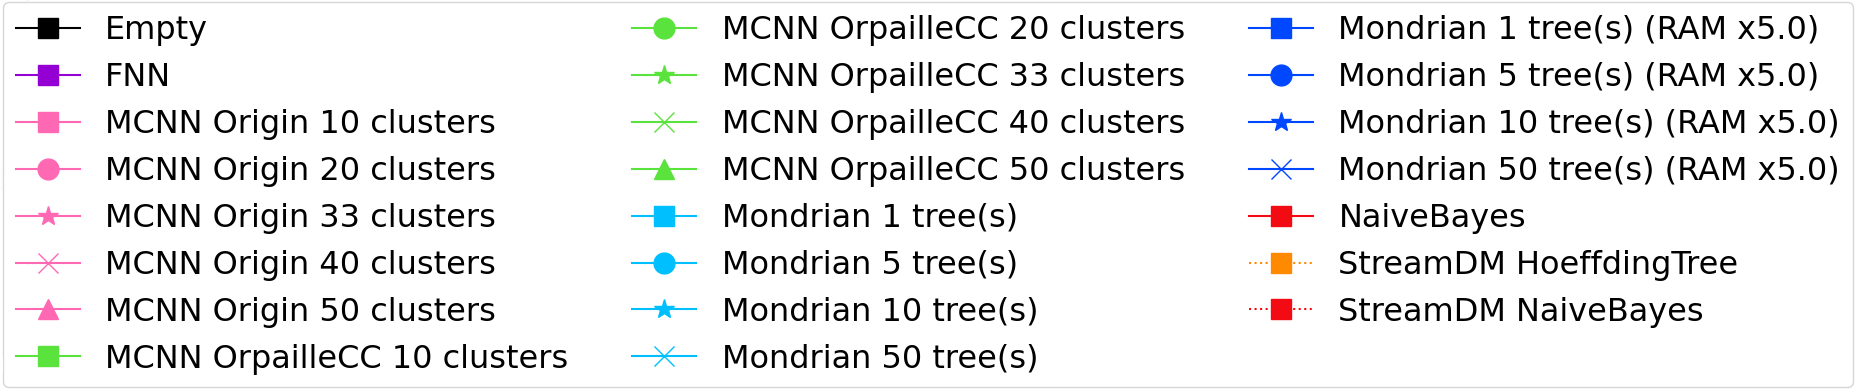
\includegraphics[width=0.8\linewidth]{figures/legend.png}
	\begin{subfigure}[t]{.49\linewidth}
		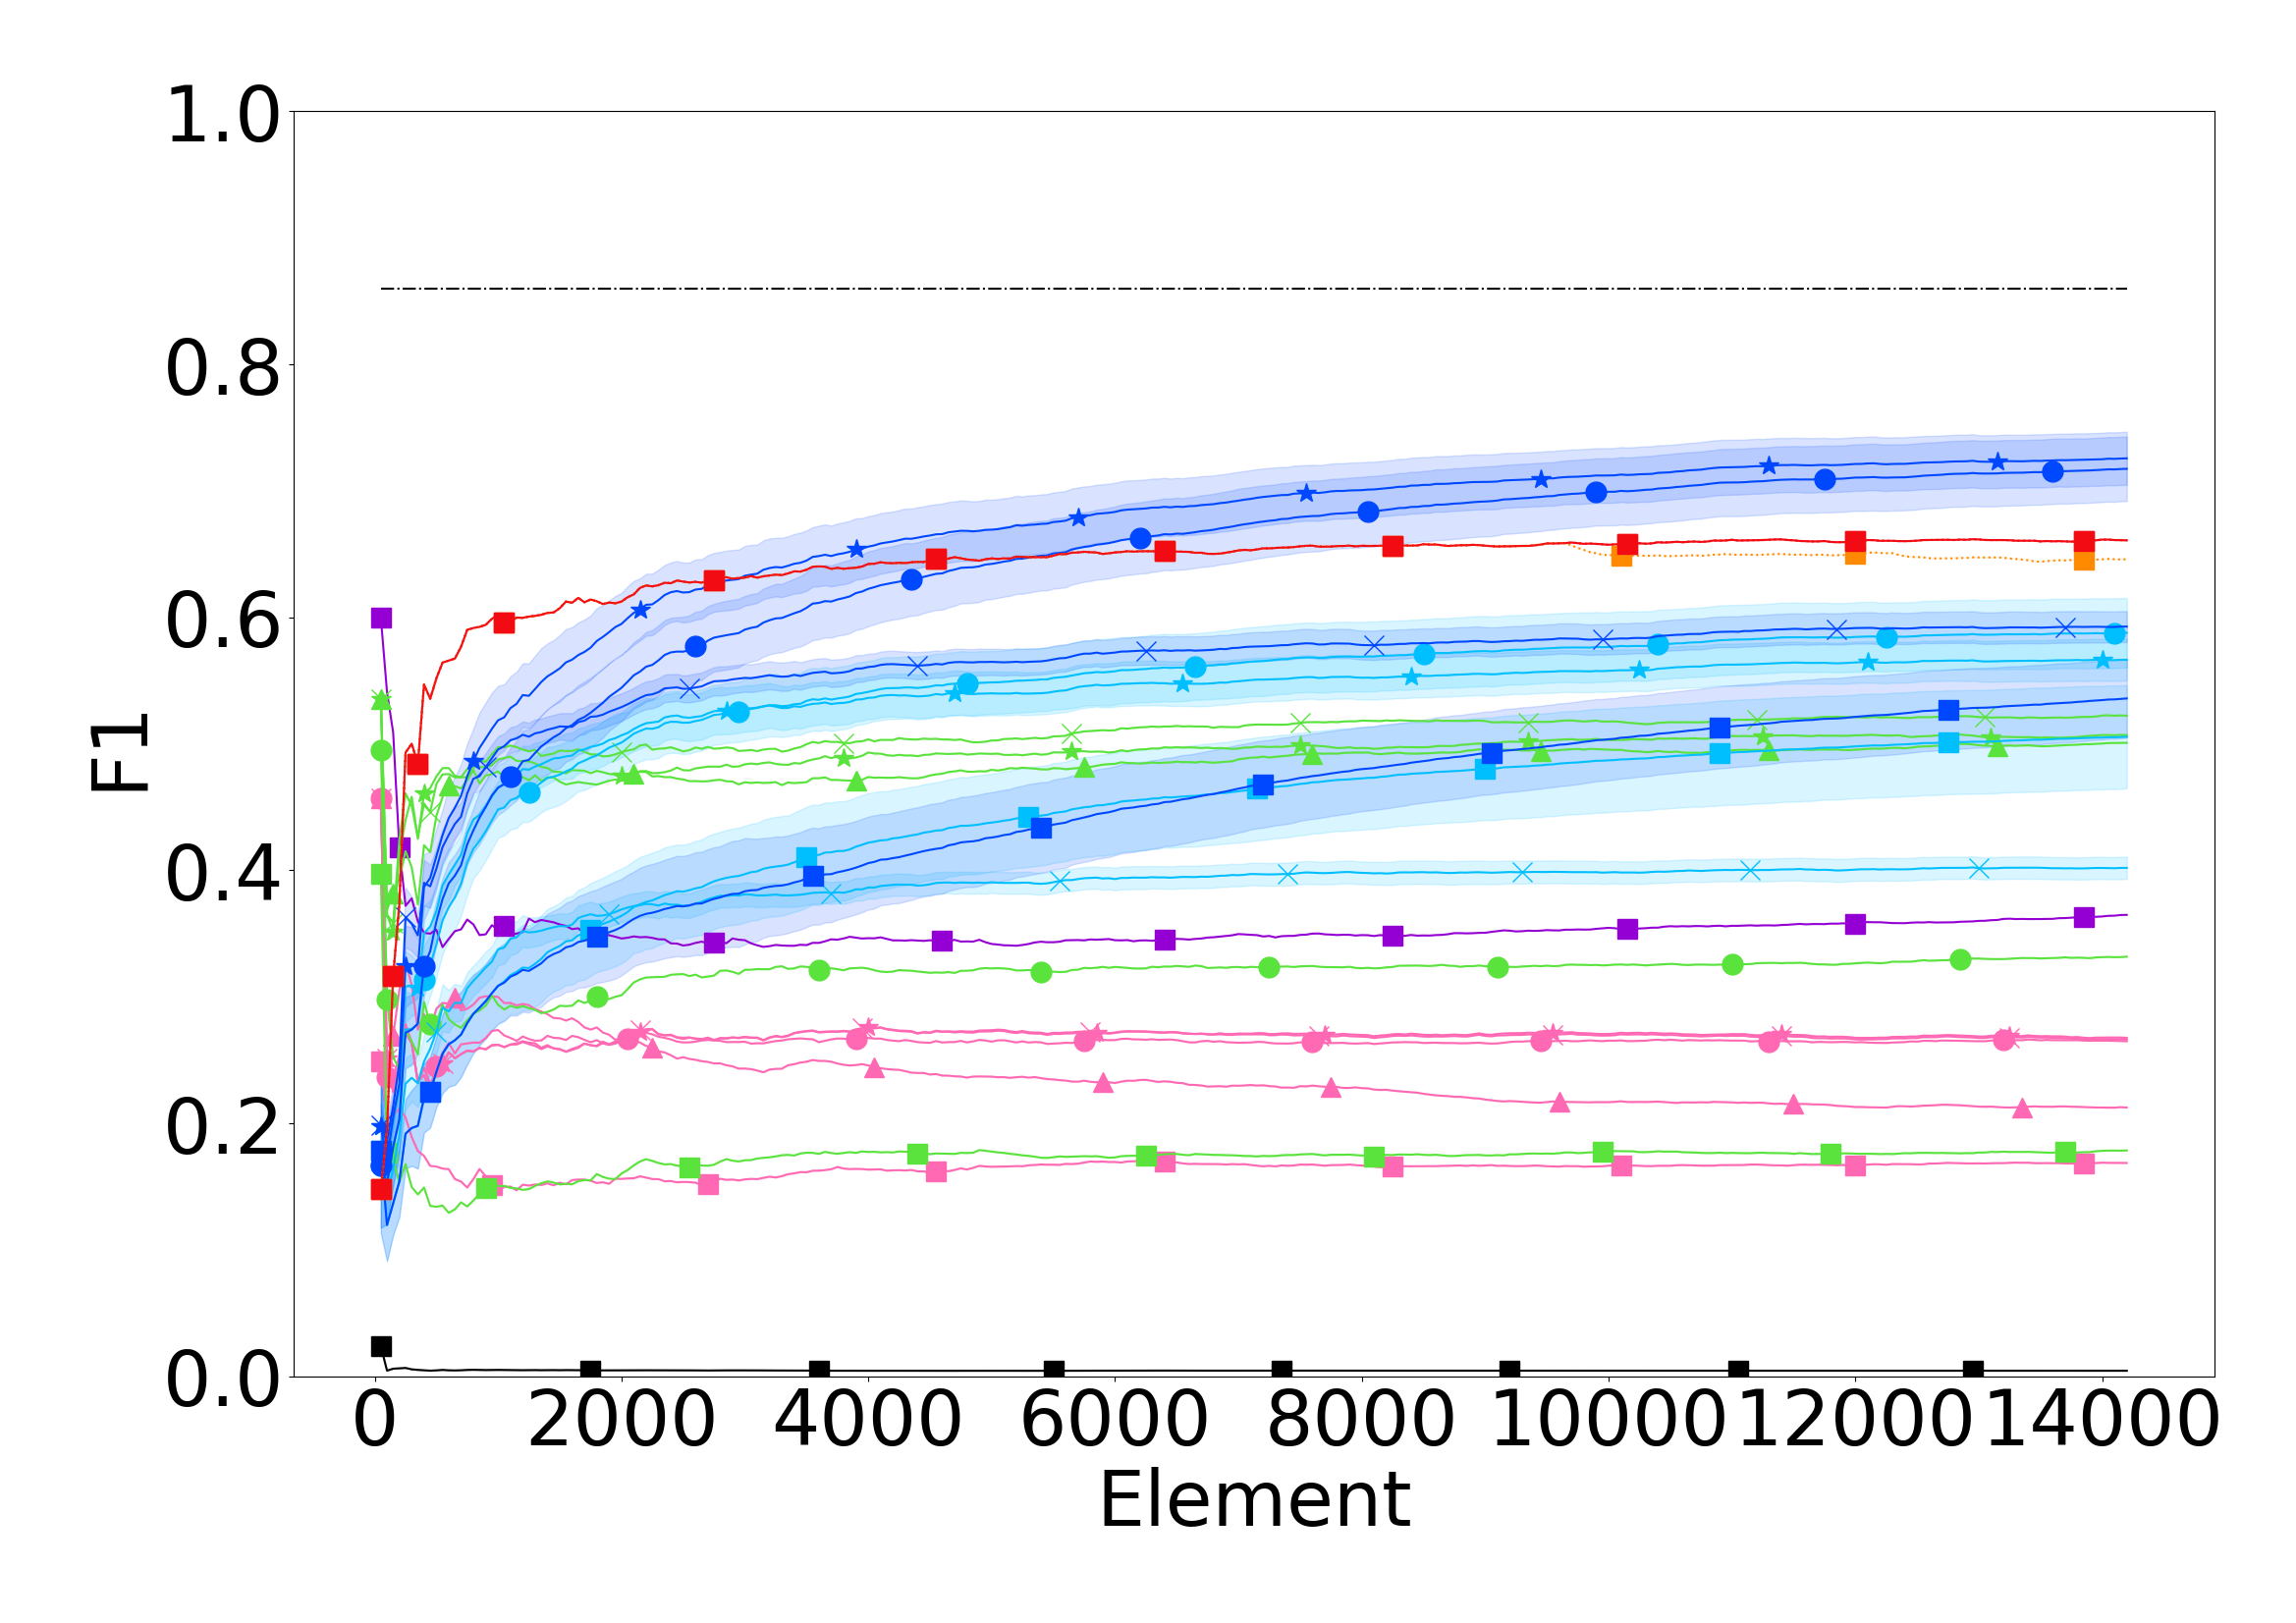
\includegraphics[width=\linewidth]{figures/results/banos_6_f1_std.png}
		\caption{\banosdataset}
		\label{fig:f1-banos}
	\end{subfigure}
	\begin{subfigure}[t]{.49\linewidth}
		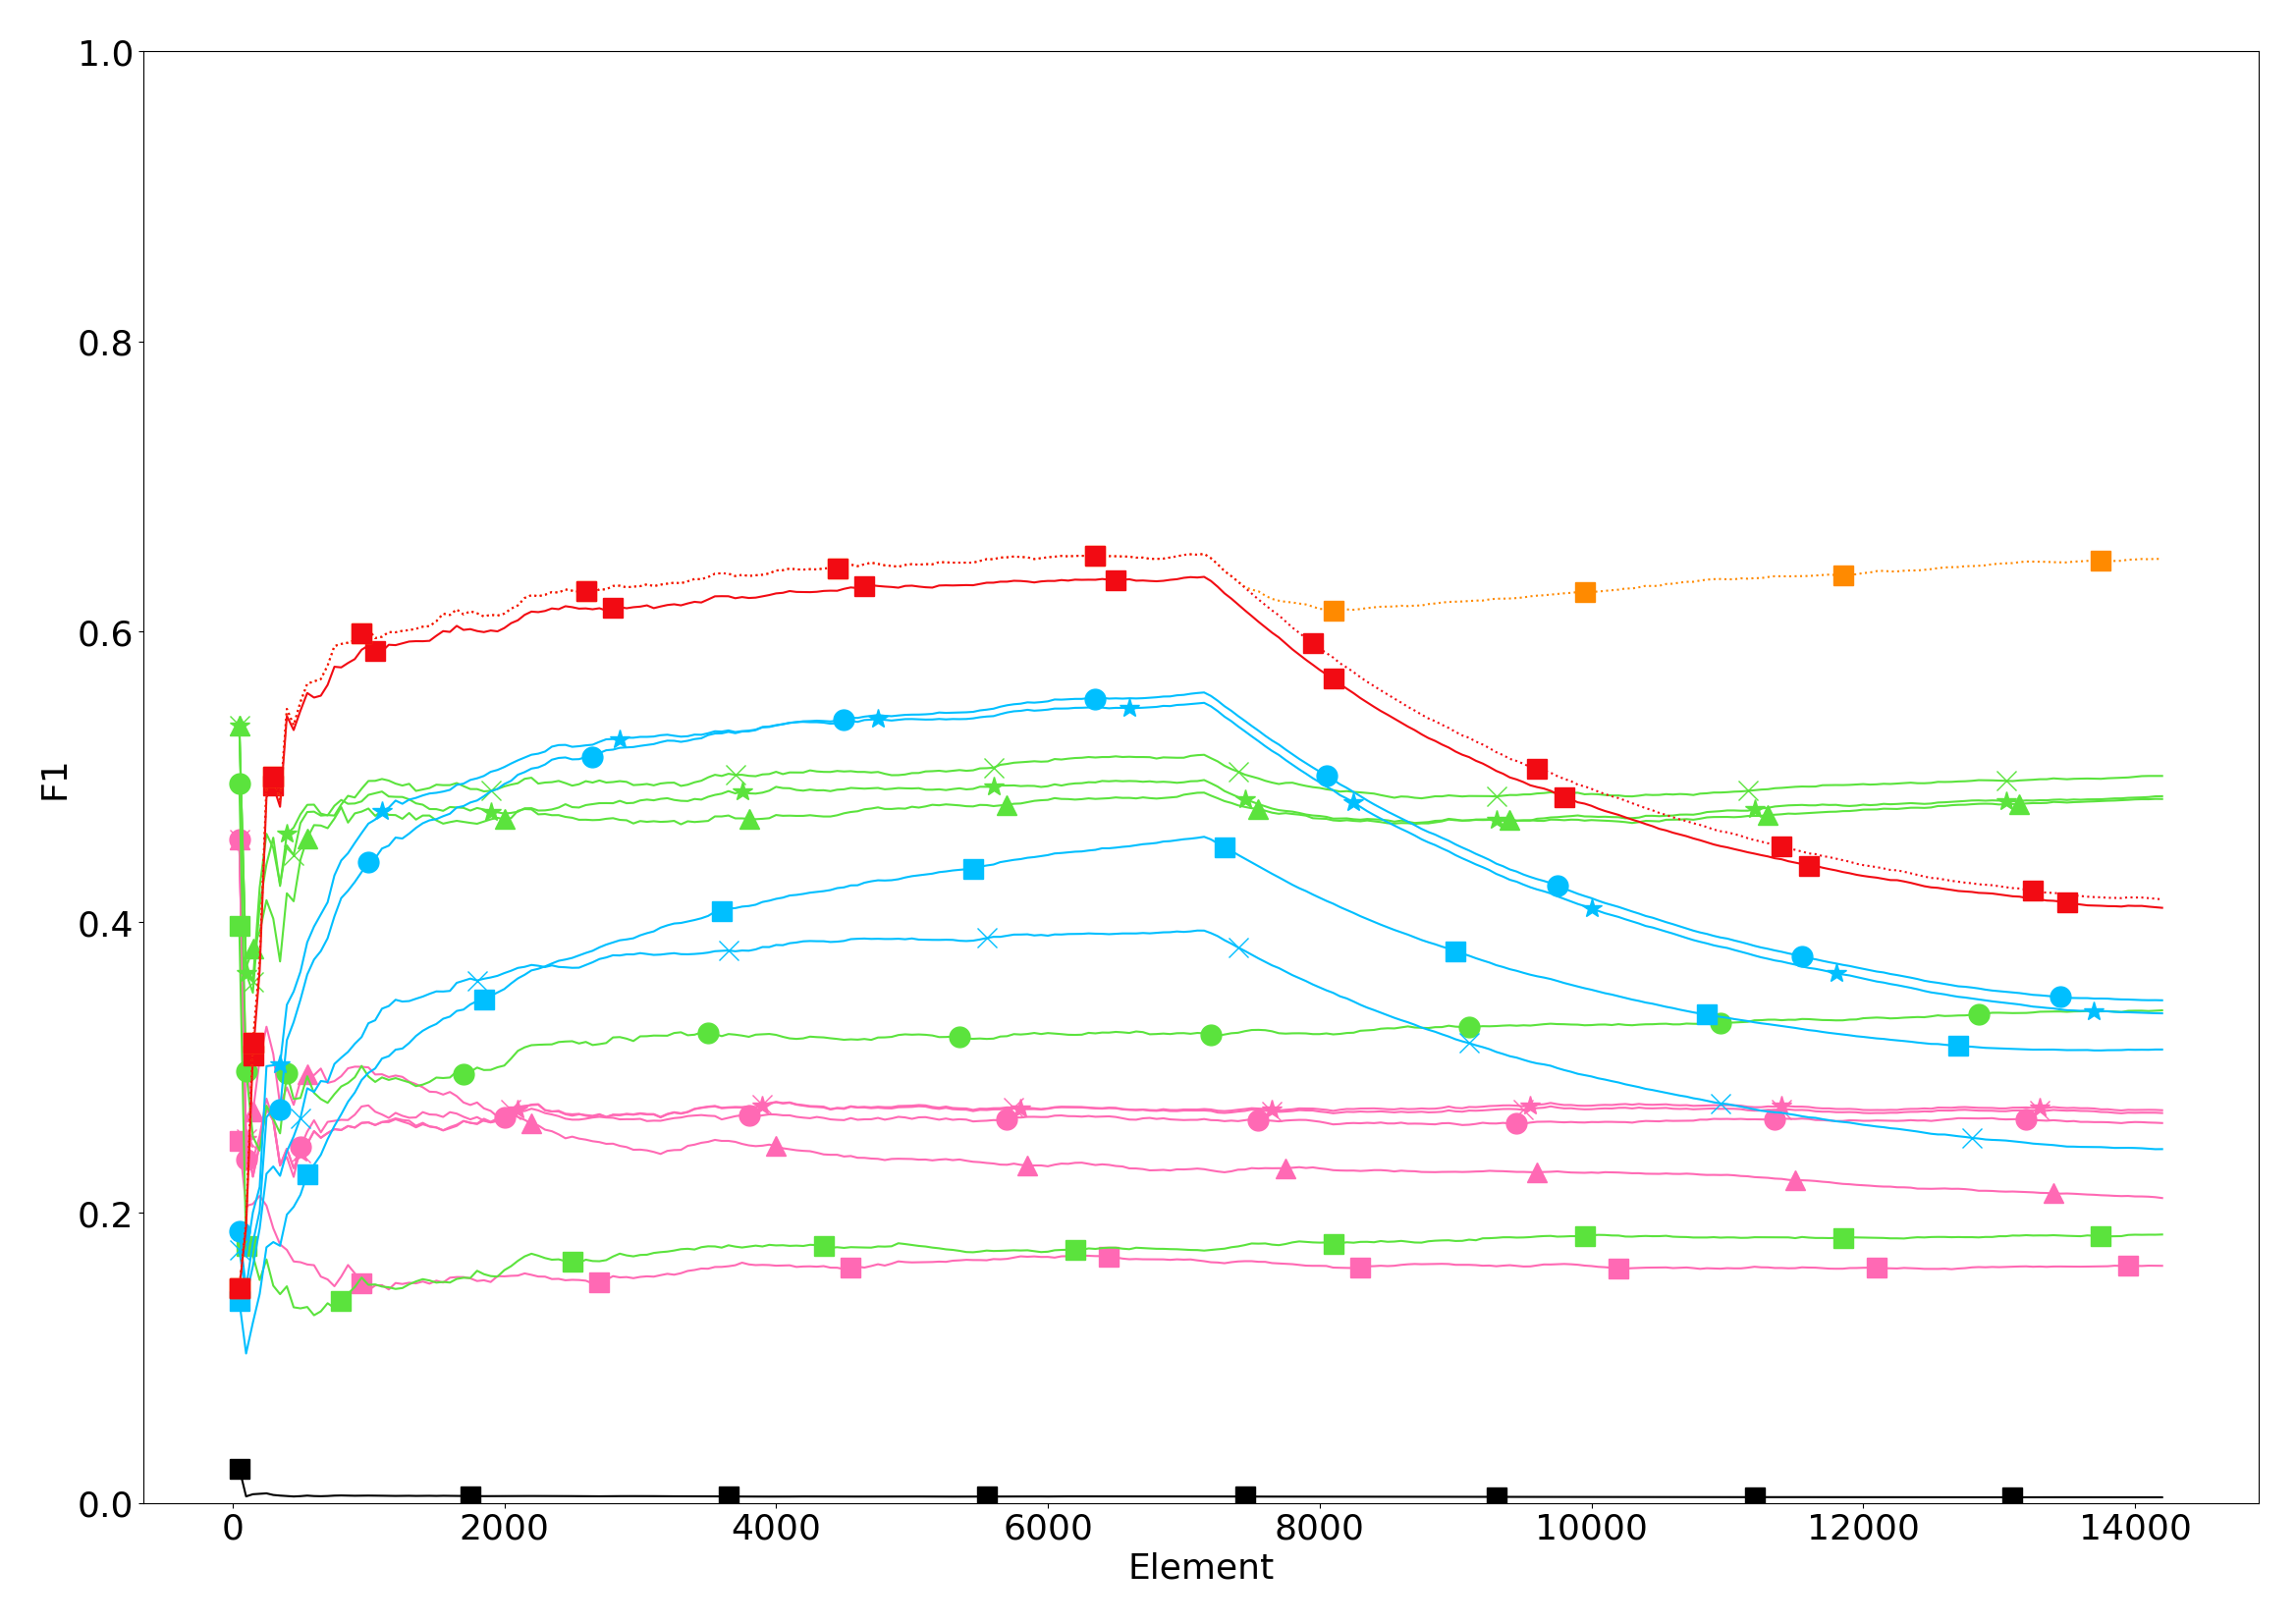
\includegraphics[width=\linewidth]{figures/results/drift_6_f1.png}
		\caption{\banosdataset (with Drift)}
		\label{fig:f1-drift}
	\end{subfigure}\\
	\begin{subfigure}[t]{.49\linewidth}
		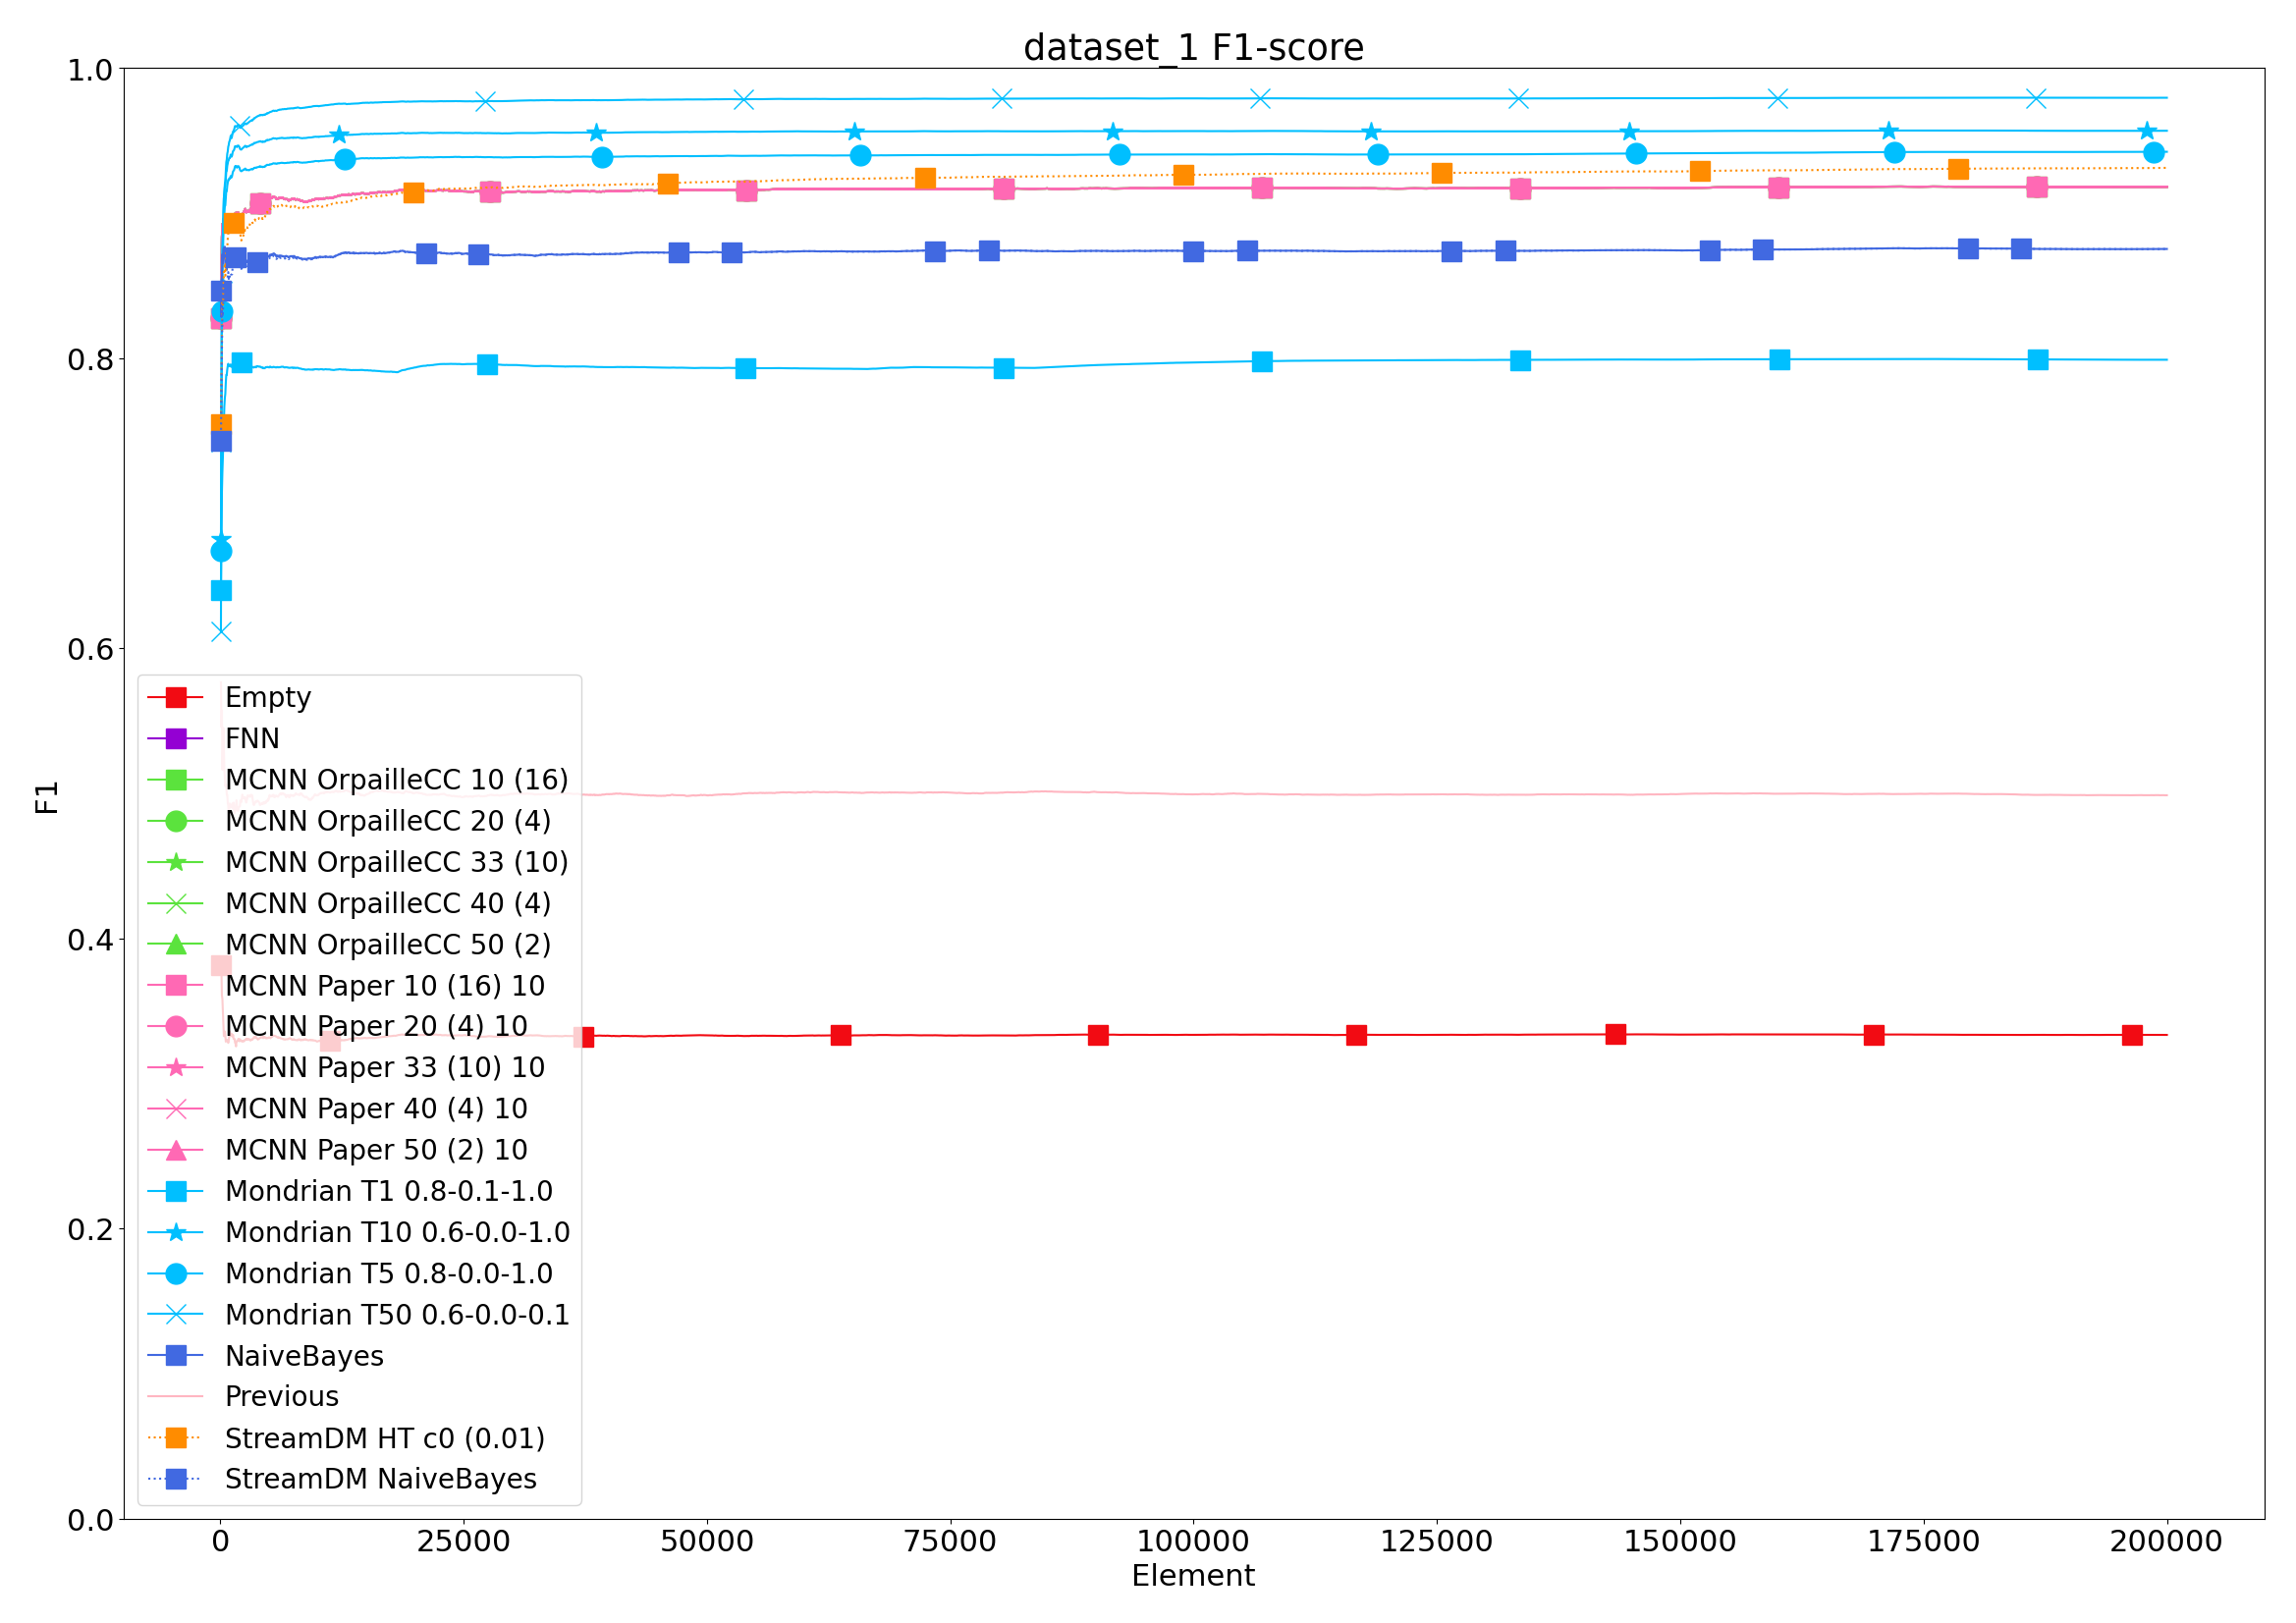
\includegraphics[width=\linewidth]{figures/results/dataset_1_f1.png}
		\caption{Hyperplane (MOA)}
		\label{fig:f1-dataset_1}
	\end{subfigure}
	\begin{subfigure}[t]{.49\linewidth}
		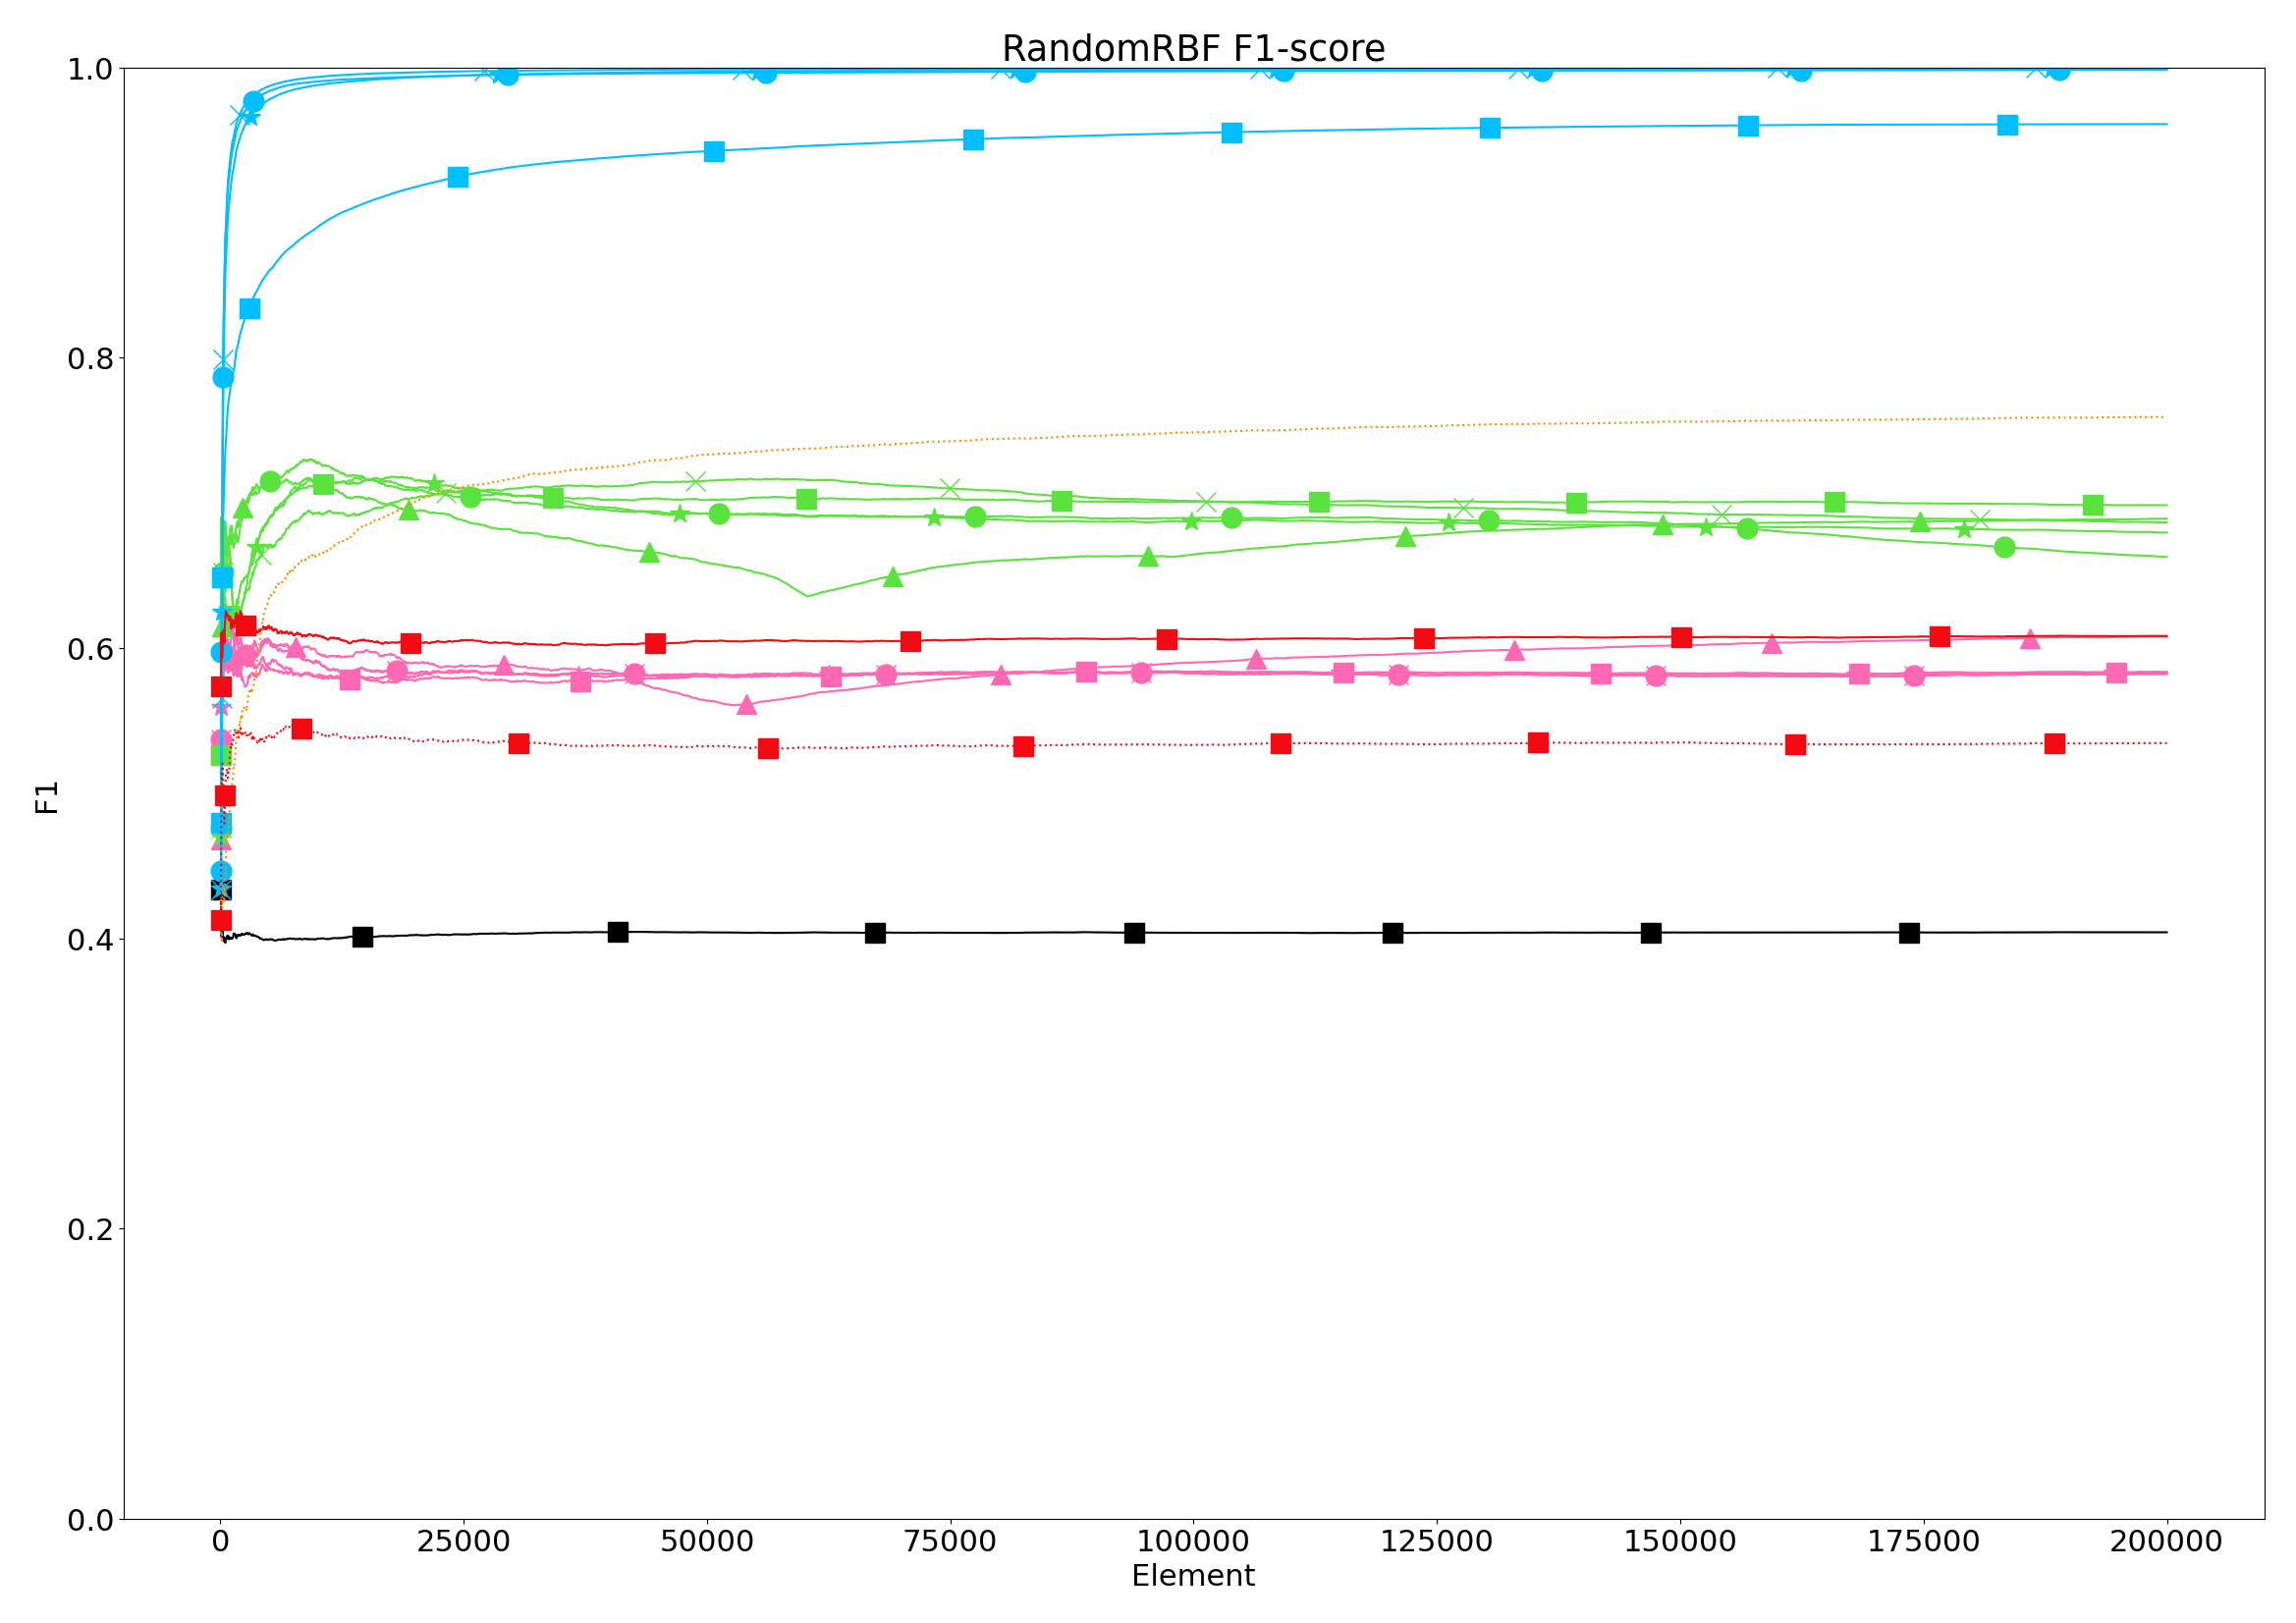
\includegraphics[width=\linewidth]{figures/results/dataset_2_f1.png}
		\caption{RandomRBF (MOA)}
		\label{fig:f1-dataset_2}
	\end{subfigure}\\
	\begin{subfigure}[t]{.49\linewidth}
		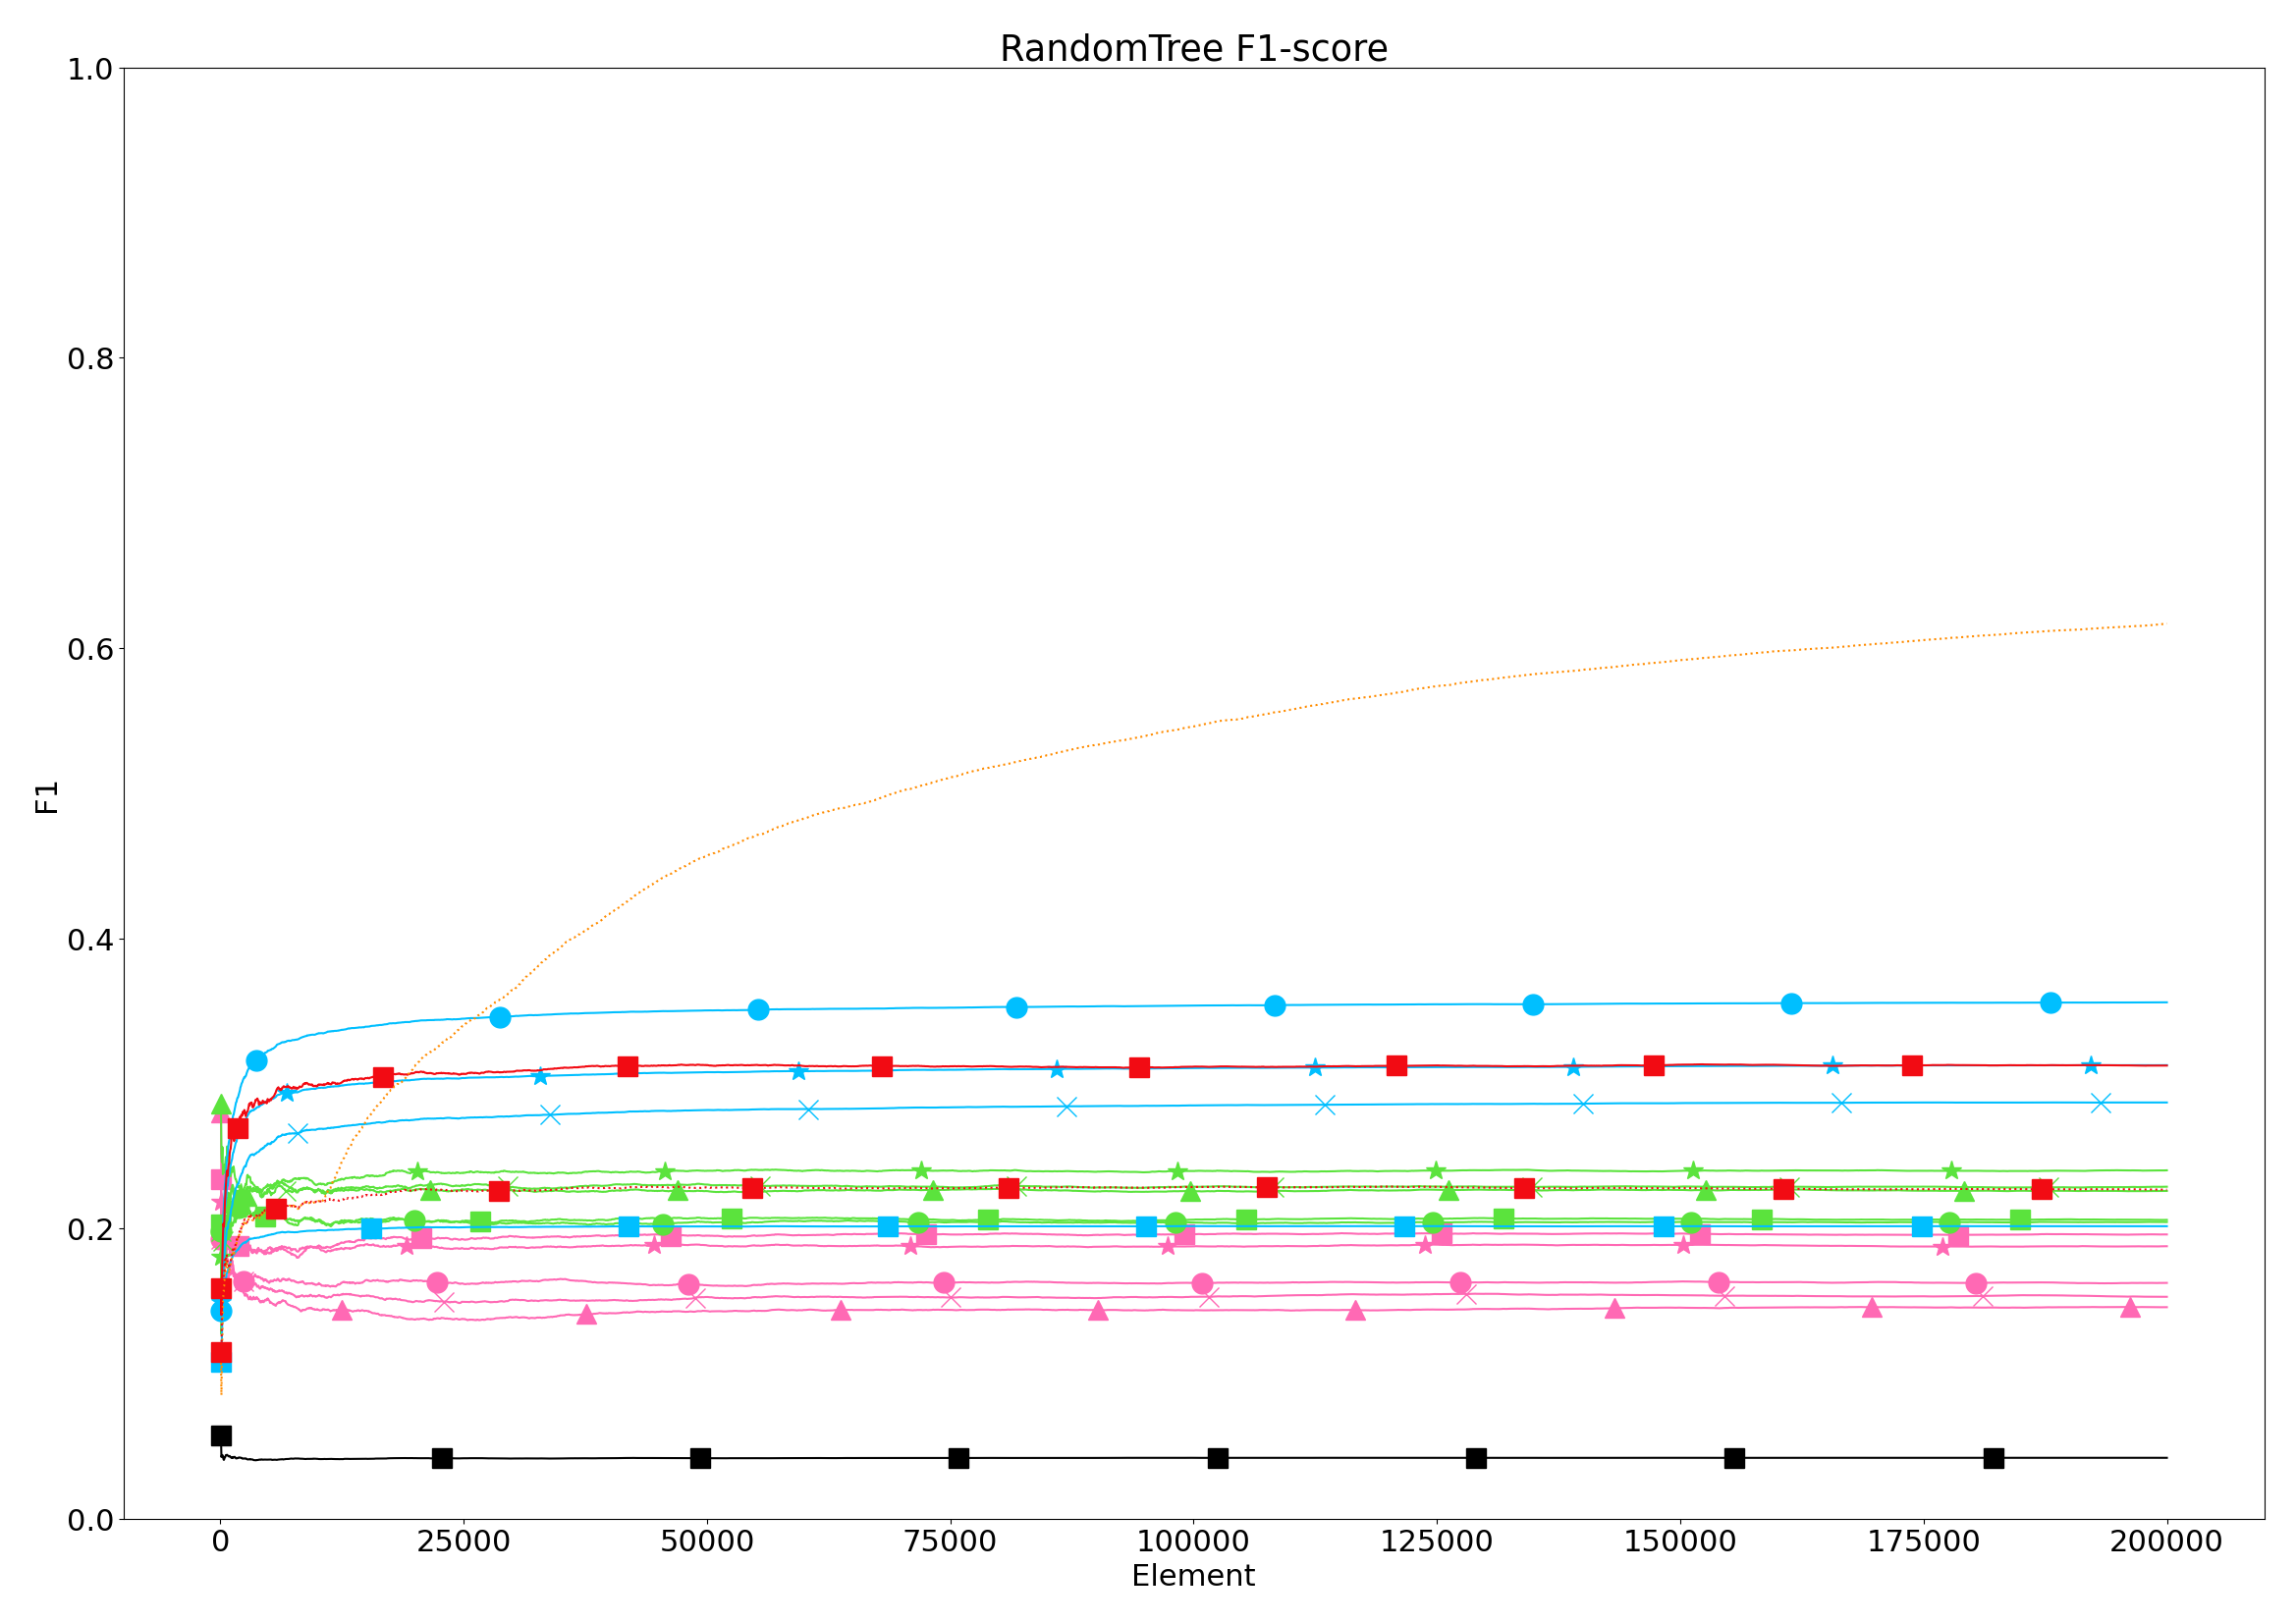
\includegraphics[width=\linewidth]{figures/results/dataset_3_f1.png}
		\caption{RandomTree (MOA)}
		\label{fig:f1-dataset_3}
	\end{subfigure}
	\begin{subfigure}[t]{.49\linewidth}
		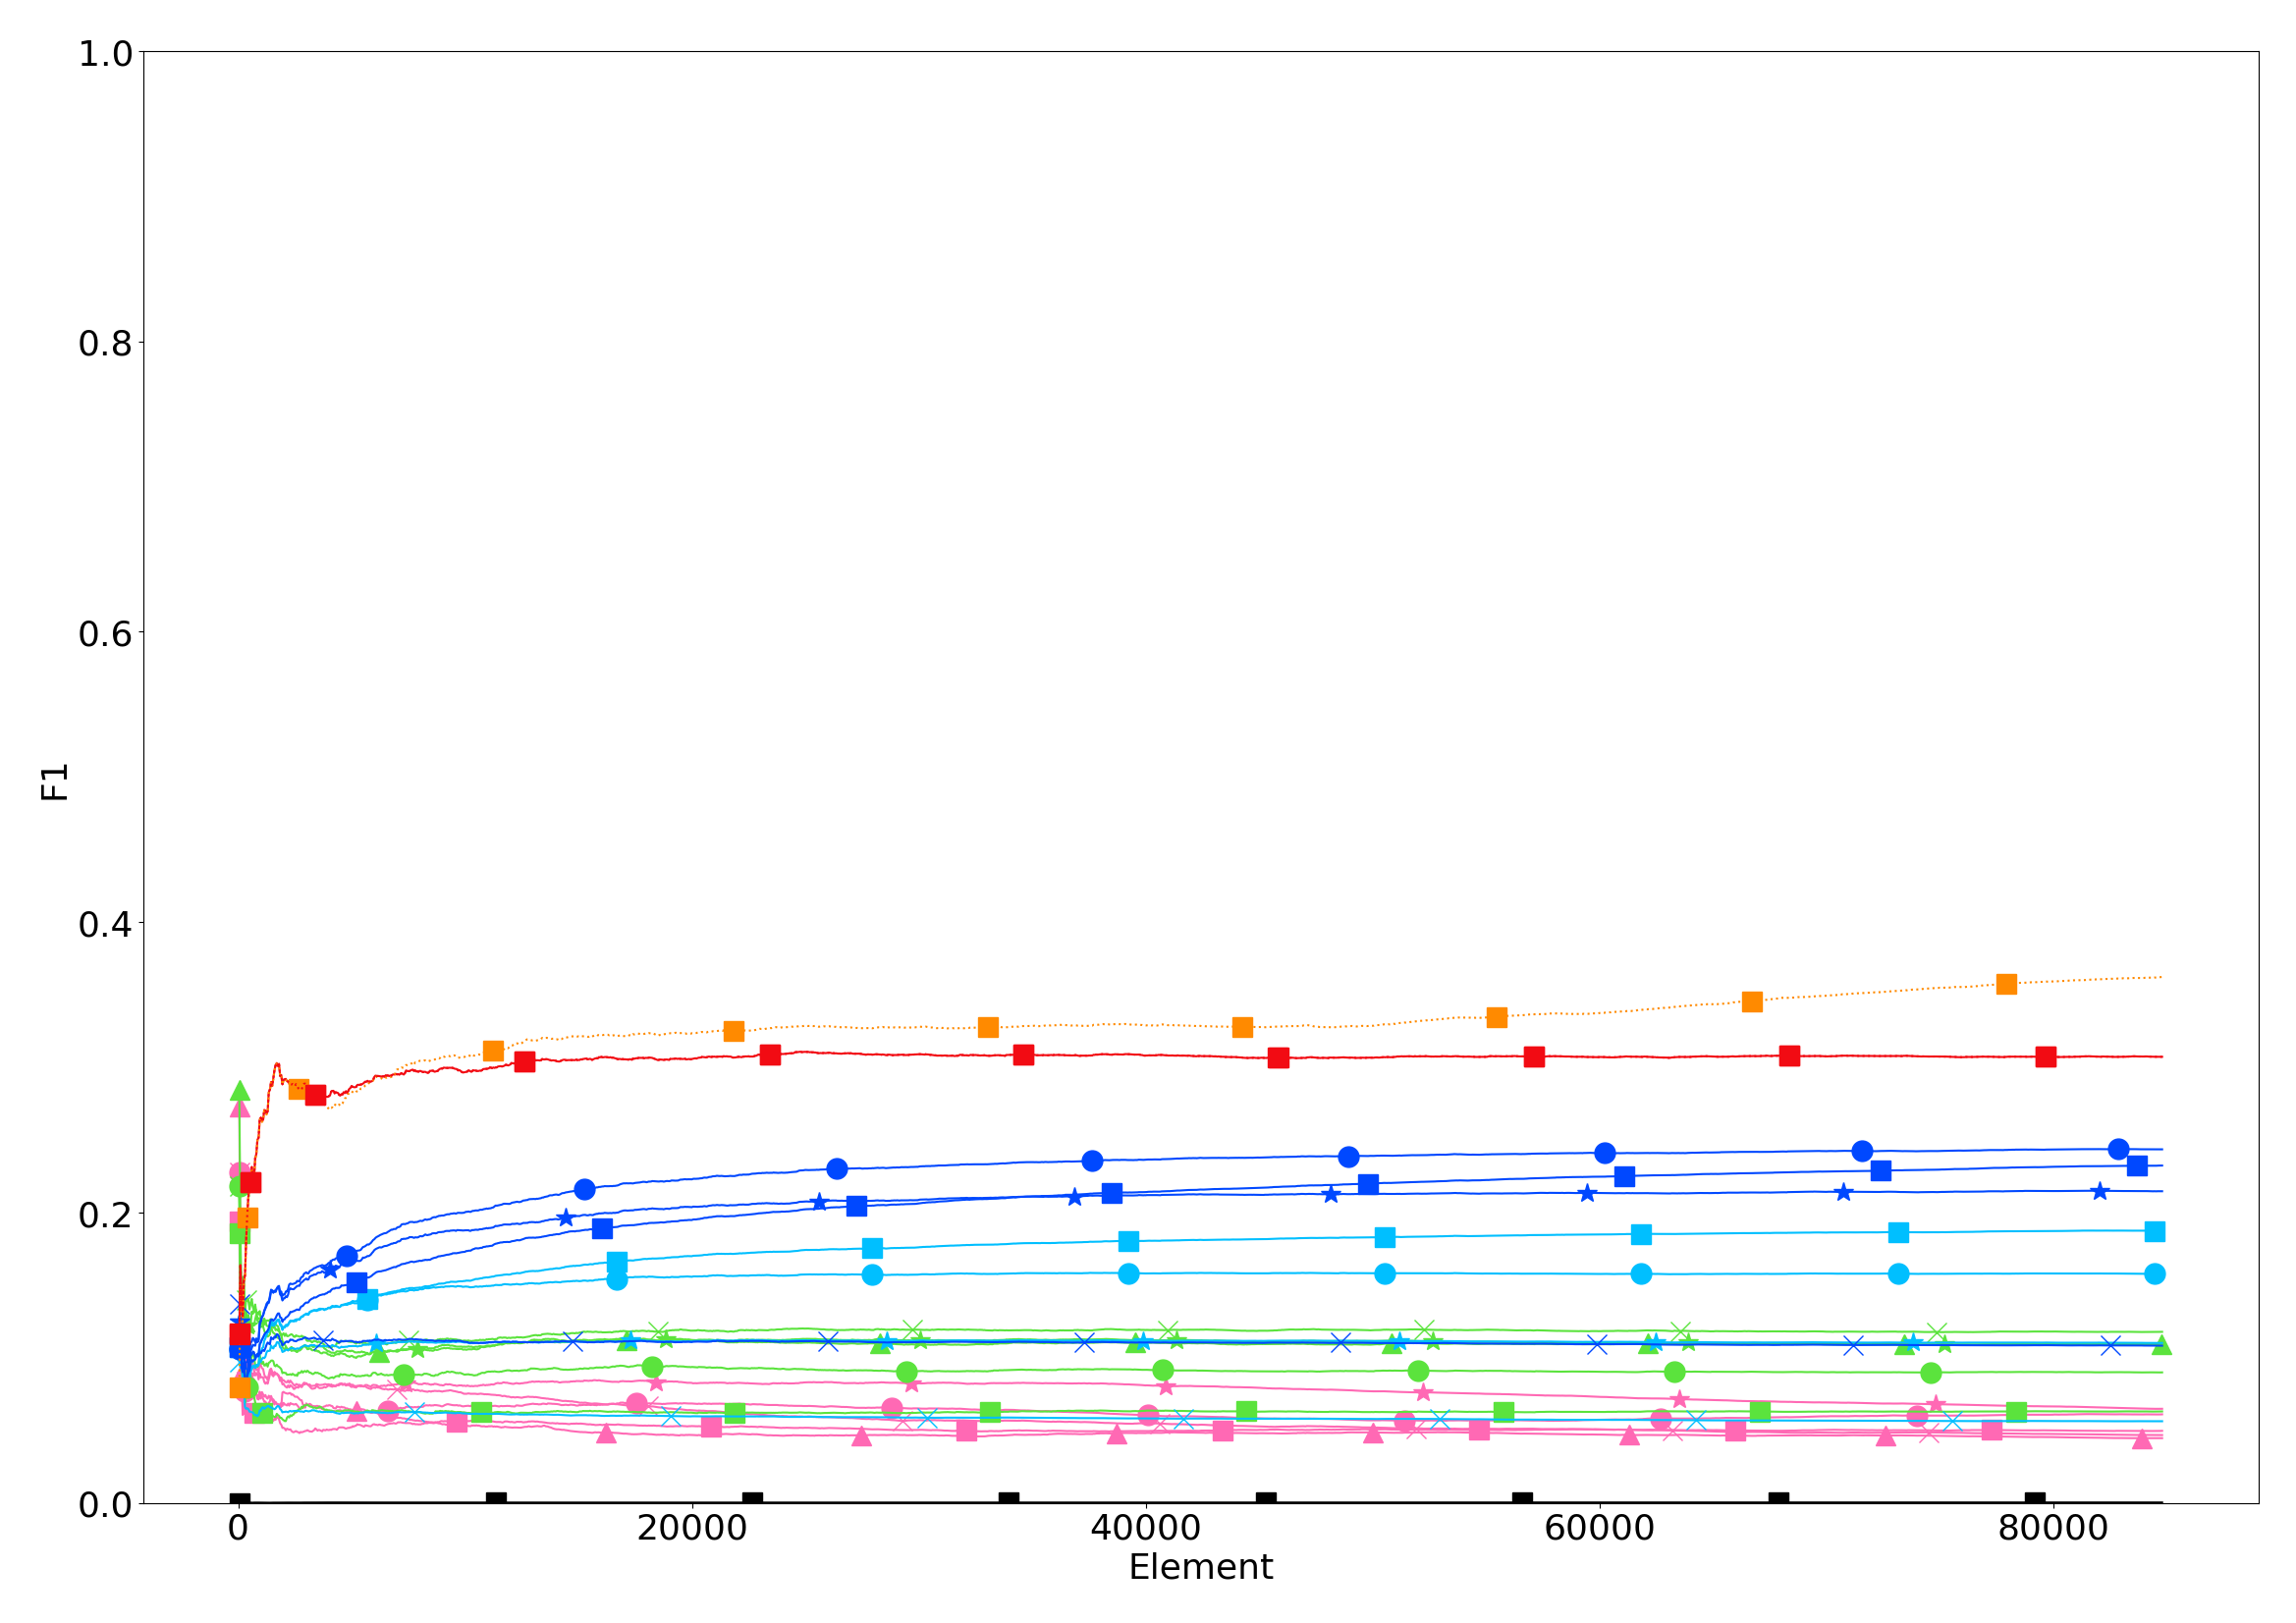
\includegraphics[width=\linewidth]{figures/results/recofit_6_f1.png}
		\caption{\recofitdataset}
		\label{fig:f1-recofit}
	\end{subfigure}
	\caption{F1 scores for the six datasets (average over 20 repetitions). The
		horizontal dashed black line indicate the offline \knn F1 score.}
	\label{fig:f1}
\end{figure*}

\section{Results}
This section presents our benchmark results and the corresponding
hyperparameter tunning experiments.

\subsection{F1 score}
Figure~\ref{fig:f1} compares the F1 scores obtained by all classifiers on the
six datasets.

%General description
F1 scores vary greatly across the datasets. While the highest
observed F1 score is above 0.95 on the Hyperplane and RandomRBF datasets,
it barely reaches 0.65 for the \banosdataset dataset, and it remains under
0.4 on the \recofitdataset and RandomTree datasets. This trend is
consistent for all classifiers.

%Offline observations
The offline \knn used as comparison achieves better F1 scores than all other
classifiers except for the \mondrianforest on the Hyperplane and the RandomRBF.
In particular, these F1 scores are lower than what is observed in the literature.
Indeed, on \banosdataset \knn only reach 0.86 when \cite{behzad2019} achieves
0.92 and \cite{Banos_2014} reaches 0.96. Similarly, \cite{behzad2019} reaches
0.65 on \recofitdataset dataset when we only achieve 0.4.

%Hoeffding and Naïve Bayes description when they are the best
The \naivebayes and the \hoeffdingtree stand out on the two real datasets
(\banosdataset and \recofitdataset) even though the F1 scores observed remained
low (0.6 and 0.35) compared to offline \knn (0.86 and 0.40). Additionally, the
\hoeffdingtree achieves outstanding performances on the RandomTree dataset and
\banosdataset dataset with a drift.

%Explanation of their F1 score similarity
Except for the \banosdataset dataset, the \hoeffdingtree F1 score is better than
the \naivebayes. Both F1 scores start close because the \hoeffdingtree uses a
\naivebayes in its leaves.  However, they start diverging most likely because
the \hoeffdingtree improves by reshaping its tree structure.  This is caused by
a sufficient amount of element and the difference is more noticeable when a
concept drift occurs.

%Mondrian when at best
On two synthetic datasets, Hyperplane and RandomRBF, the \mondrianforest (cyan)
with 10 trees achieves the best performances($> 0.95$), above the offline \knn.
Additionally, the \mondrianforest with 5 or 10 trees ranks third on the two real
datasets.

%Mondrian discussion
Surprisingly, a \mondrianforest (cyan) with 50 trees performs worse than 5 or 10
trees on most datasets. The only exception is the Hyperplane dataset where
50 trees F1 score is between 5 and 10 trees. This is due to the fact that
our \mondrianforest implementation is memory bounded, which is
useful on connected objects but limits tree growth when the allocated memory is
full. Because 50 trees fill the memory faster than 10 or 5 trees, the
classifier learning is blocked faster, when the trees have not learned enough
from the data.

%Bounded memory discussion
We differentiate bounded memory from constant space complexity because in the
first case, a limited amount of memory may force the classifier to find a way
around this lack of memory: stop growing or making space for new data.
Therefore, influencing its performance.  On the other hand, a constant space
complexity is a feature of a classifier and its performances are not expected
to change no  matter the amount of memory available. The classifier is simply
supposed to fail without the required amount of memory. From the algorithm
involved in this study, \mondrianforest has a bounded memory policy while
\naivebayes is a classifier with a constant space complexity.

%Mondrian RAMx5
This dependency of the \mondrianforest to memory allocation is shown in
Figures~\ref{fig:f1-banos}-\ref{fig:f1-recofit}, where an additional
configuration with five-time more memory (total of 3MB) is shown (deep blue)
whereas the \mondrianforest (cyan) has 600~KB.  The memory increase induces an
F1 score difference greater than 0.1, except when only one tree is used. In
which case the improvement caused by the memory is less than 0.05. Note that the
selected memory-bound does not match all situations. Indeed, depending on
the connected object the memory limit can range from a few KB to GB.

%MCNN observations
The \mcnn OrpailleCC stands out in Figure~\ref{fig:f1-drift} where it ranks
second by adapting to a concept drift.  On other datasets, \mcnn OrpailleCC is
ranked after the \mondrianforest and the \hoeffdingtree, but above \mcnn
Original. This difference between the two \mcnns is presumably due to the fact
that \mcnn Origin removes clusters too fast even with a low participation
threshold.  On the real datasets (\banosdataset and \recofitdataset), we notice
that \mcnn OrpailleCC classifier appears to be learning faster than the
\mondrianforest, although \mondrianforest catches up after a few thousand
elements. Finally, we note that \mcnn stays quite lower than the offline \knn.

%FNN observation
Figure~\ref{fig:f1-banos} has shown that the \FNN has a low F1 score (0.36)
compared to other classifiers (above 0.5). It contradicts the results depicted
in~\cite{omid_2019} where \FNN achieves more than 95\% accuracy. The main
difference between~\cite{omid_2019} and this study comes from the training set.
In~\cite{omid_2019}, not only the training set includes examples from every
subjects, but also the windows are overlapping and wider than the ones we used.
Therefore, we expect the \FNN to have already encountered most of the datapoints
from the testing set. When instead of using only the first subject of the
\banosdataset dataset we used a sample of 10\% of of all datapoints in the
\banosdataset dataset, we managed to reach an F1 score slightly above 0.6, which
is close to the \naivebayes.

%FNN discussion
Note that the pre-training of the \FNN is slightly different from the other
classifiers. Indeed, the hyperparameters tuning of the other classifiers implies
that they start the testing phase with no prior knowledge of the dataset even
about the element seen in the tuning phase. On the other hand, the \FNN starts
with its weights already set, therefore we can say that it has already seen part
of the dataset. We proceed that way because it takes many epochs for the weights
to adjust correctly so if the weights were randomly initialized for the testing
phase, the \FNN would answer randomly.  We deviated from the method for the \FNN
classifier because neural networks have shown a wide range of classification
abilities depending on how they are used.  Therefore, we
followed~\cite{omid_2019} which exhibits high classification performance. Since
the \FNN model is tightly coupled with network structure and since we only
trained the model with subject 1 from \banosdataset, we only run \FNN on the
\banosdataset datasets.

%Variance
Figure~\ref{fig:f1-banos} includes the F1 score variance. Only the
\mondrianforest shows variability because it is the only classifier involving
randomness. The variance decreases with the number of trees, as expected.

%Concept drift
The \hoeffdingtree appears to be the most robust to concept drifts
(Figure~\ref{fig:f1-drift}), while the \mondrianforest and \naivebayes
classifiers are the most impacted. \mcnn classifiers are marginally impacted.
The low resilience of \mondrianforest to concept drifts can be attributed to
two factors. First, existing nodes in trees of a \mondrianforest cannot be updated.
Second, when the memory limit is reached, \mondriantrees cannot grow
or reshape their structure anymore.

%Naive Bayes and Naive Bayes
Finally, we note that the StreamDM and OrpailleCC implementations of
\naivebayes are indistinguishable from each other, which confirms our
implementation in OrpailleCC.

%One sensor
In this study, we focused on using one sensor rather than all the sensors
available in the real datasets. In the case of more sensor used, we would expect
an F1 score improvement for all classifiers because they would have access to
more data in order to discriminate the classes. On the other hand, we would
expect an increase in the memory footprint because more sensors mean more
attribute extracted. This should have minimal impact on classifiers such as
\naivebayes because their footprint is already low. However, the
\mondrianforest, the \hoeffdingtree, and \mcnn memory footprints are expected to
grow significatively because more sensors means more attributes for each leaf or
cluster. In particular, we expect the \mondrianforest F1 score to be mitigated
by the decrease of memory induced by the increased leave size.

\begin{figure*}
	\begin{subfigure}[t]{.49\linewidth}
		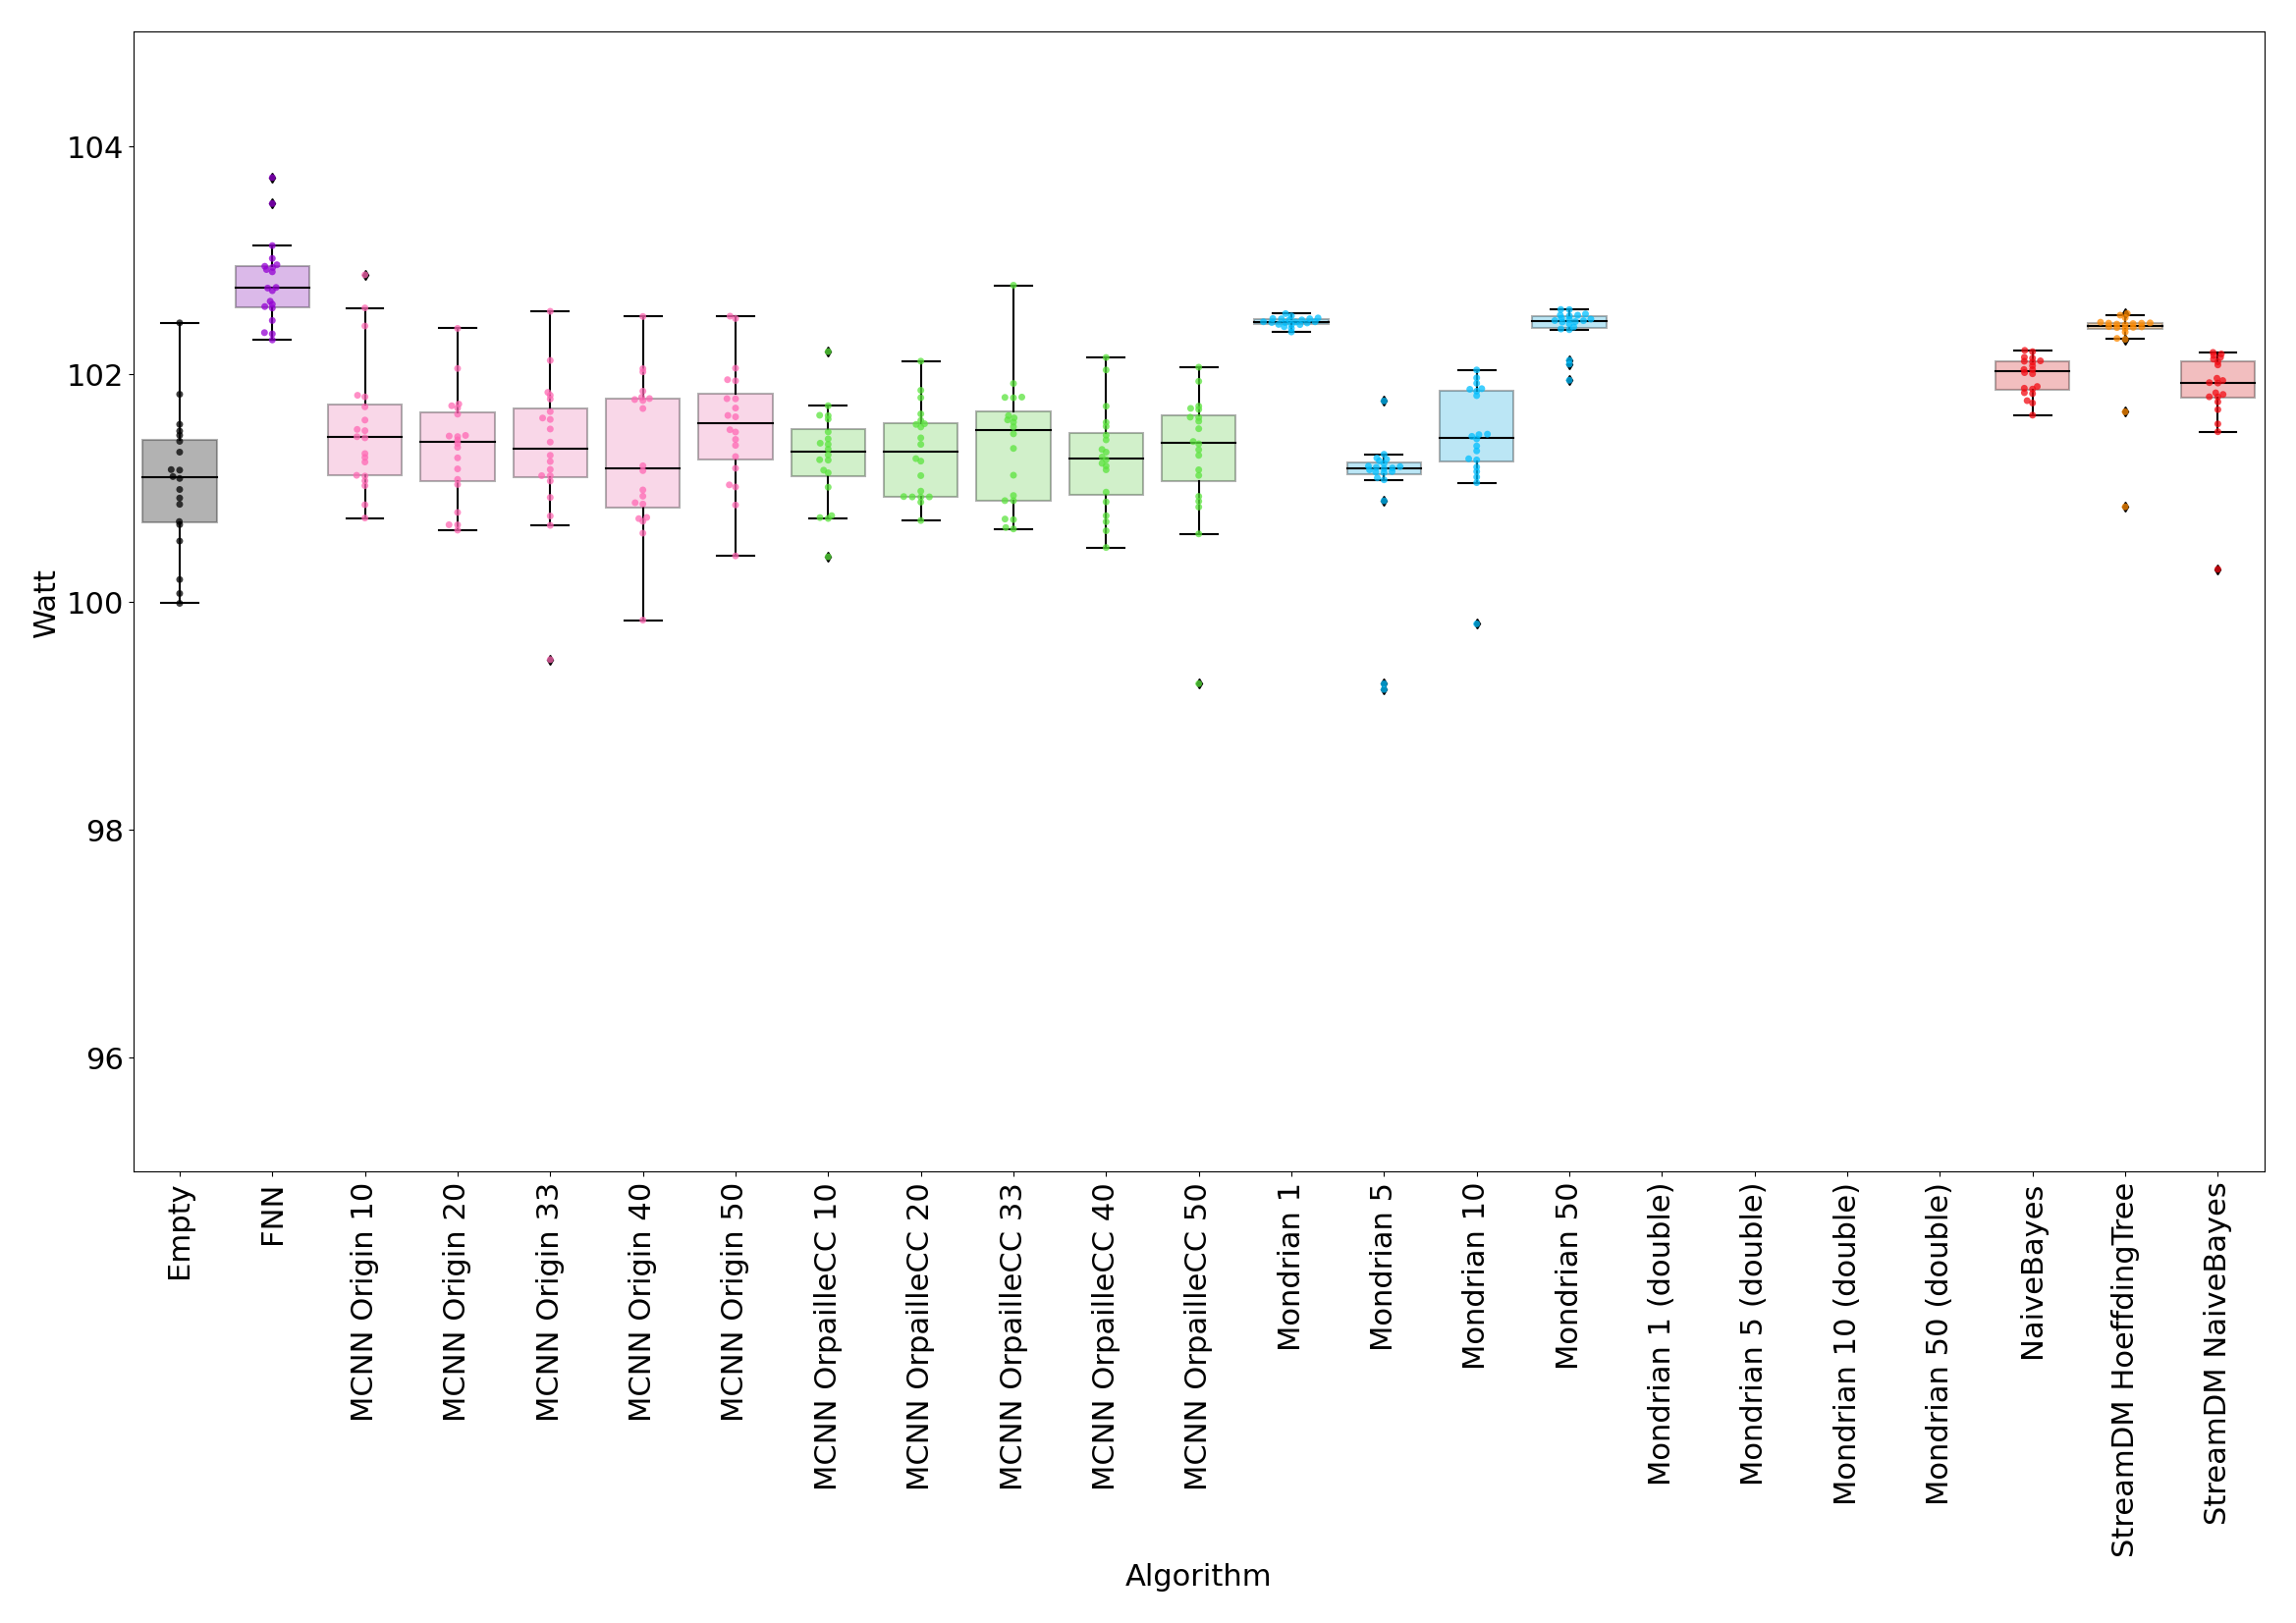
\includegraphics[width=\linewidth]{figures/results/banos_3_watt.png}
		\caption{\banosdataset}
		\label{fig:power-banos}
	\end{subfigure}
	\hfill
	\begin{subfigure}[t]{.49\linewidth}
		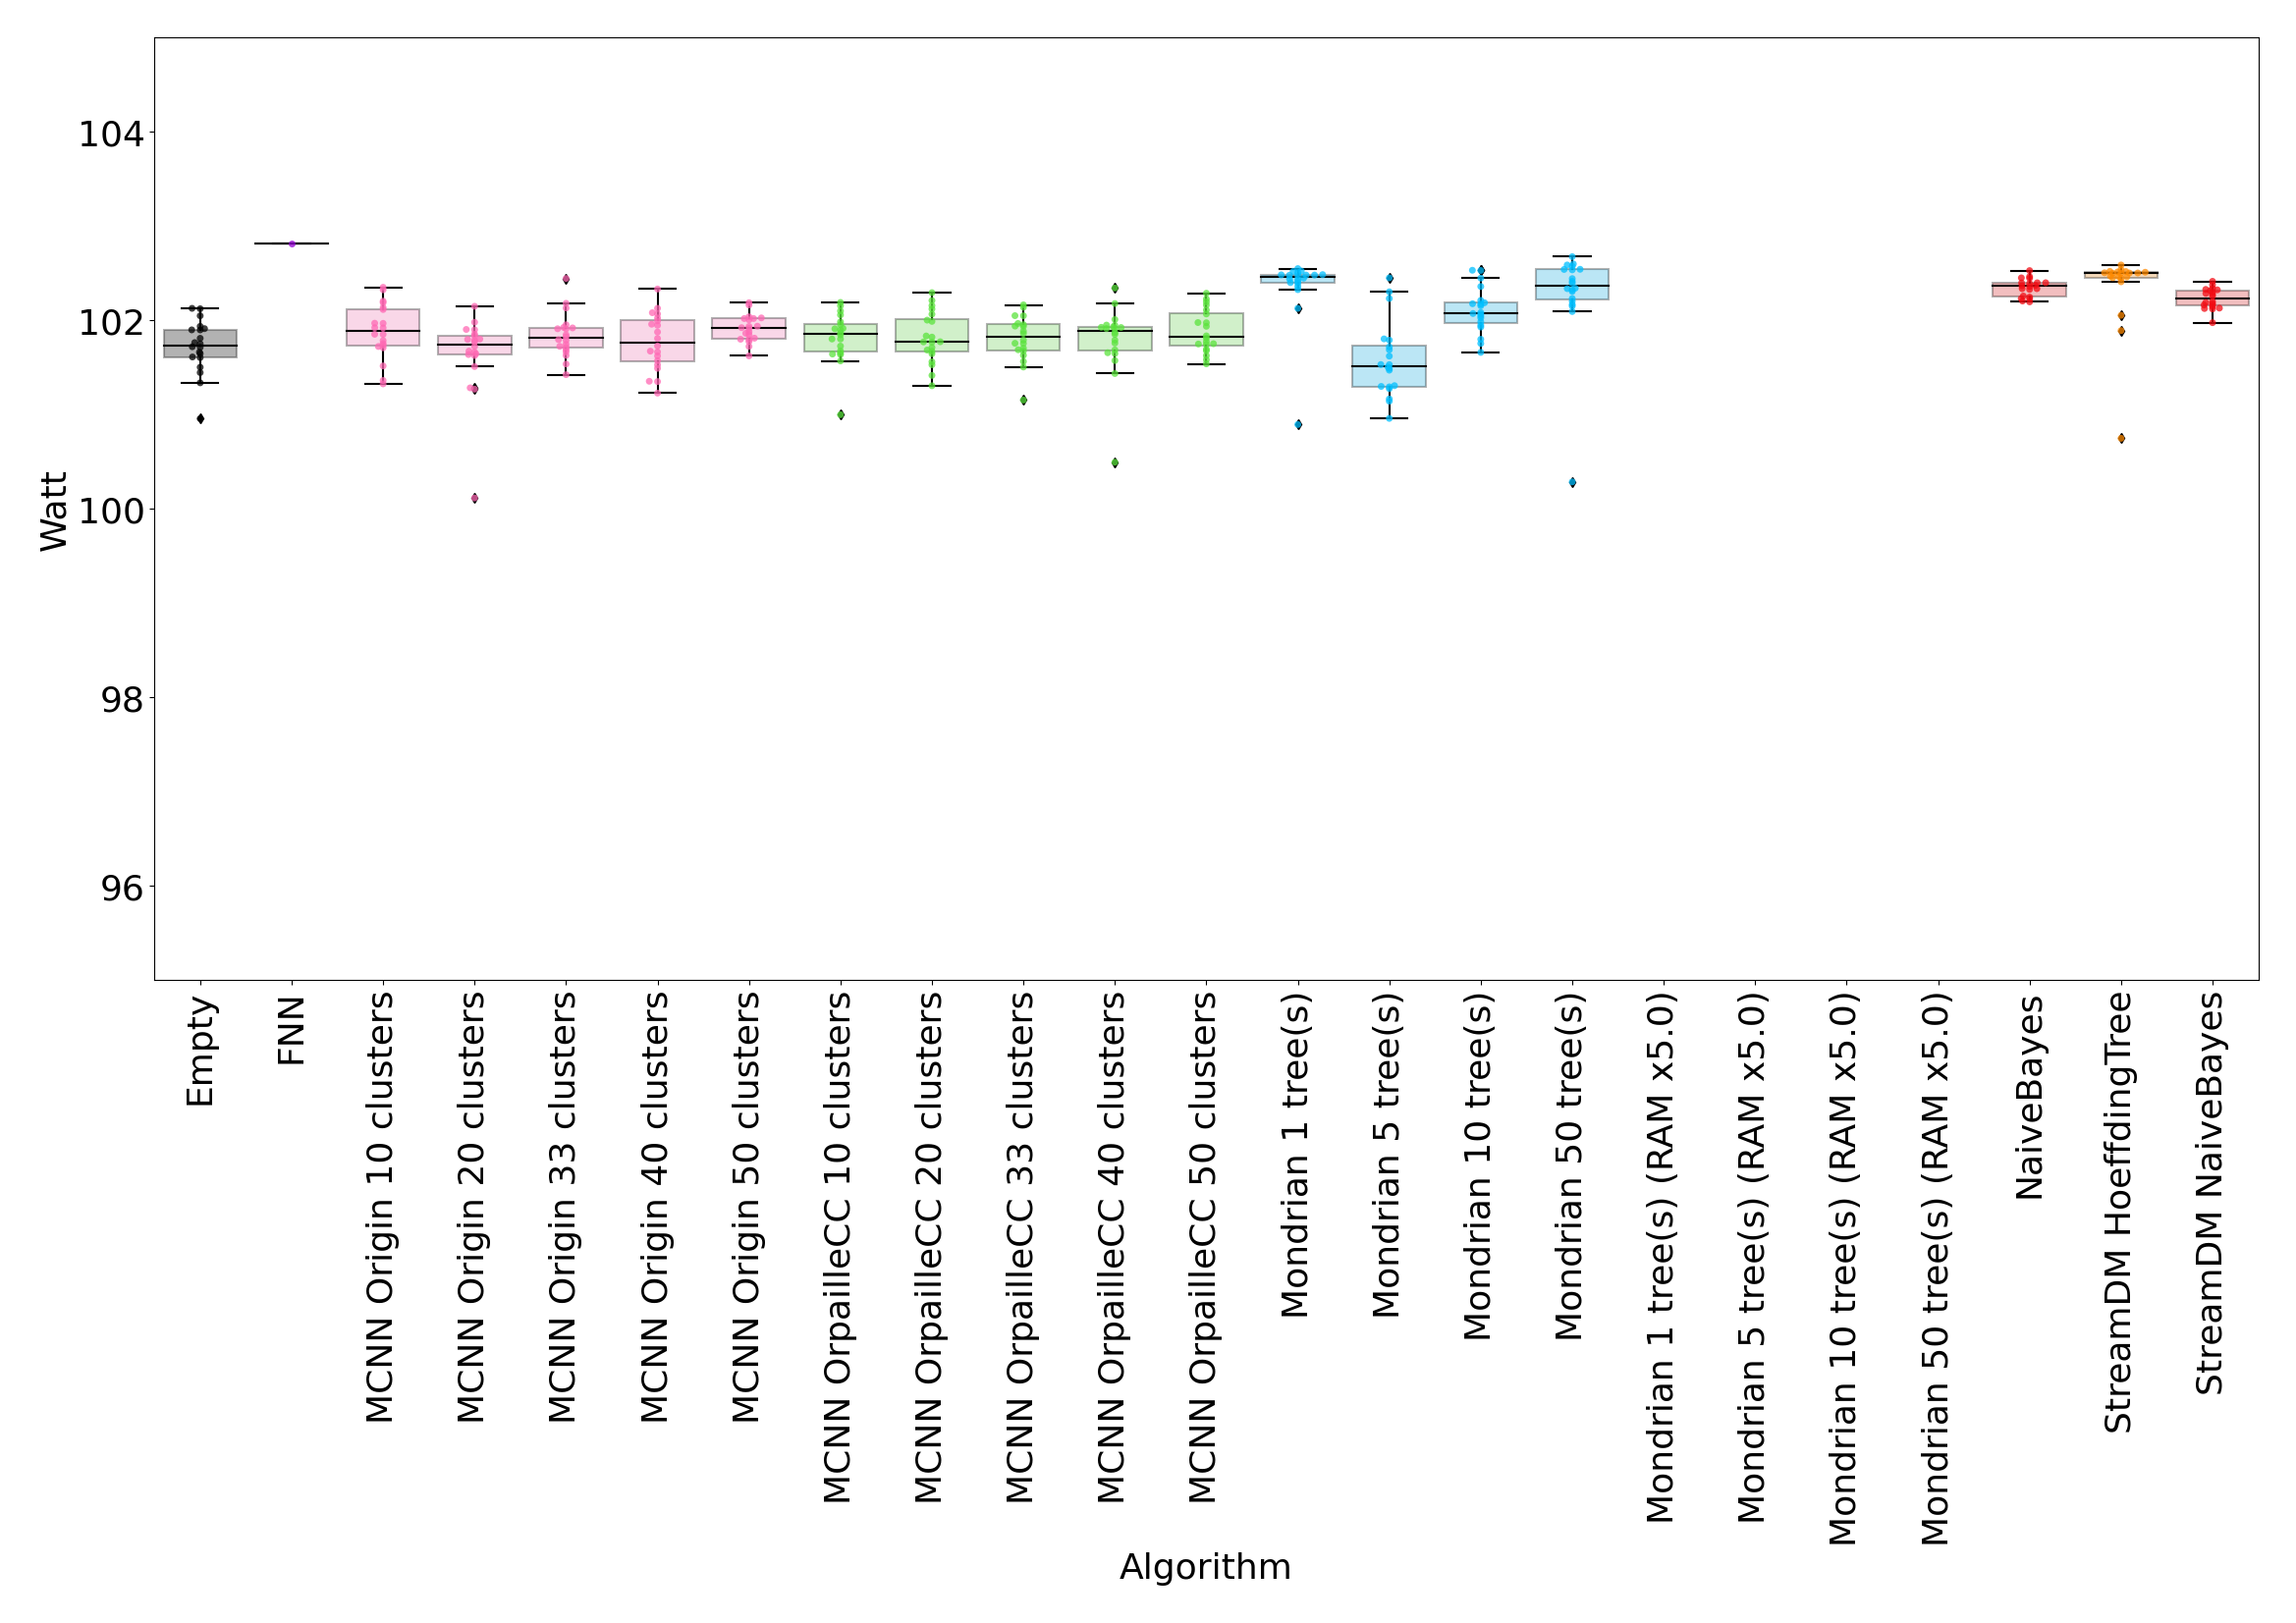
\includegraphics[width=\linewidth]{figures/results/drift_6_watt.png}
		\caption{\banosdataset with drift.}
		\label{fig:power-drift}
	\end{subfigure}\\
	\begin{subfigure}[t]{.49\linewidth}
		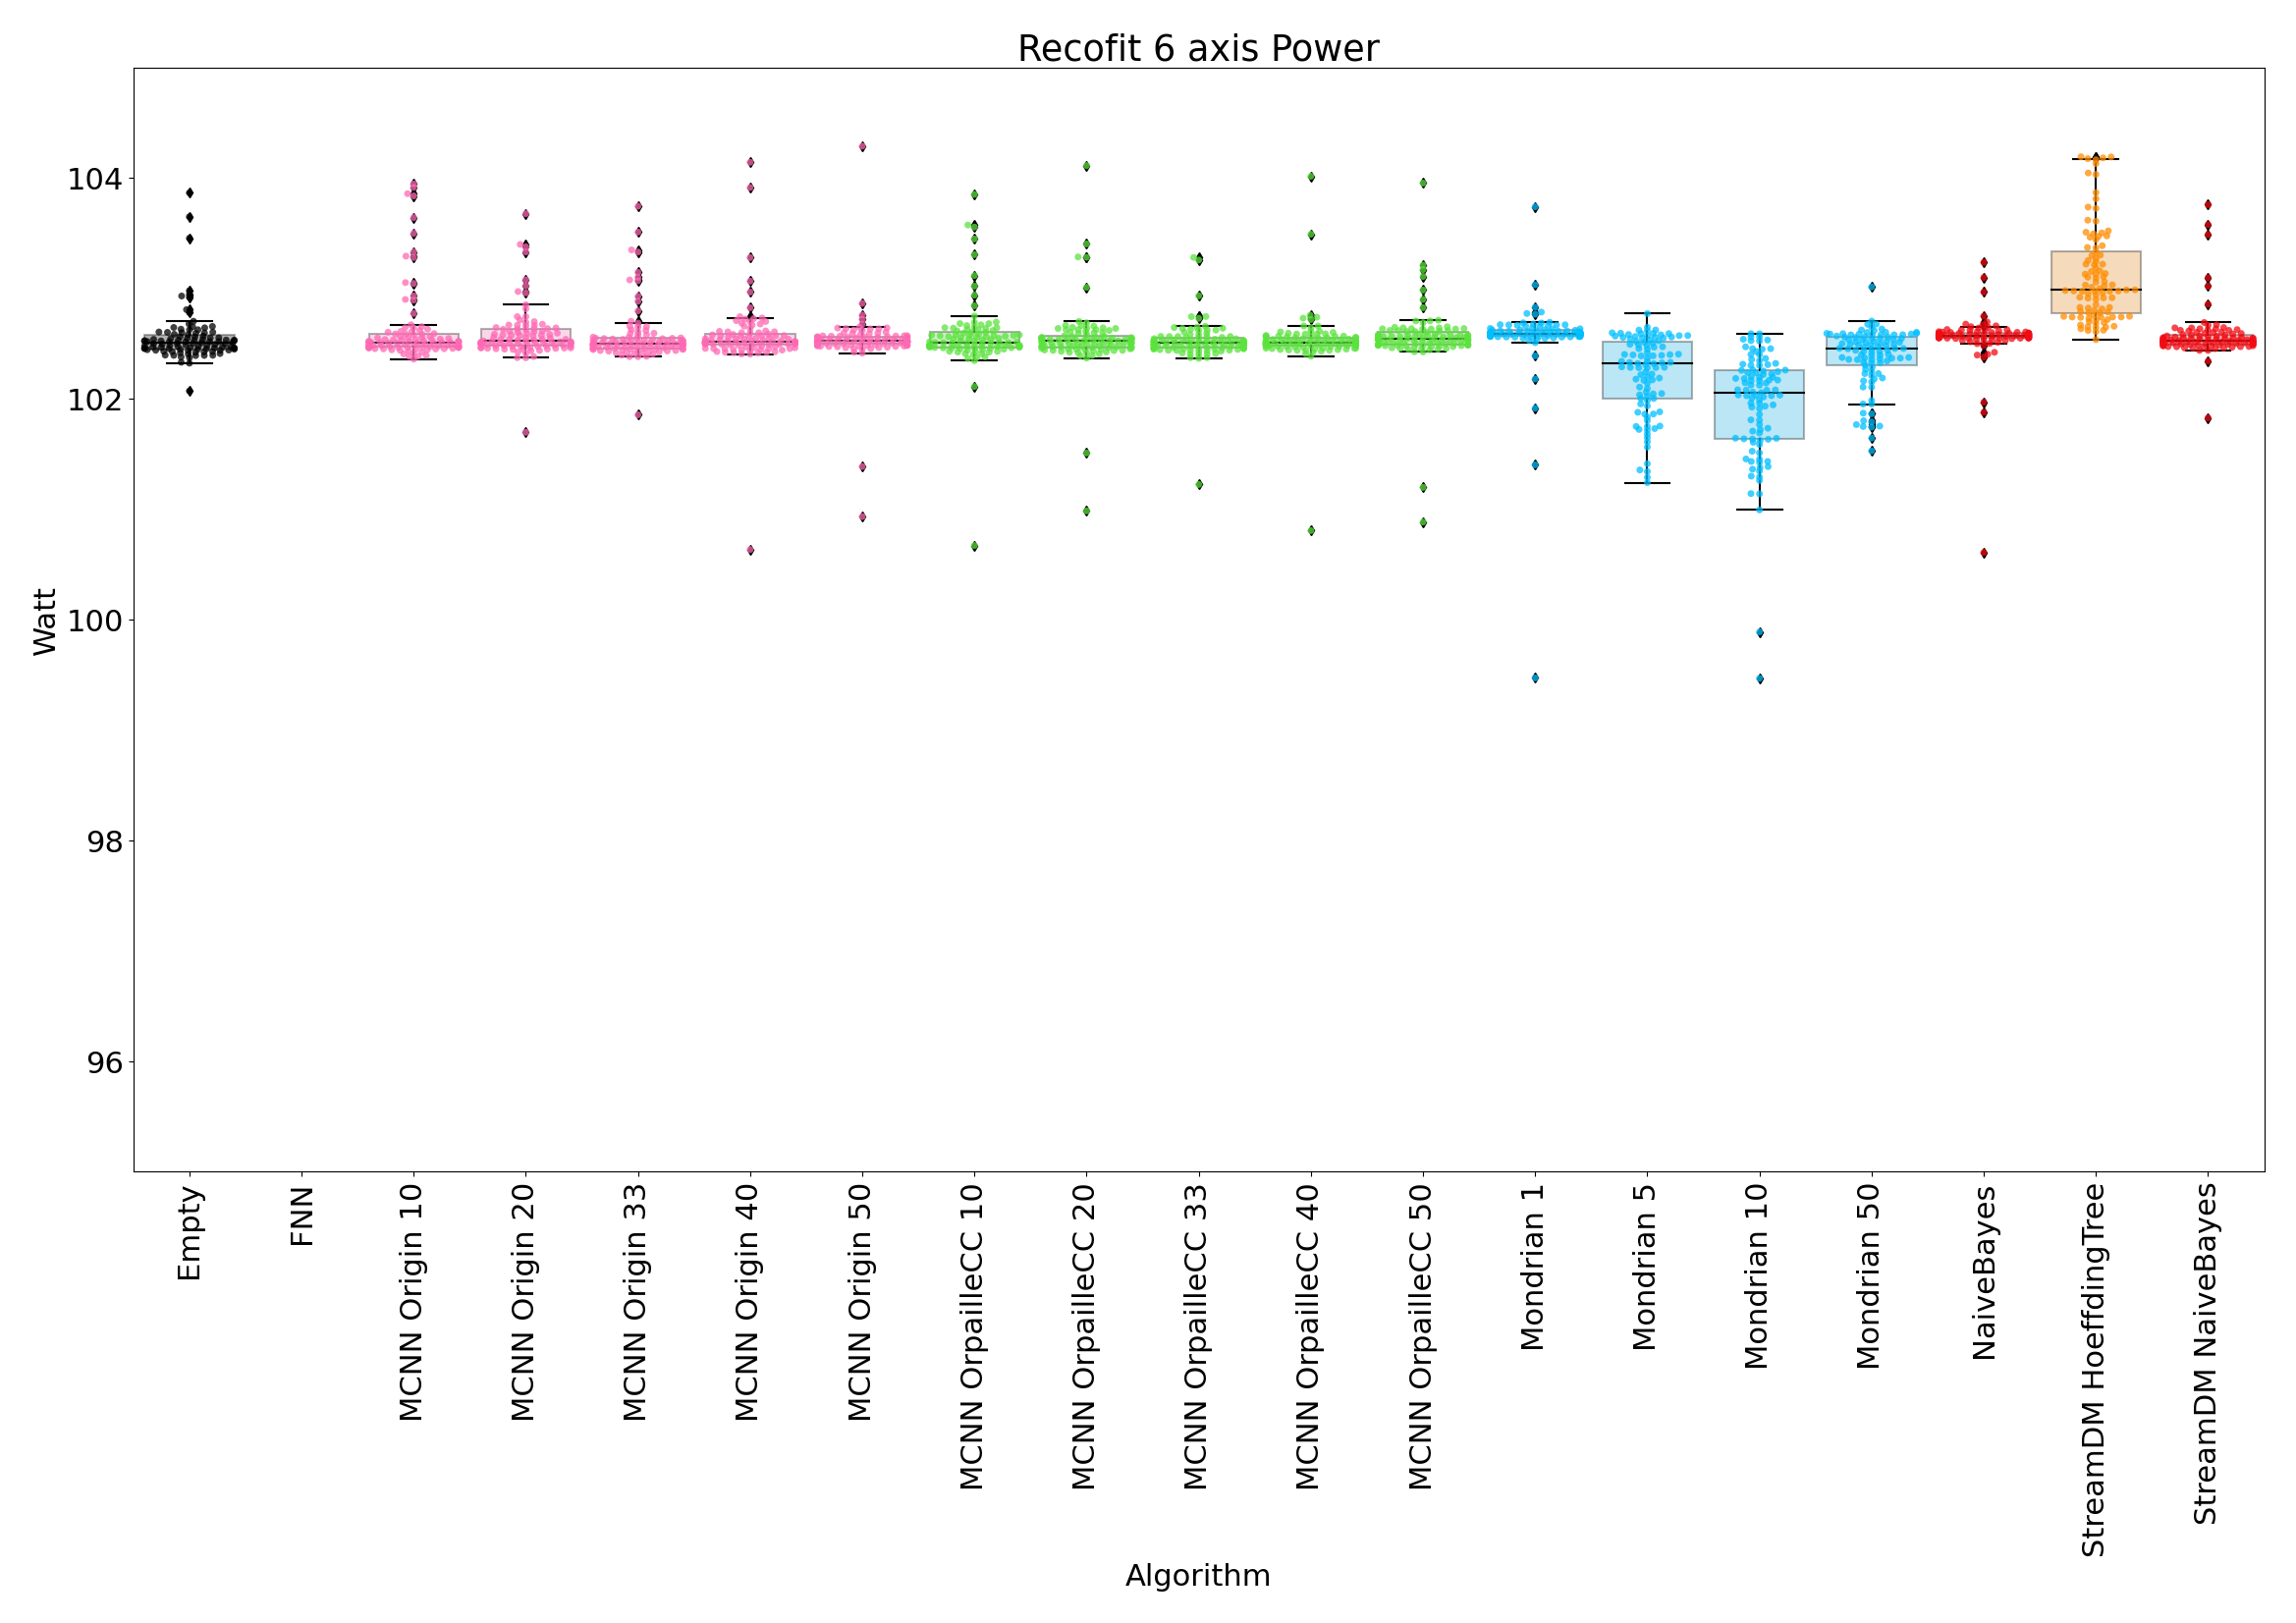
\includegraphics[width=\linewidth]{figures/results/recofit_6_watt.png}
		\caption{\recofitdataset}
		\label{fig:power-recofit}
	\end{subfigure}
	\hfill
	\begin{subfigure}[t]{.49\linewidth}
		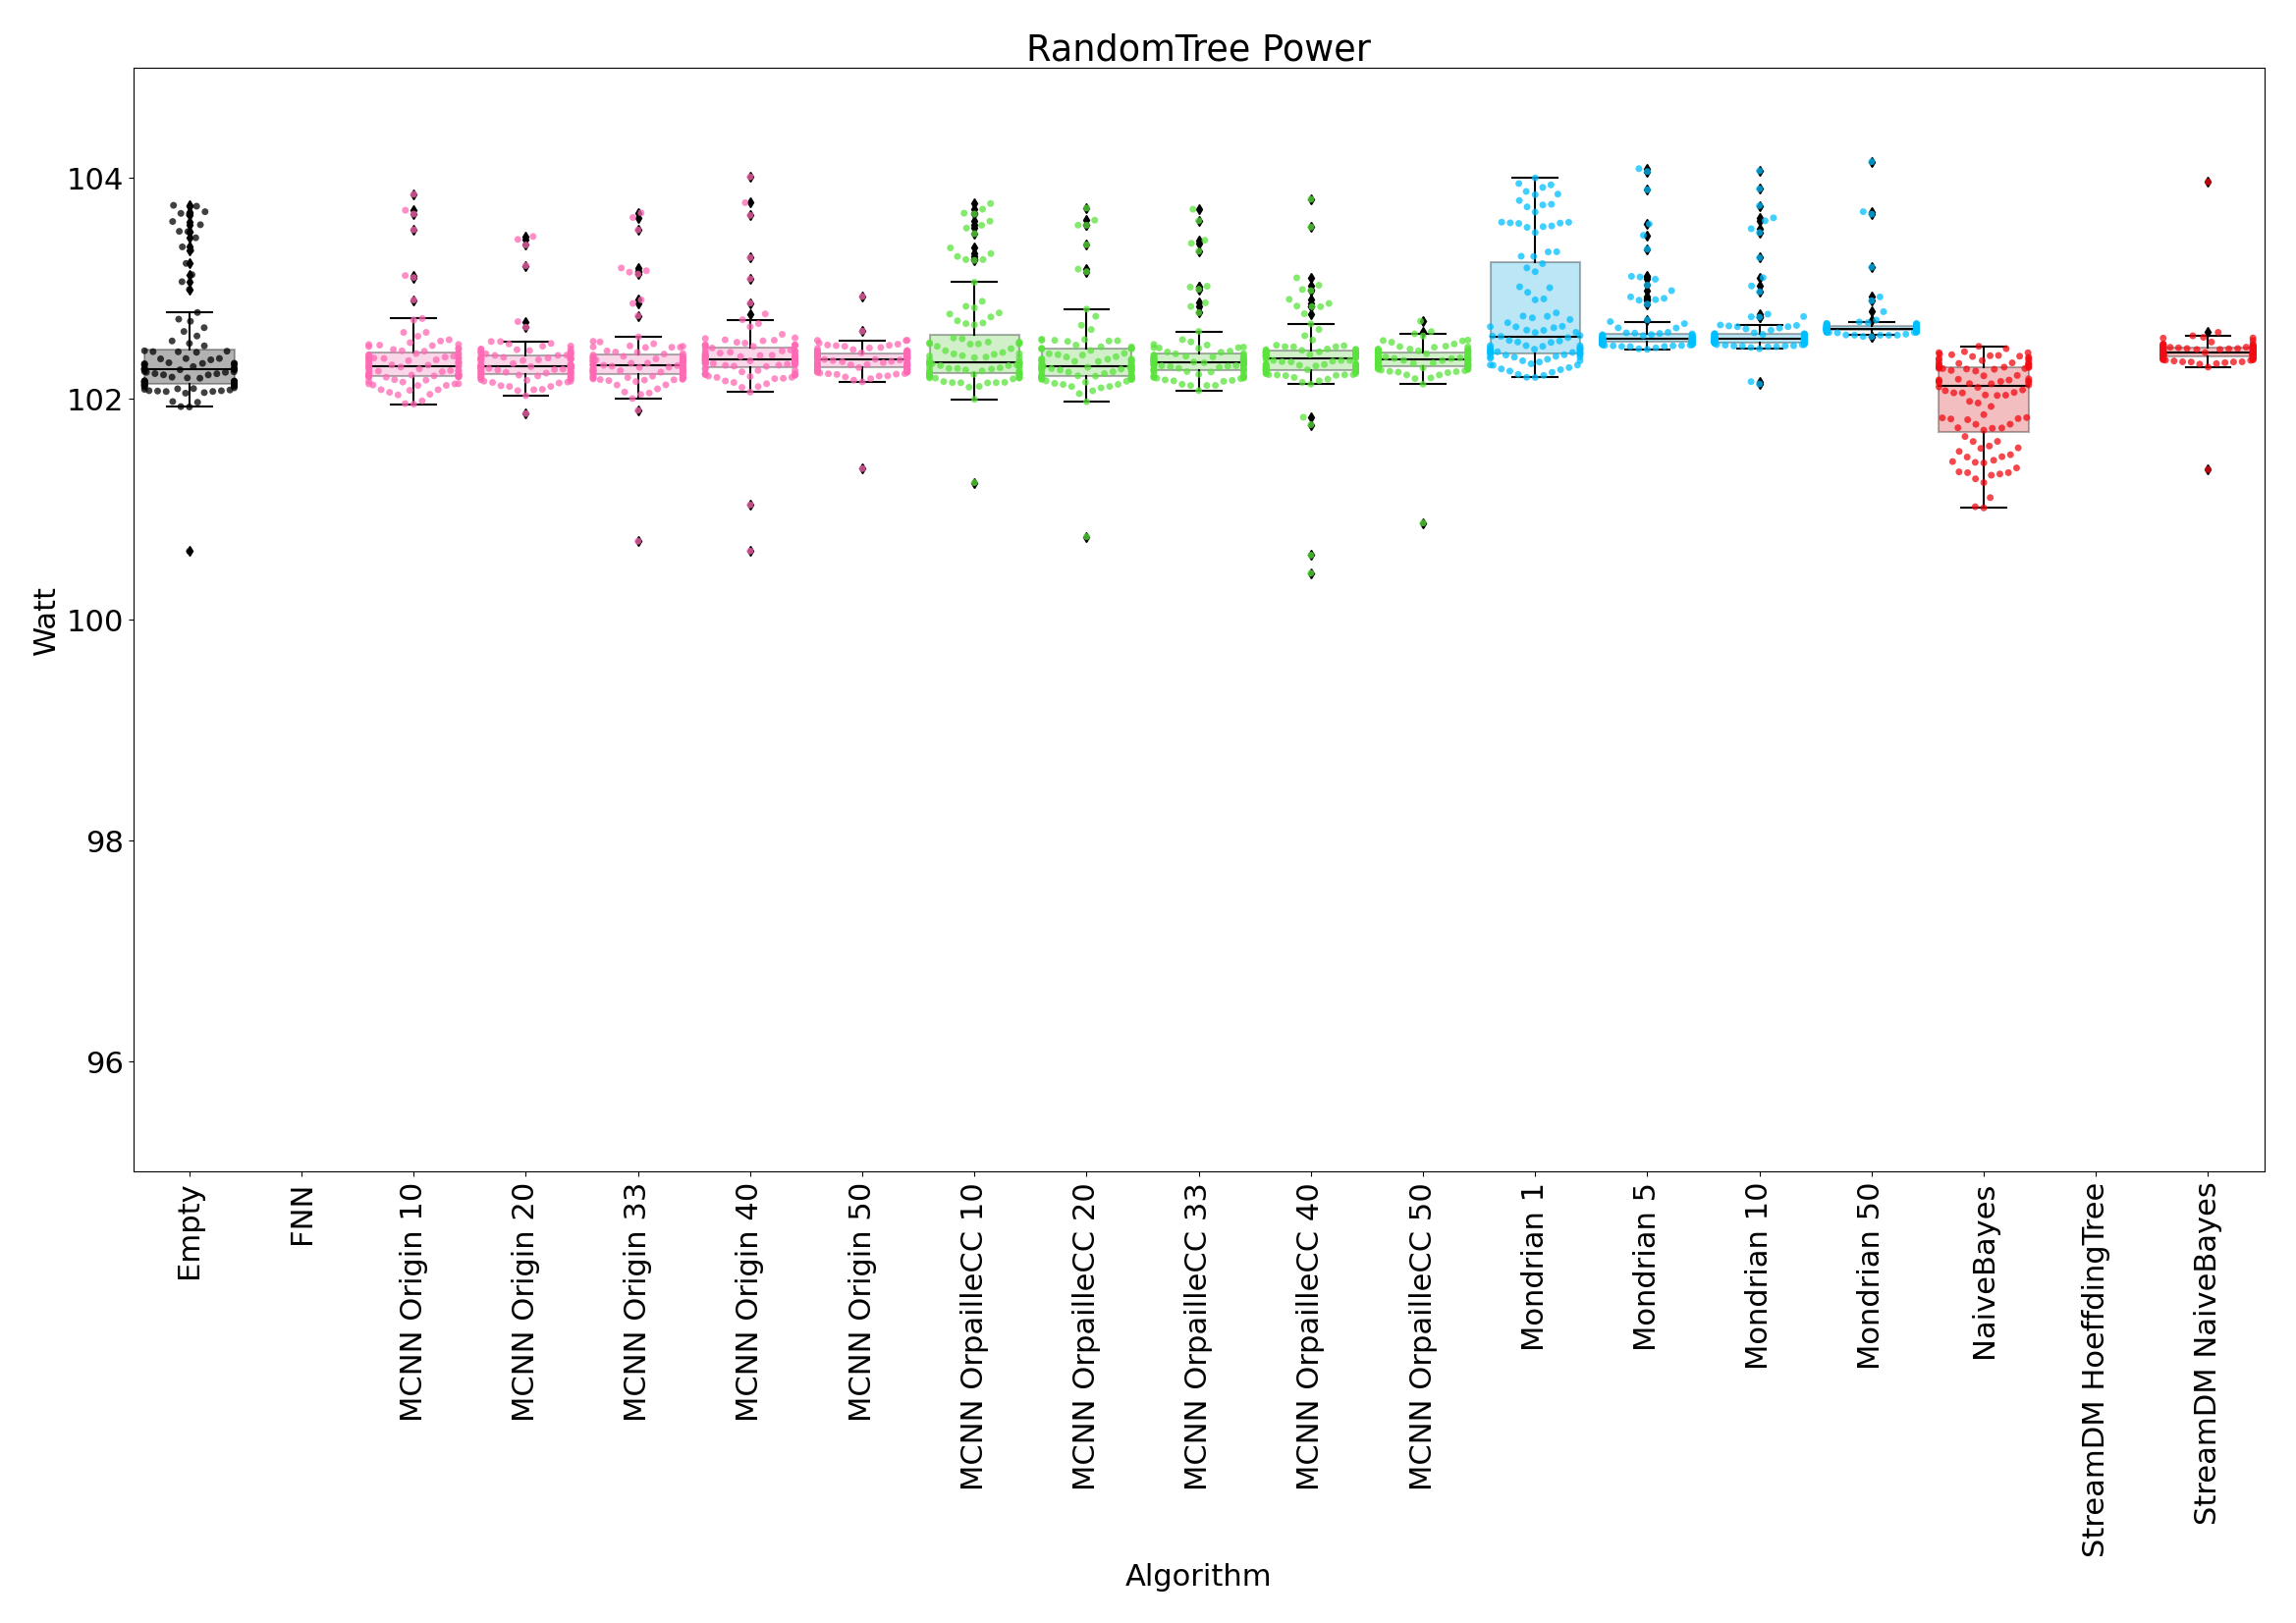
\includegraphics[width=\linewidth]{figures/results/dataset_3_watt.png}
		\caption{RandomTree}
		\label{fig:power-dataset_3}
	\end{subfigure}
	\caption{Power usage for four datasets.}
	\label{fig:power}
\end{figure*}
\subsection{Power}
\label{sec:result-power}
Figure~\ref{fig:power} shows the power usage of each classifier on four
datasets. Since all classifiers exhibit comparable power consumptions, close to
102~W, we decided to show only four of them. Figure~\ref{fig:power-drift} also
shows that the concept drift does not influence the power consumption.

This observation is explainable by two factors. The platform used is too powerful
and it was already working at minimal power. Indeed, to ensure no disturbance
by a background process, we run the classifier on an isolated cluster node with
eight cores. Therefore, the power difference on one core is not noticeable.

Another reason is the dataset size. Indeed, the slowest run is about
10 seconds with 50 Mondrian trees on \recofitdataset dataset.  Such short
execution does not leave the time for the CPU to switch P-states because it
barely warms a core.
\TG{you should explain why your results are still relevant and how they are expected to generalize on 
connected objects.}


\subsection{Runtime}
Figure~\ref{fig:runtime} shows the runtime of classifiers for the two real
datasets. The \mondrianforest is the slowest classifier, in particular for 50
trees. The second slowest classifier is the \hoeffdingtree, with a runtime
comparable to the \mondrianforest with 10 trees. The \hoeffdingtree is followed
by the two \naivebayes implementations, which is not surprising since
\naivebayes classifiers are used in the leaves of the \hoeffdingtree. The \mcnn
classifiers are the fastest ones, with a runtime very close to the empty
classifier. Note that allocating more memory to the \mondrianforest
significatively increase the runtime.

We observe that the runtime of StreamDM's \naivebayes is comparable to
OrpailleCC's. This suggests that the performance of the two libraries is
similar, which justifies our comparision of \hoeffdingtree and \mondrianforest.

\begin{figure*}
	\begin{subfigure}[t]{.49\linewidth}
		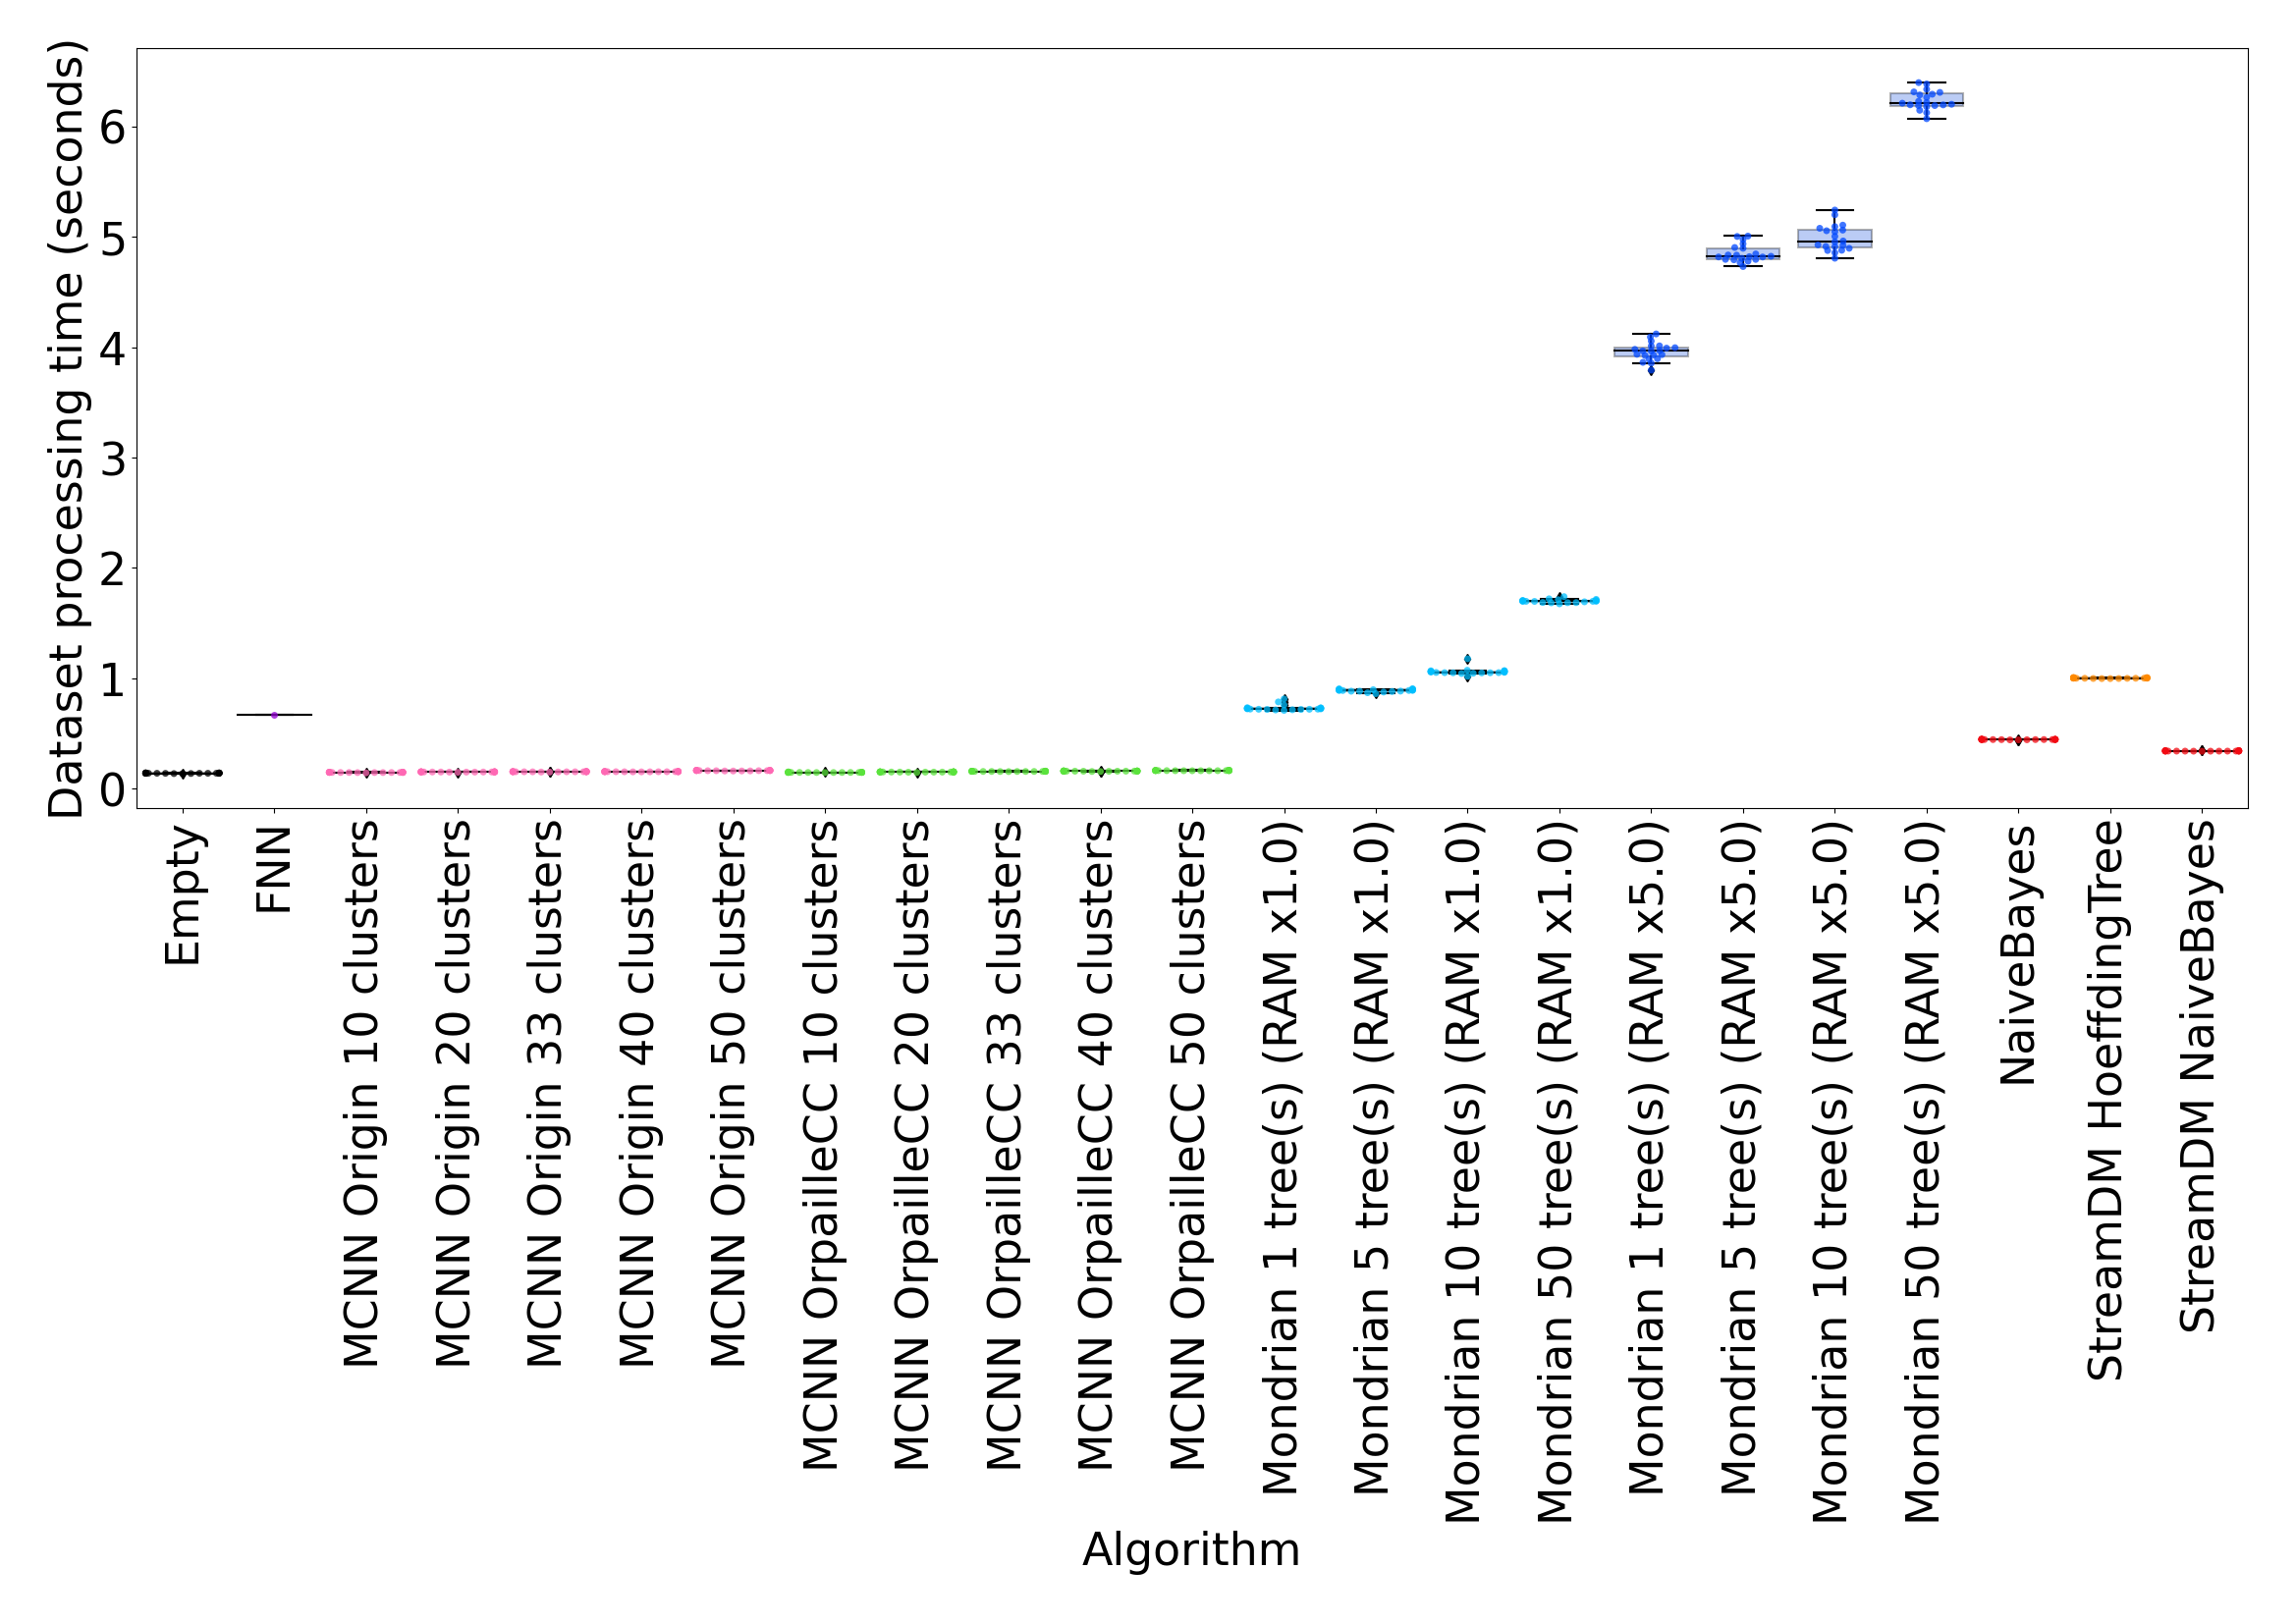
\includegraphics[width=\linewidth]{figures/results/banos_6_runtime.png}
		\caption{\banosdataset}
		\label{fig:runtime-banos}
	\end{subfigure}
	\hfill
	\begin{subfigure}[t]{.49\linewidth}
		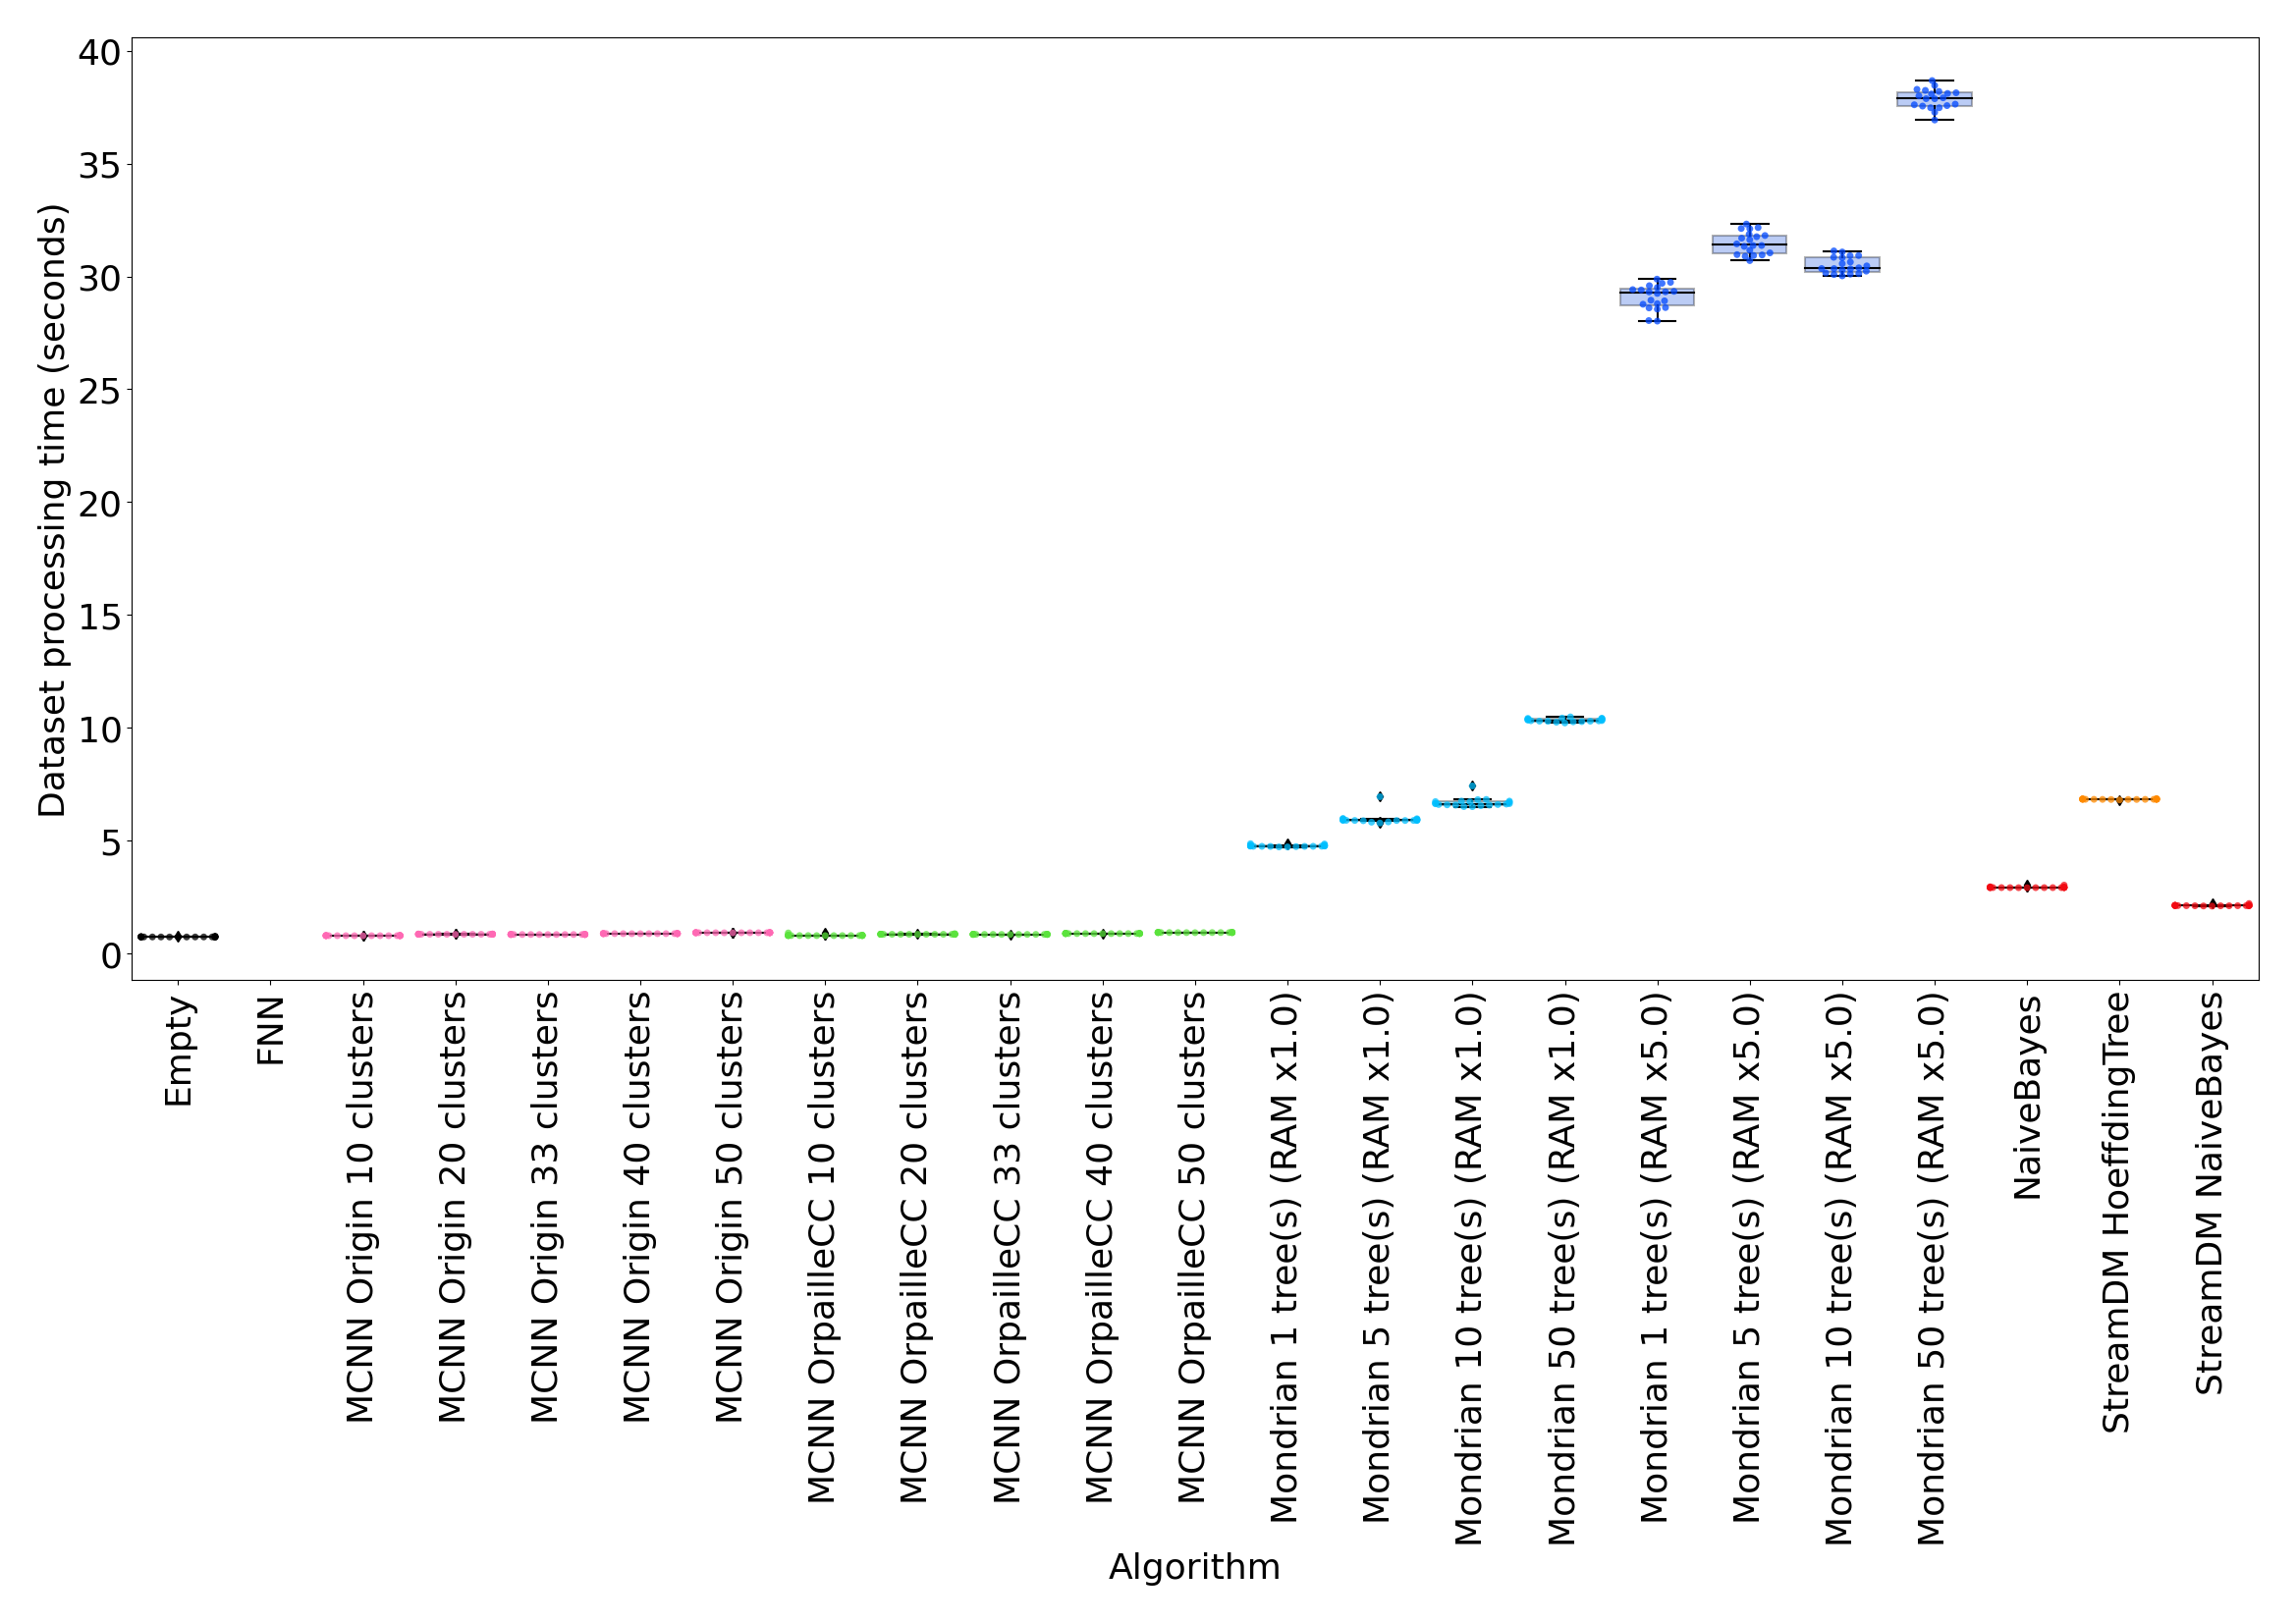
\includegraphics[width=\linewidth]{figures/results/recofit_6_runtime.png}
		\caption{\recofitdataset}
		\label{fig:runtime-recofit}
	\end{subfigure}
	\caption{Runtime with the two real datasets (20 repetitions).}
	\label{fig:runtime}
\end{figure*}

\subsection{Memory}
\label{sec:result-memory}
Figure~\ref{fig:memory} shows the evolution of the memory footprint for the
\banosdataset dataset. Since we observed that \naivebayes memory footprint was
almost indistinguishable from the empty classifier, we used the two \naivebayes
as a baseline for the two libraries. This enables us to remove the 1.2~MB overhead
induced by StreamDM.

We observe that the memory footprints of the \mondrianforest and the
\hoeffdingtree are significatively higher while the \mcnns and the \naivebayes are
close to zero~KB.
Overall, memory footprints are similar across datasets, due to the
fact that most algorithms follow a bounded memory policy or have a constant
space complexity.  The only exception is the \hoeffdingtree that constantly
selects new splits depending on new data points. The \mondrianforest has the
same behavior but the OrpailleCC implementation includes a memory bound, which
makes its memory footprint constant. Note that the concept drift does not
increase the memory footprint of the \hoeffdingtree.

\begin{figure}
	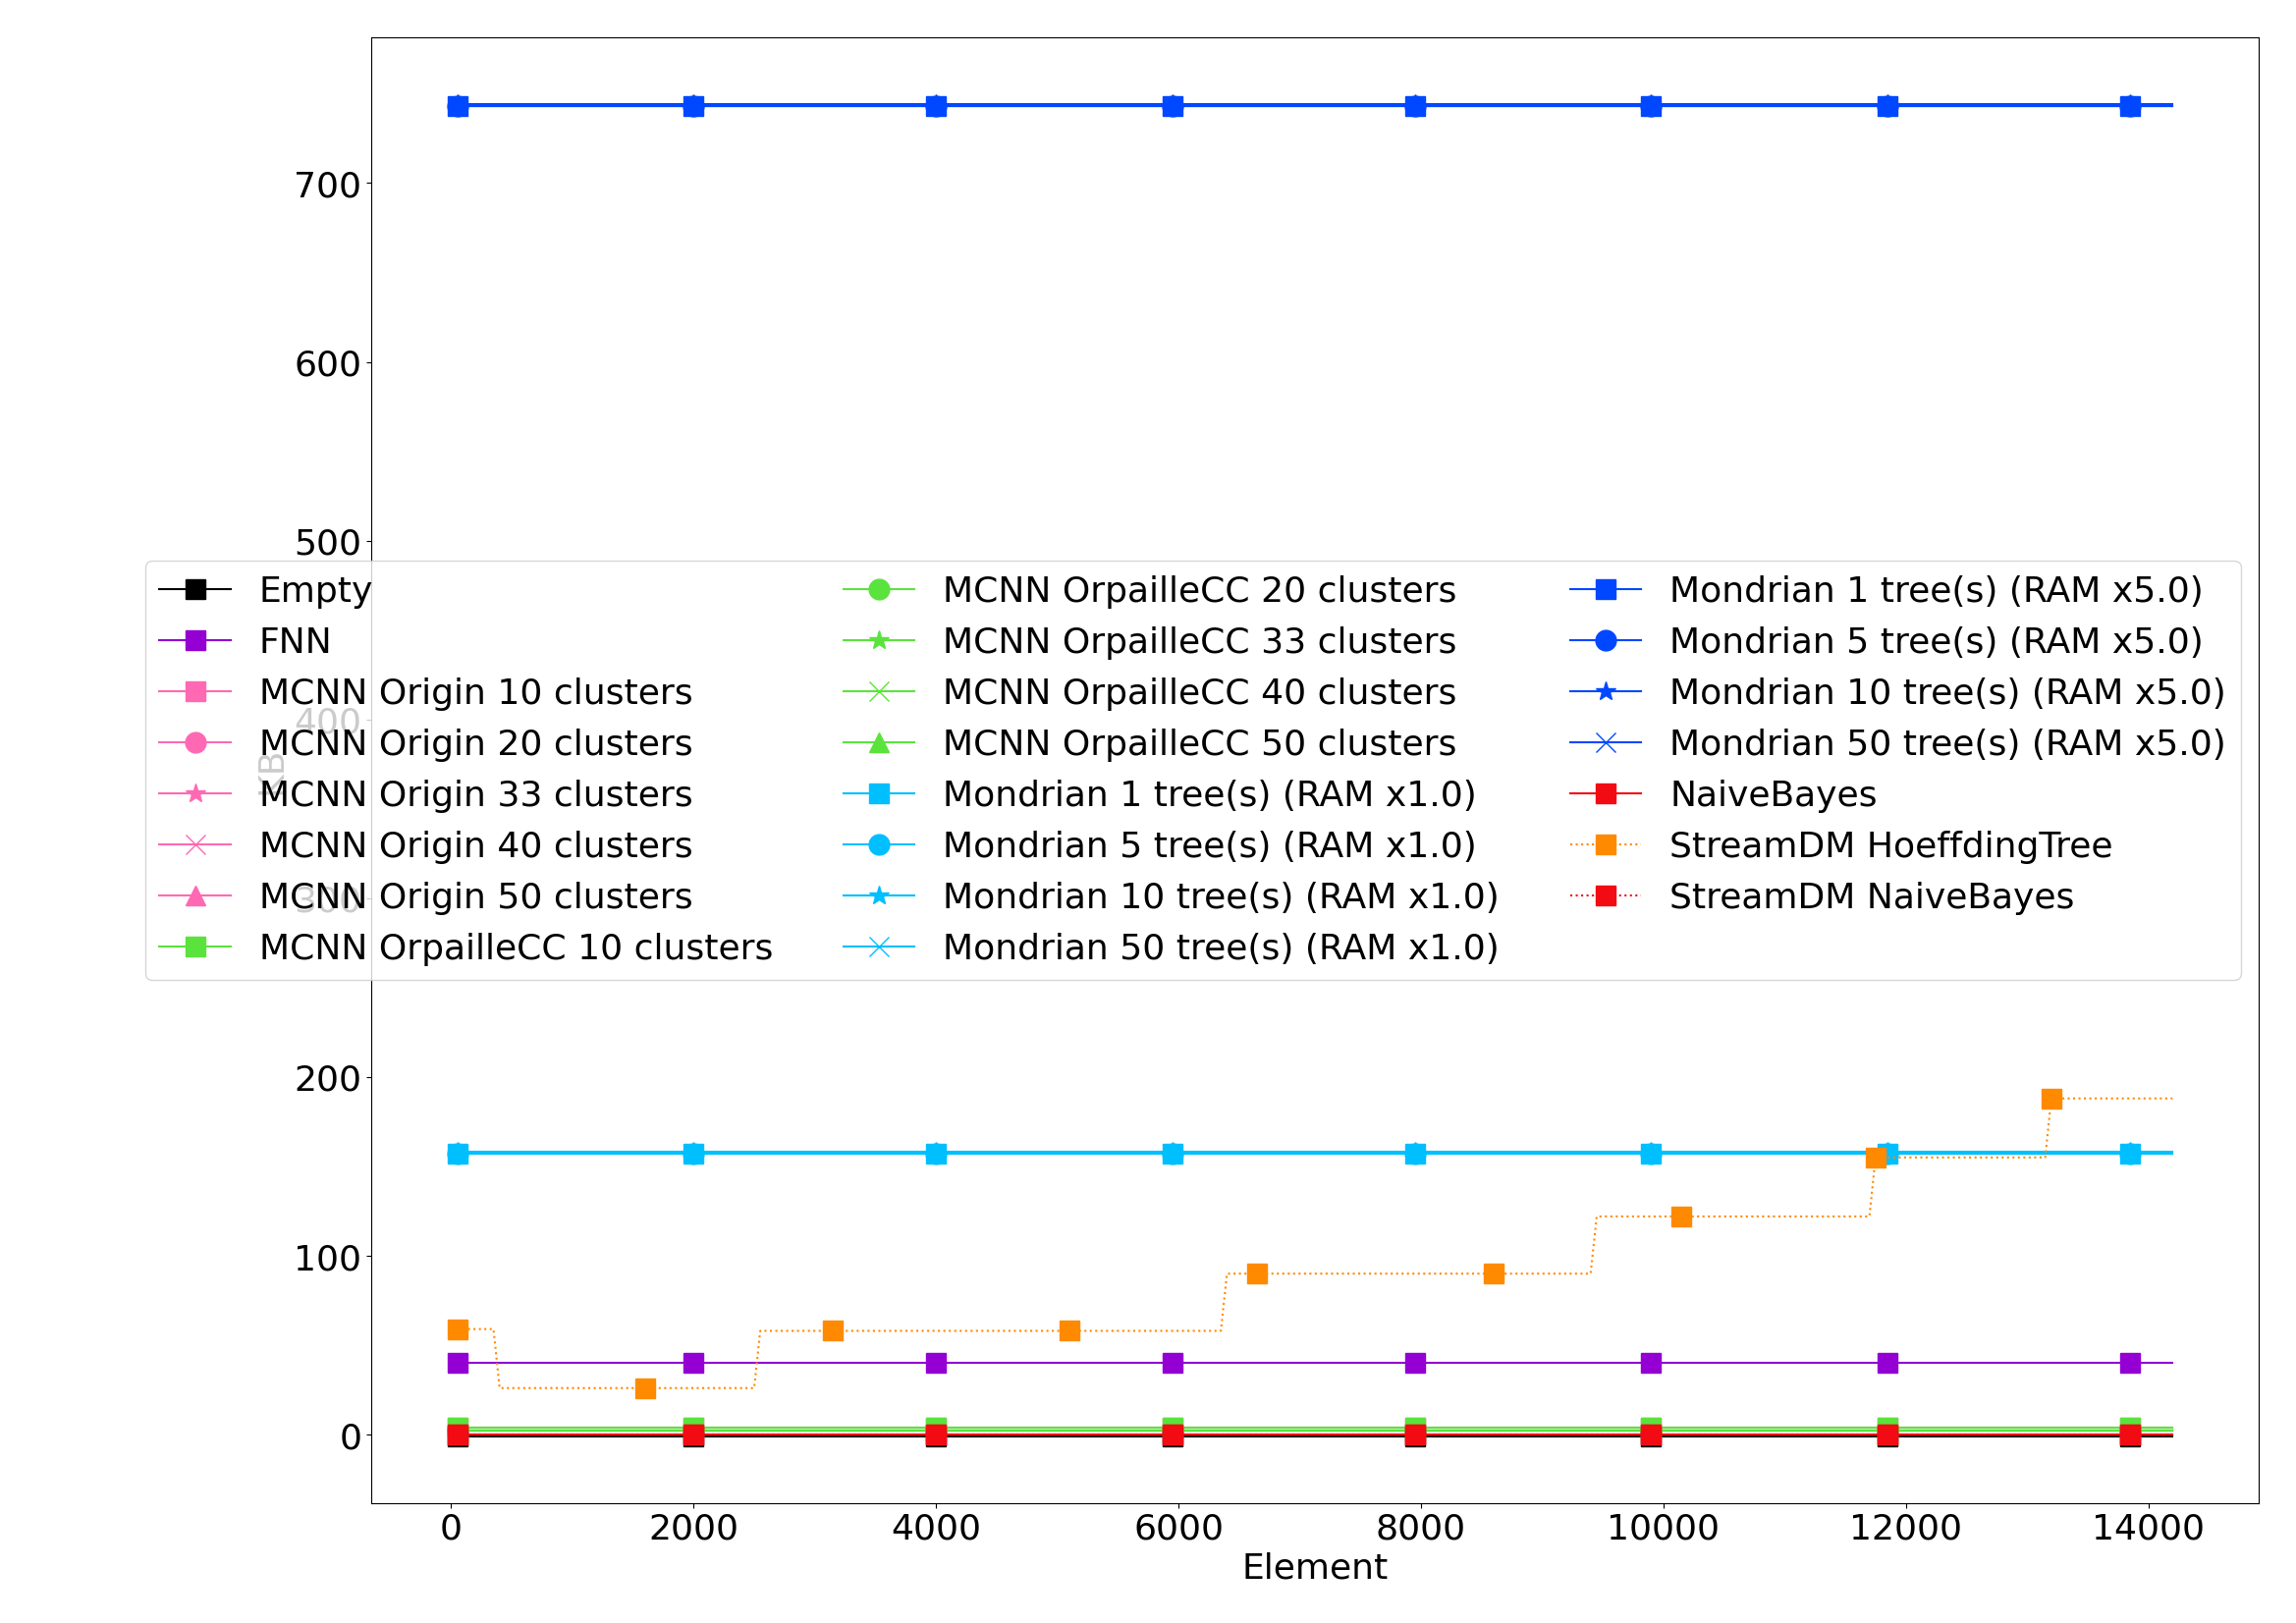
\includegraphics[width=\linewidth]{figures/results/banos_6_memory.png}
	\caption{Memory footprint of the classifiers relatively to the empty
	classifier, measured on the \banosdataset dataset. The memory footprint of the empty
	classifier is slightly above 3.439MB.}
	\label{fig:memory}
\end{figure}


\subsection{Micro-Cluster Nearest Neighbor Hyperparameters}

Figure~\ref{fig:mcnn-tuning-error} shows the impact of the error threshold
in the \mcnn classifiers with different cluster counts. The error
threshold of \mcnn has little impact on the classification performance. For
20 and 40 clusters, the best-performing threshold is either 2 or 4, meaning
that a cluster may do 2 or 4 errors before being split. For 10 clusters,
all error thresholds perform equally.

\begin{figure}
	 \begin{subfigure}[b]{0.49\textwidth}
		 \centering
		 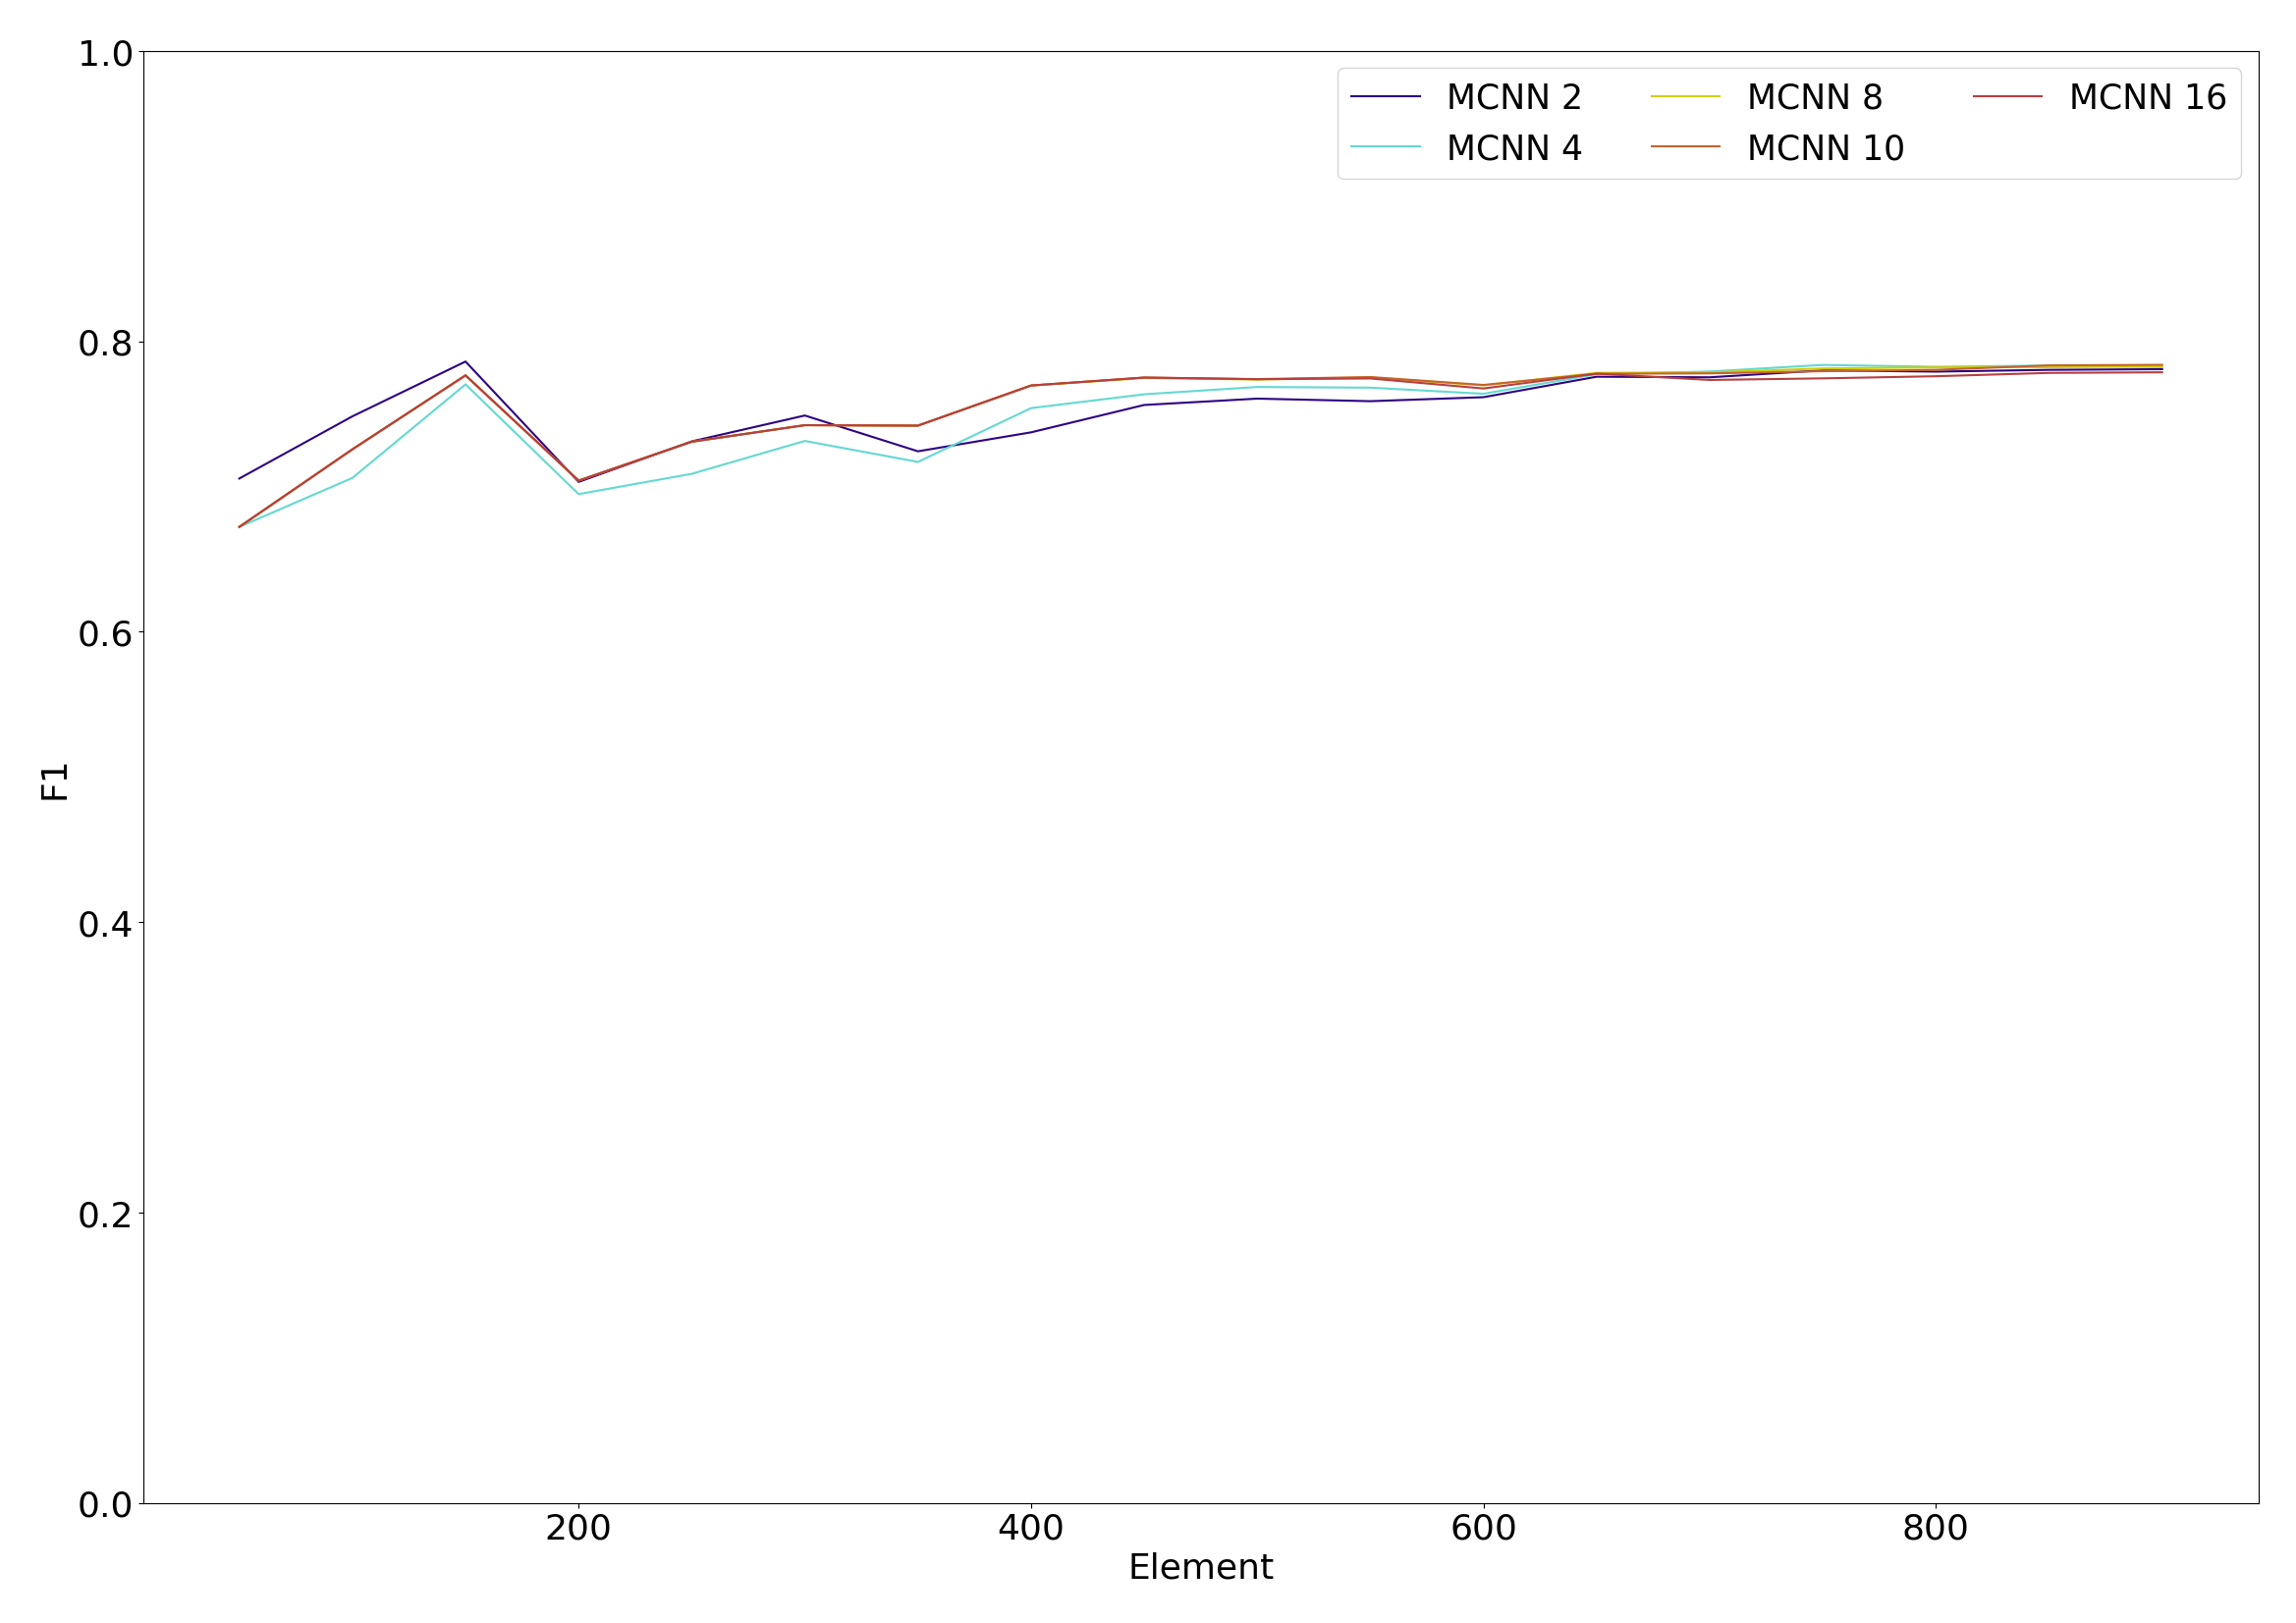
\includegraphics[width=\linewidth]{figures/calibration_mcnn_40.png}
		 \caption{40 clusters}
	 \end{subfigure}
	 \begin{subfigure}[b]{0.49\textwidth}
		 \centering
		 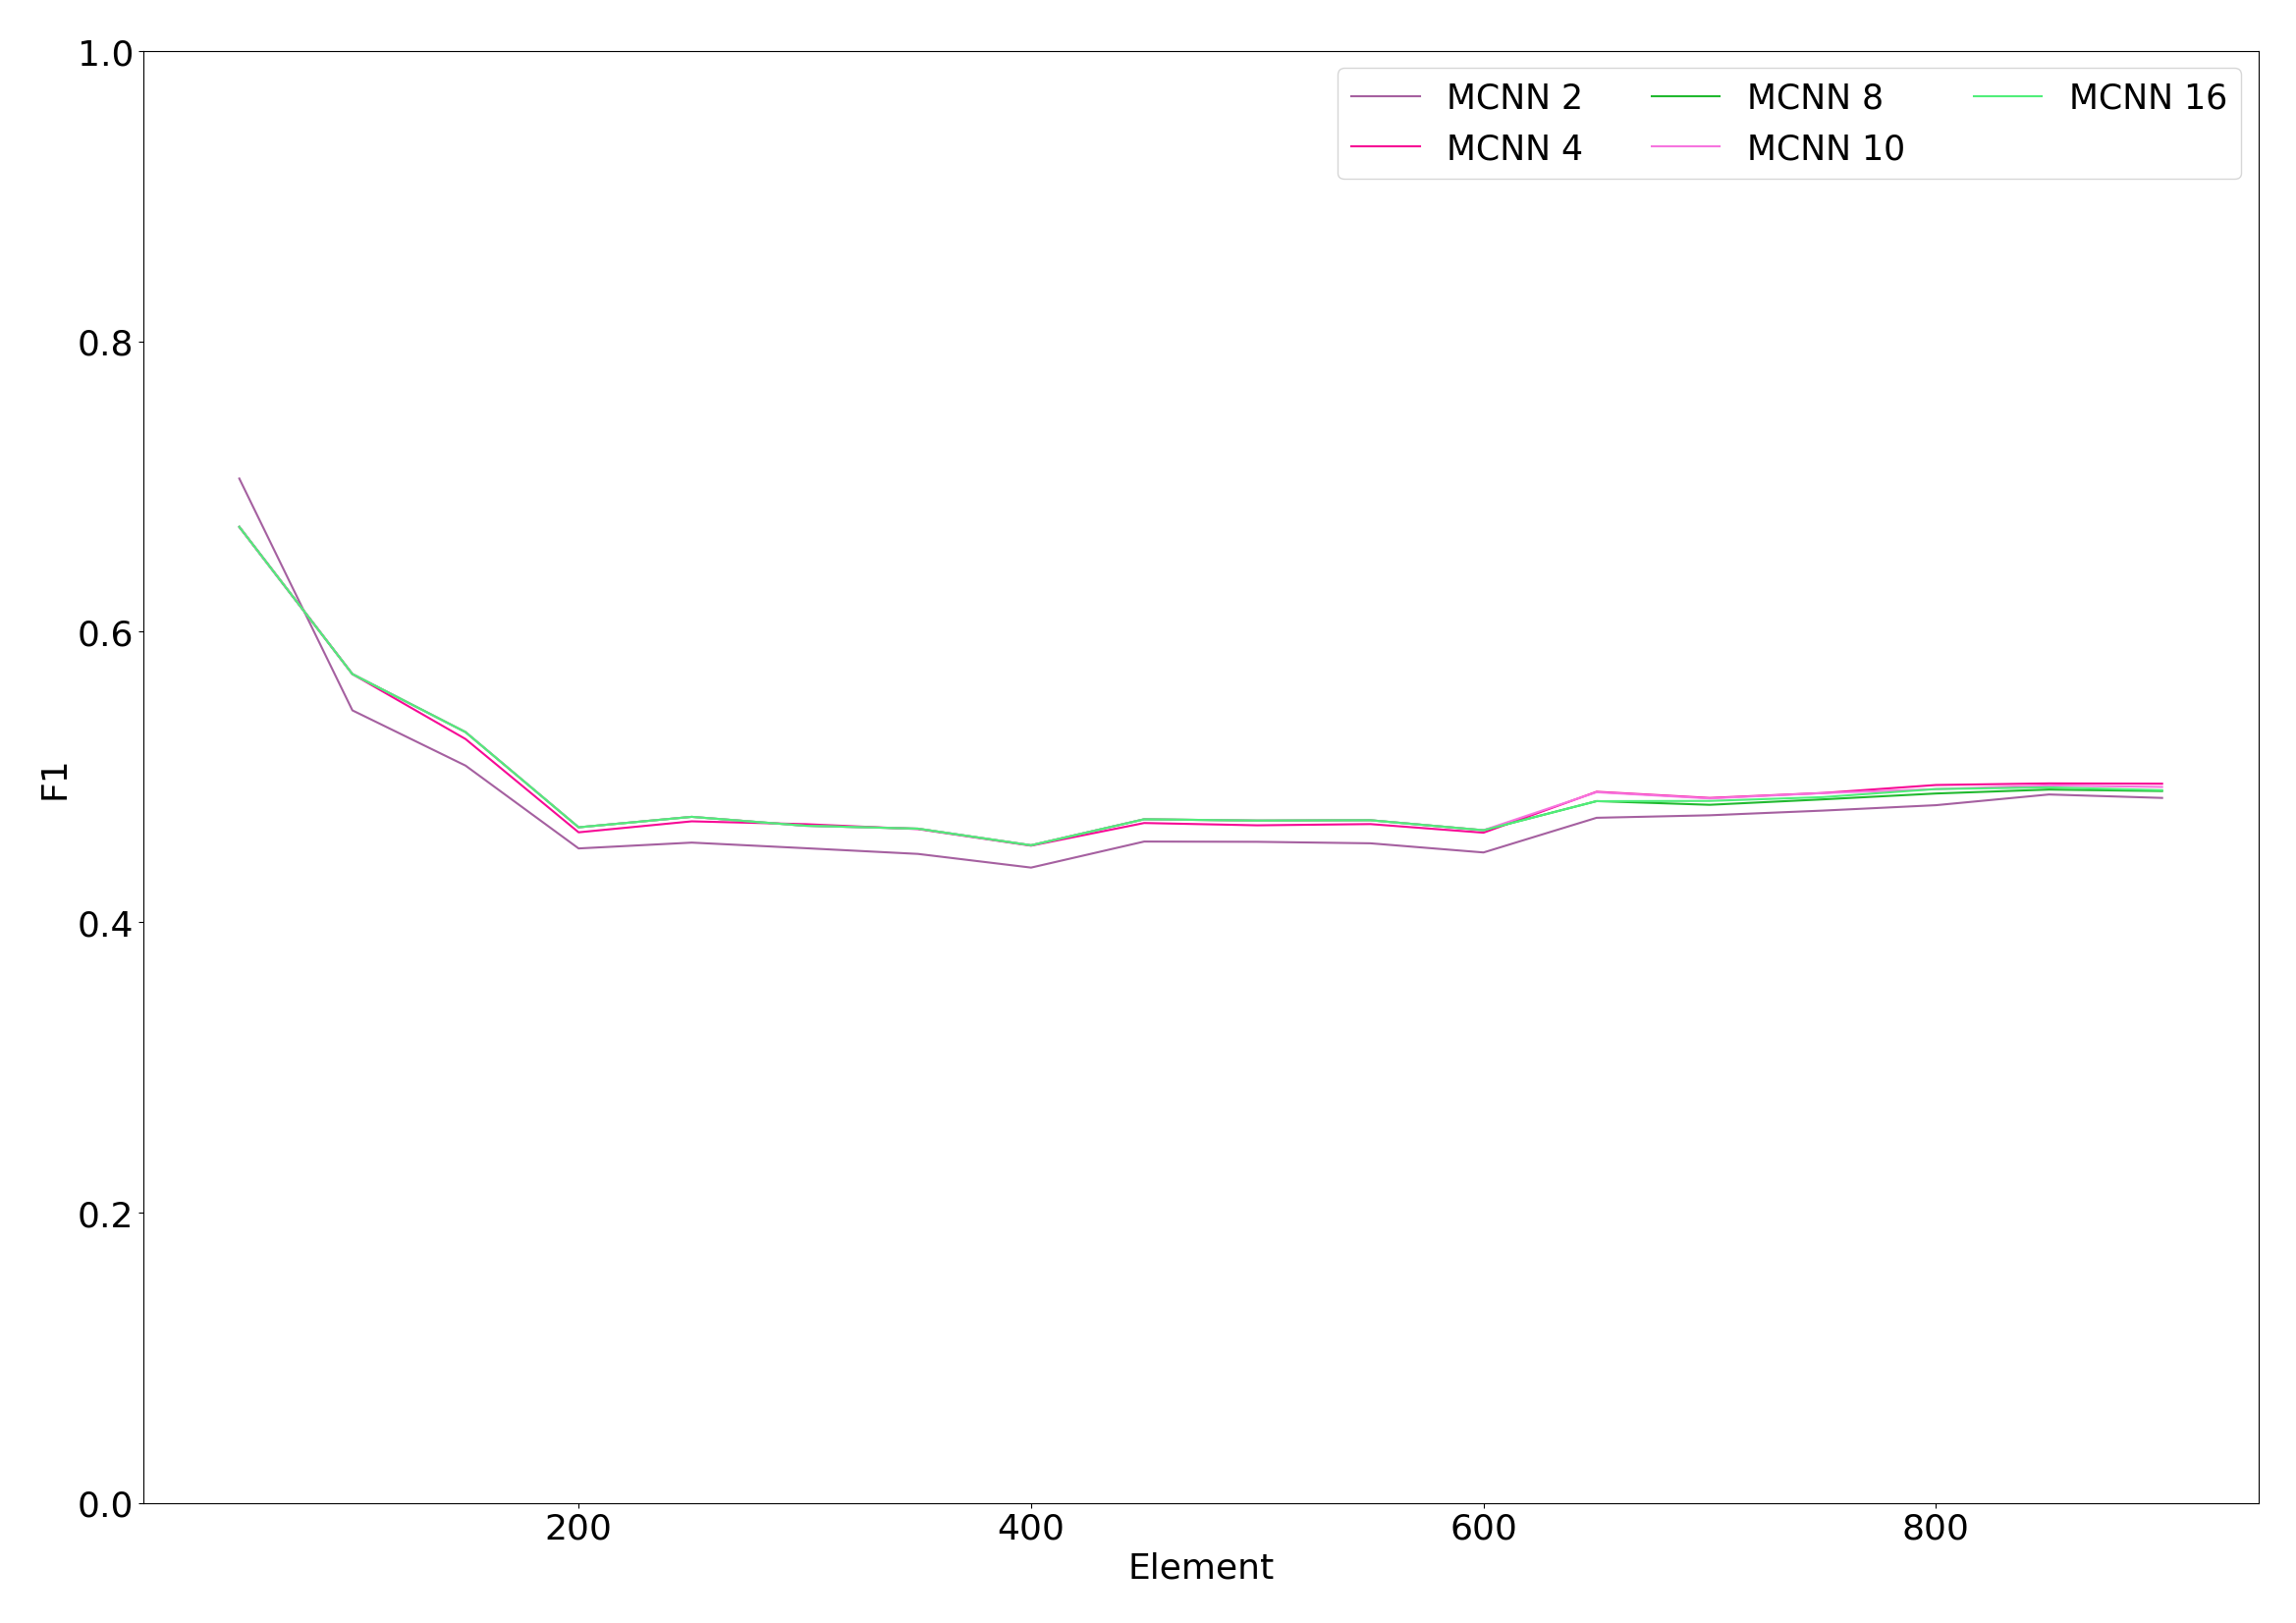
\includegraphics[width=\linewidth]{figures/calibration_mcnn_20.png}
		 \caption{20 clusters}
	 \end{subfigure}
	 \begin{subfigure}[b]{0.49\textwidth}
		 \centering
		 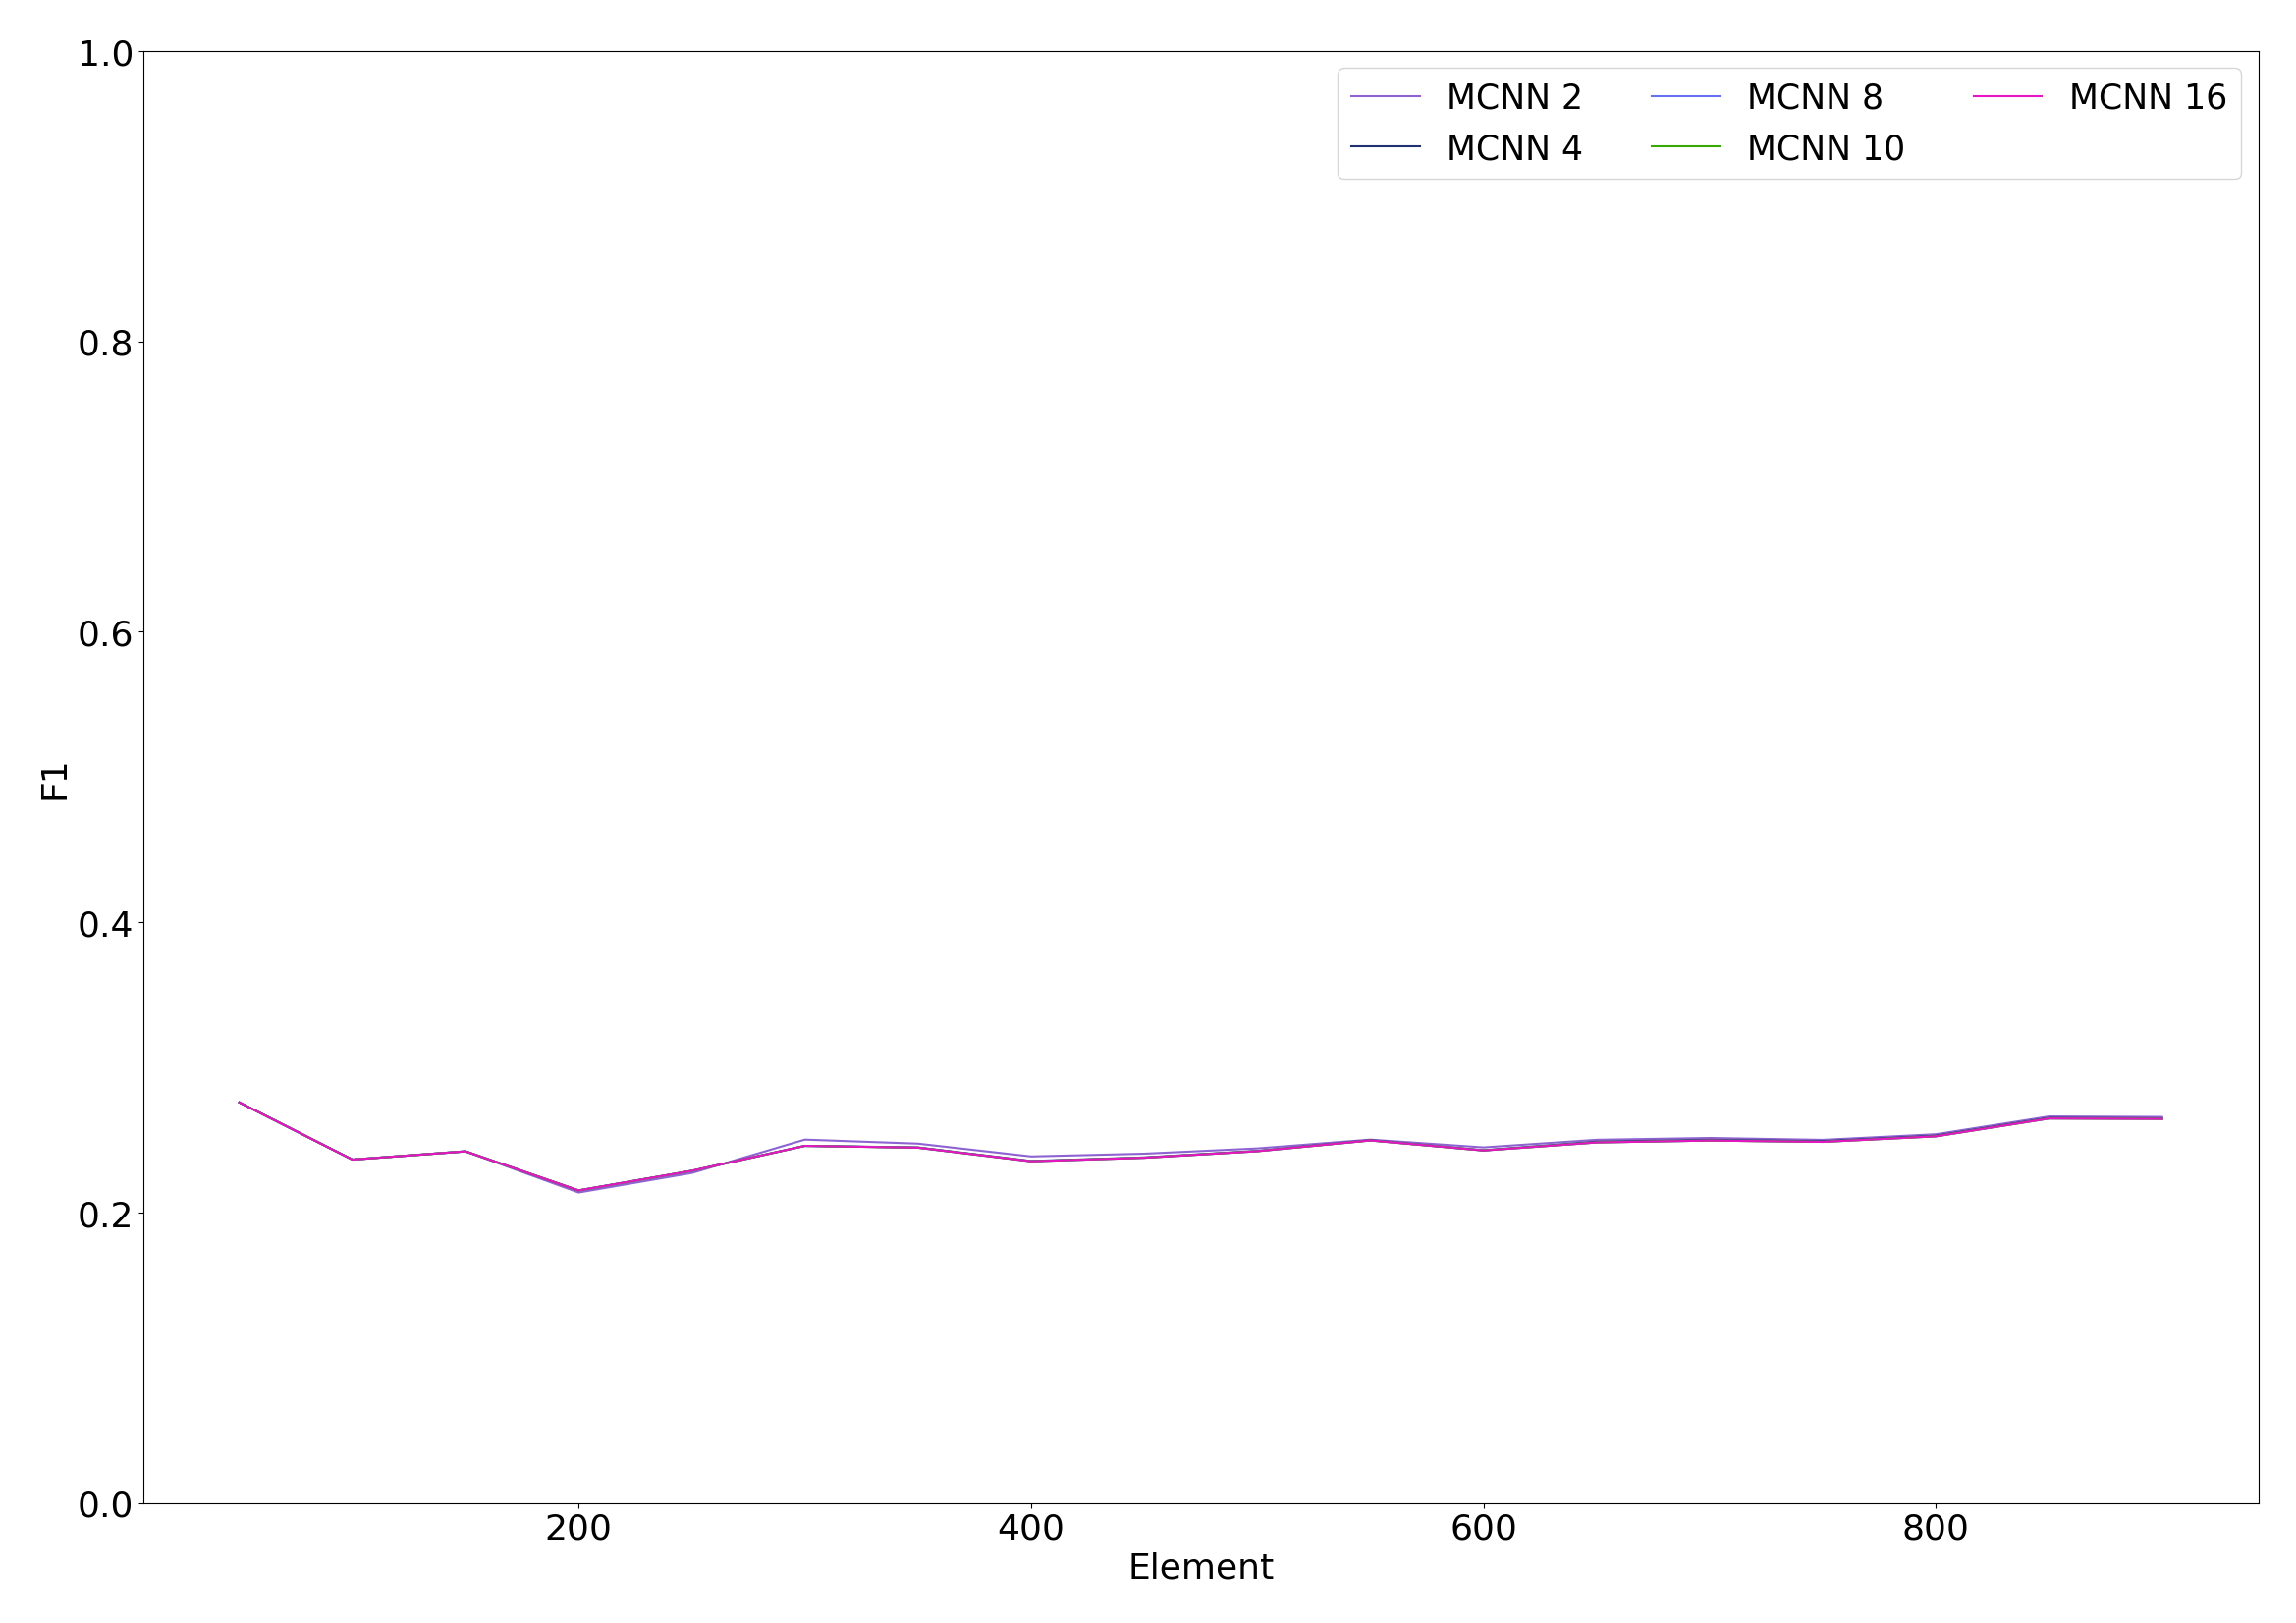
\includegraphics[width=\linewidth]{figures/calibration_mcnn_10.png}
		 \caption{10 clusters}
	 \end{subfigure}
	\caption{Error threshold tuning of \mcnn with first subject of \banosdataset dataset.}
	\label{fig:mcnn-tuning-error}
\end{figure}

\subsection{\mondrianforest Hyperparameters}

Figure~\ref{fig:mondrian-tuning} shows the impact of the \mondrianforest hyperparameters on
the classification performance. 

The base count hyperparameter (Figure~\ref{fig:mondrian-base-count}) has a
very substantial impact on classification performance; the smallest value
(0.0) results in the best performance. On the contrary, the
budget hyperparameter (Figure~\ref{fig:mondrian-budget}) only has a
moderate impact on classification; the best value is 0.2. Finally, the discount hyperparameter
(Figure~\ref{fig:mondrian-discount}) has a negligible impact on the
performance; the best-performing value is 0.1.

\begin{figure}
	 \centering
	 \begin{subfigure}[b]{0.49\textwidth}
		\centering
		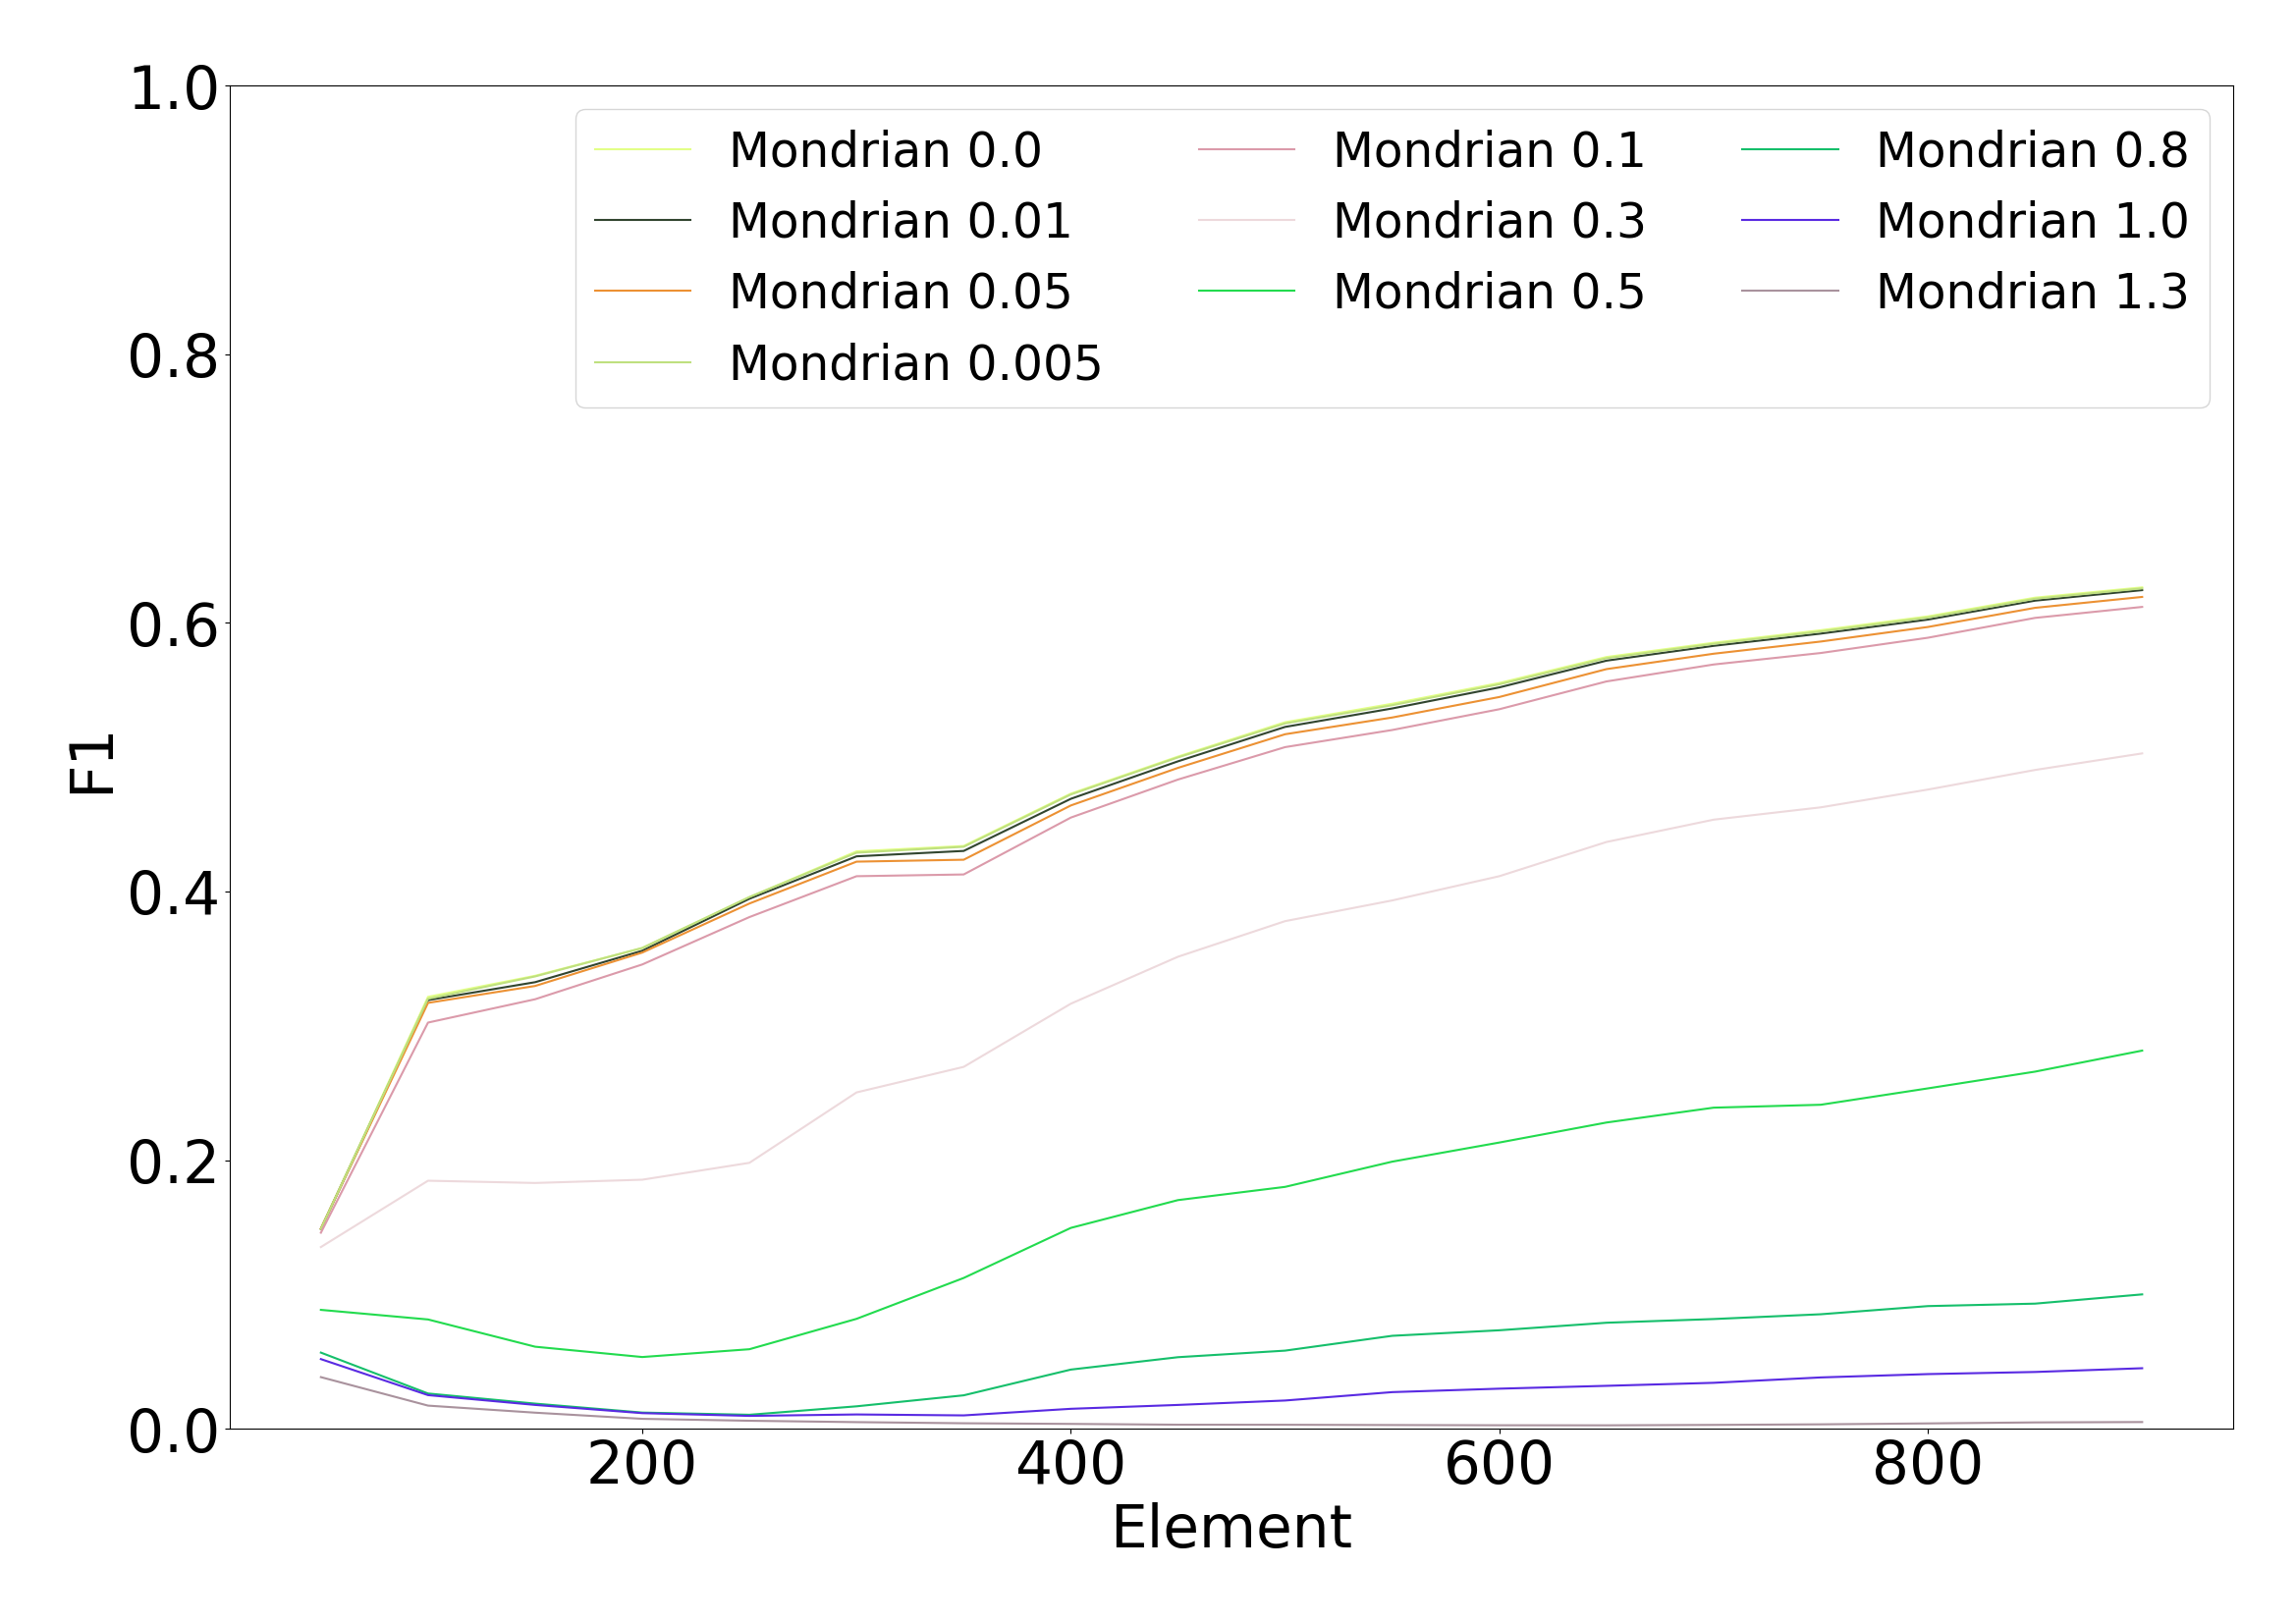
\includegraphics[width=\textwidth]{figures/calibration_mondrian_base.png}
		\caption{Impact of the base count with 10 trees, a budget of $1.0$, and a discount factor of $0.2$.} 
		\label{fig:mondrian-base-count}
	\end{subfigure}
	\hfill
	 \begin{subfigure}[b]{0.49\textwidth}
		 \centering
		 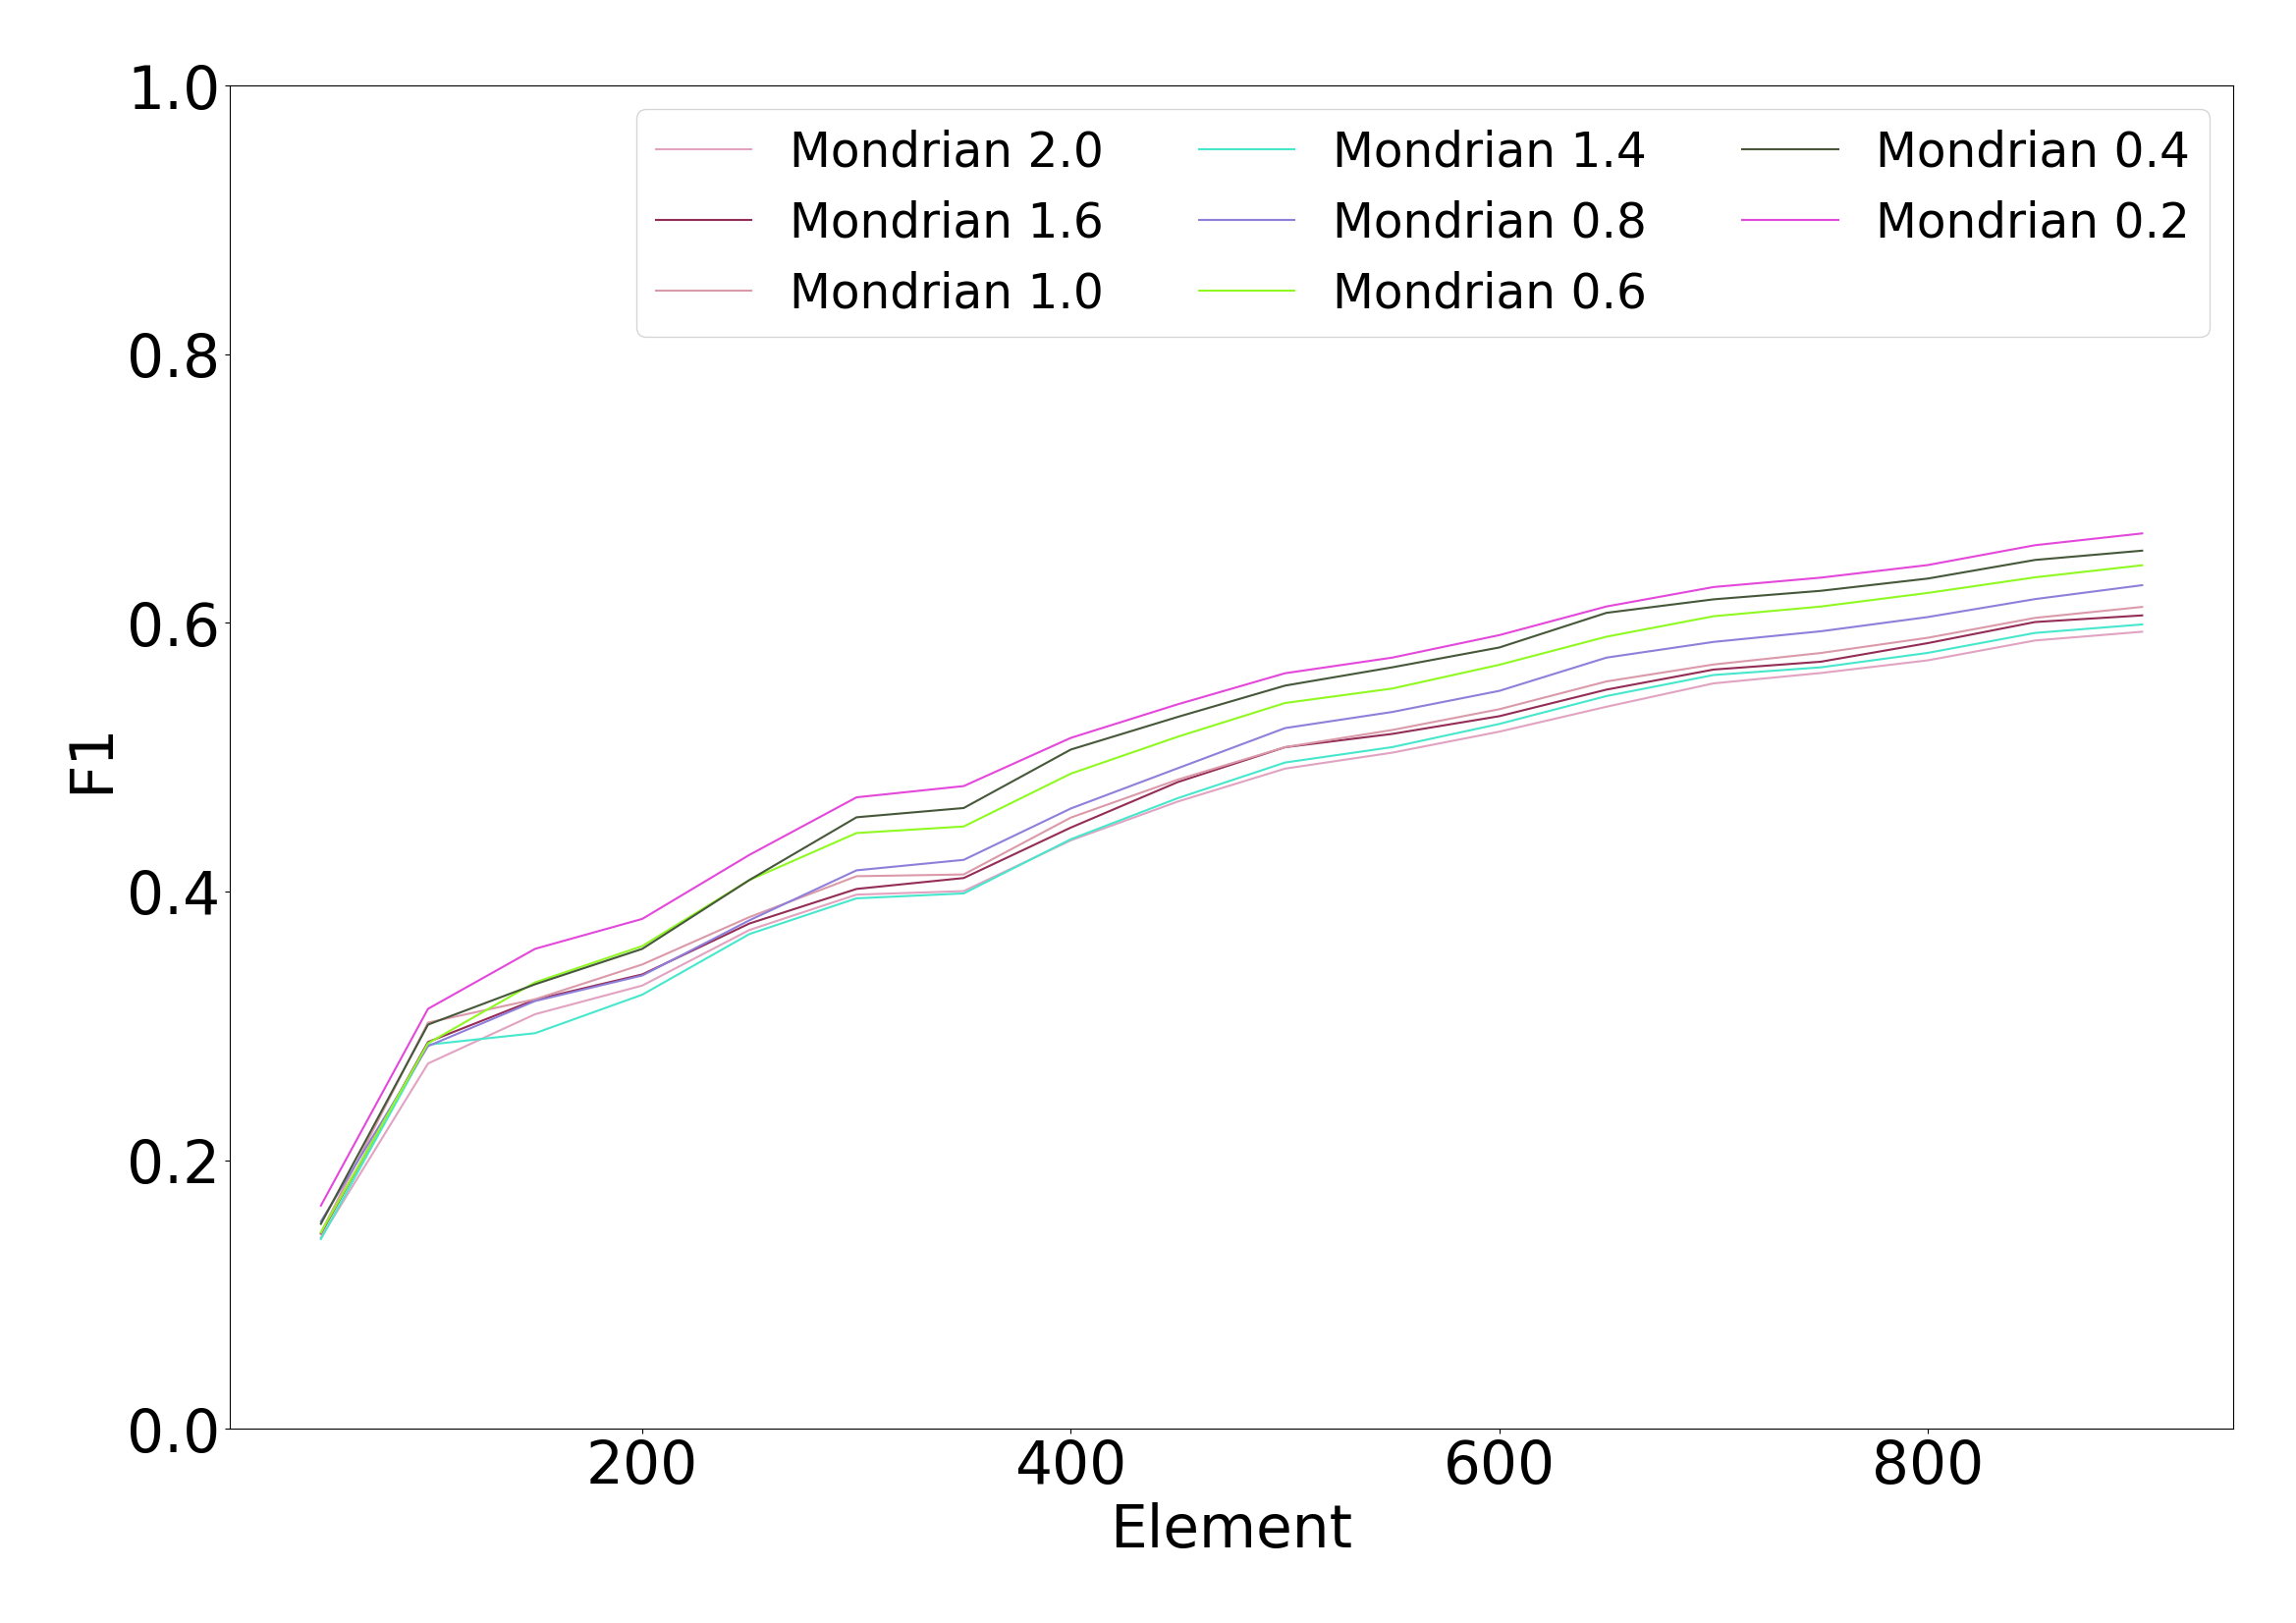
\includegraphics[width=\textwidth]{figures/calibration_mondrian_lifetime.png}
		 \caption{Impact of the budget with 10 trees, a base count of $0.1$, and discount factor of $0.2$.}
		 \label{fig:mondrian-budget}
	 \end{subfigure}
	 \hfill
	 \begin{subfigure}[b]{0.49\textwidth}
		 \centering
		 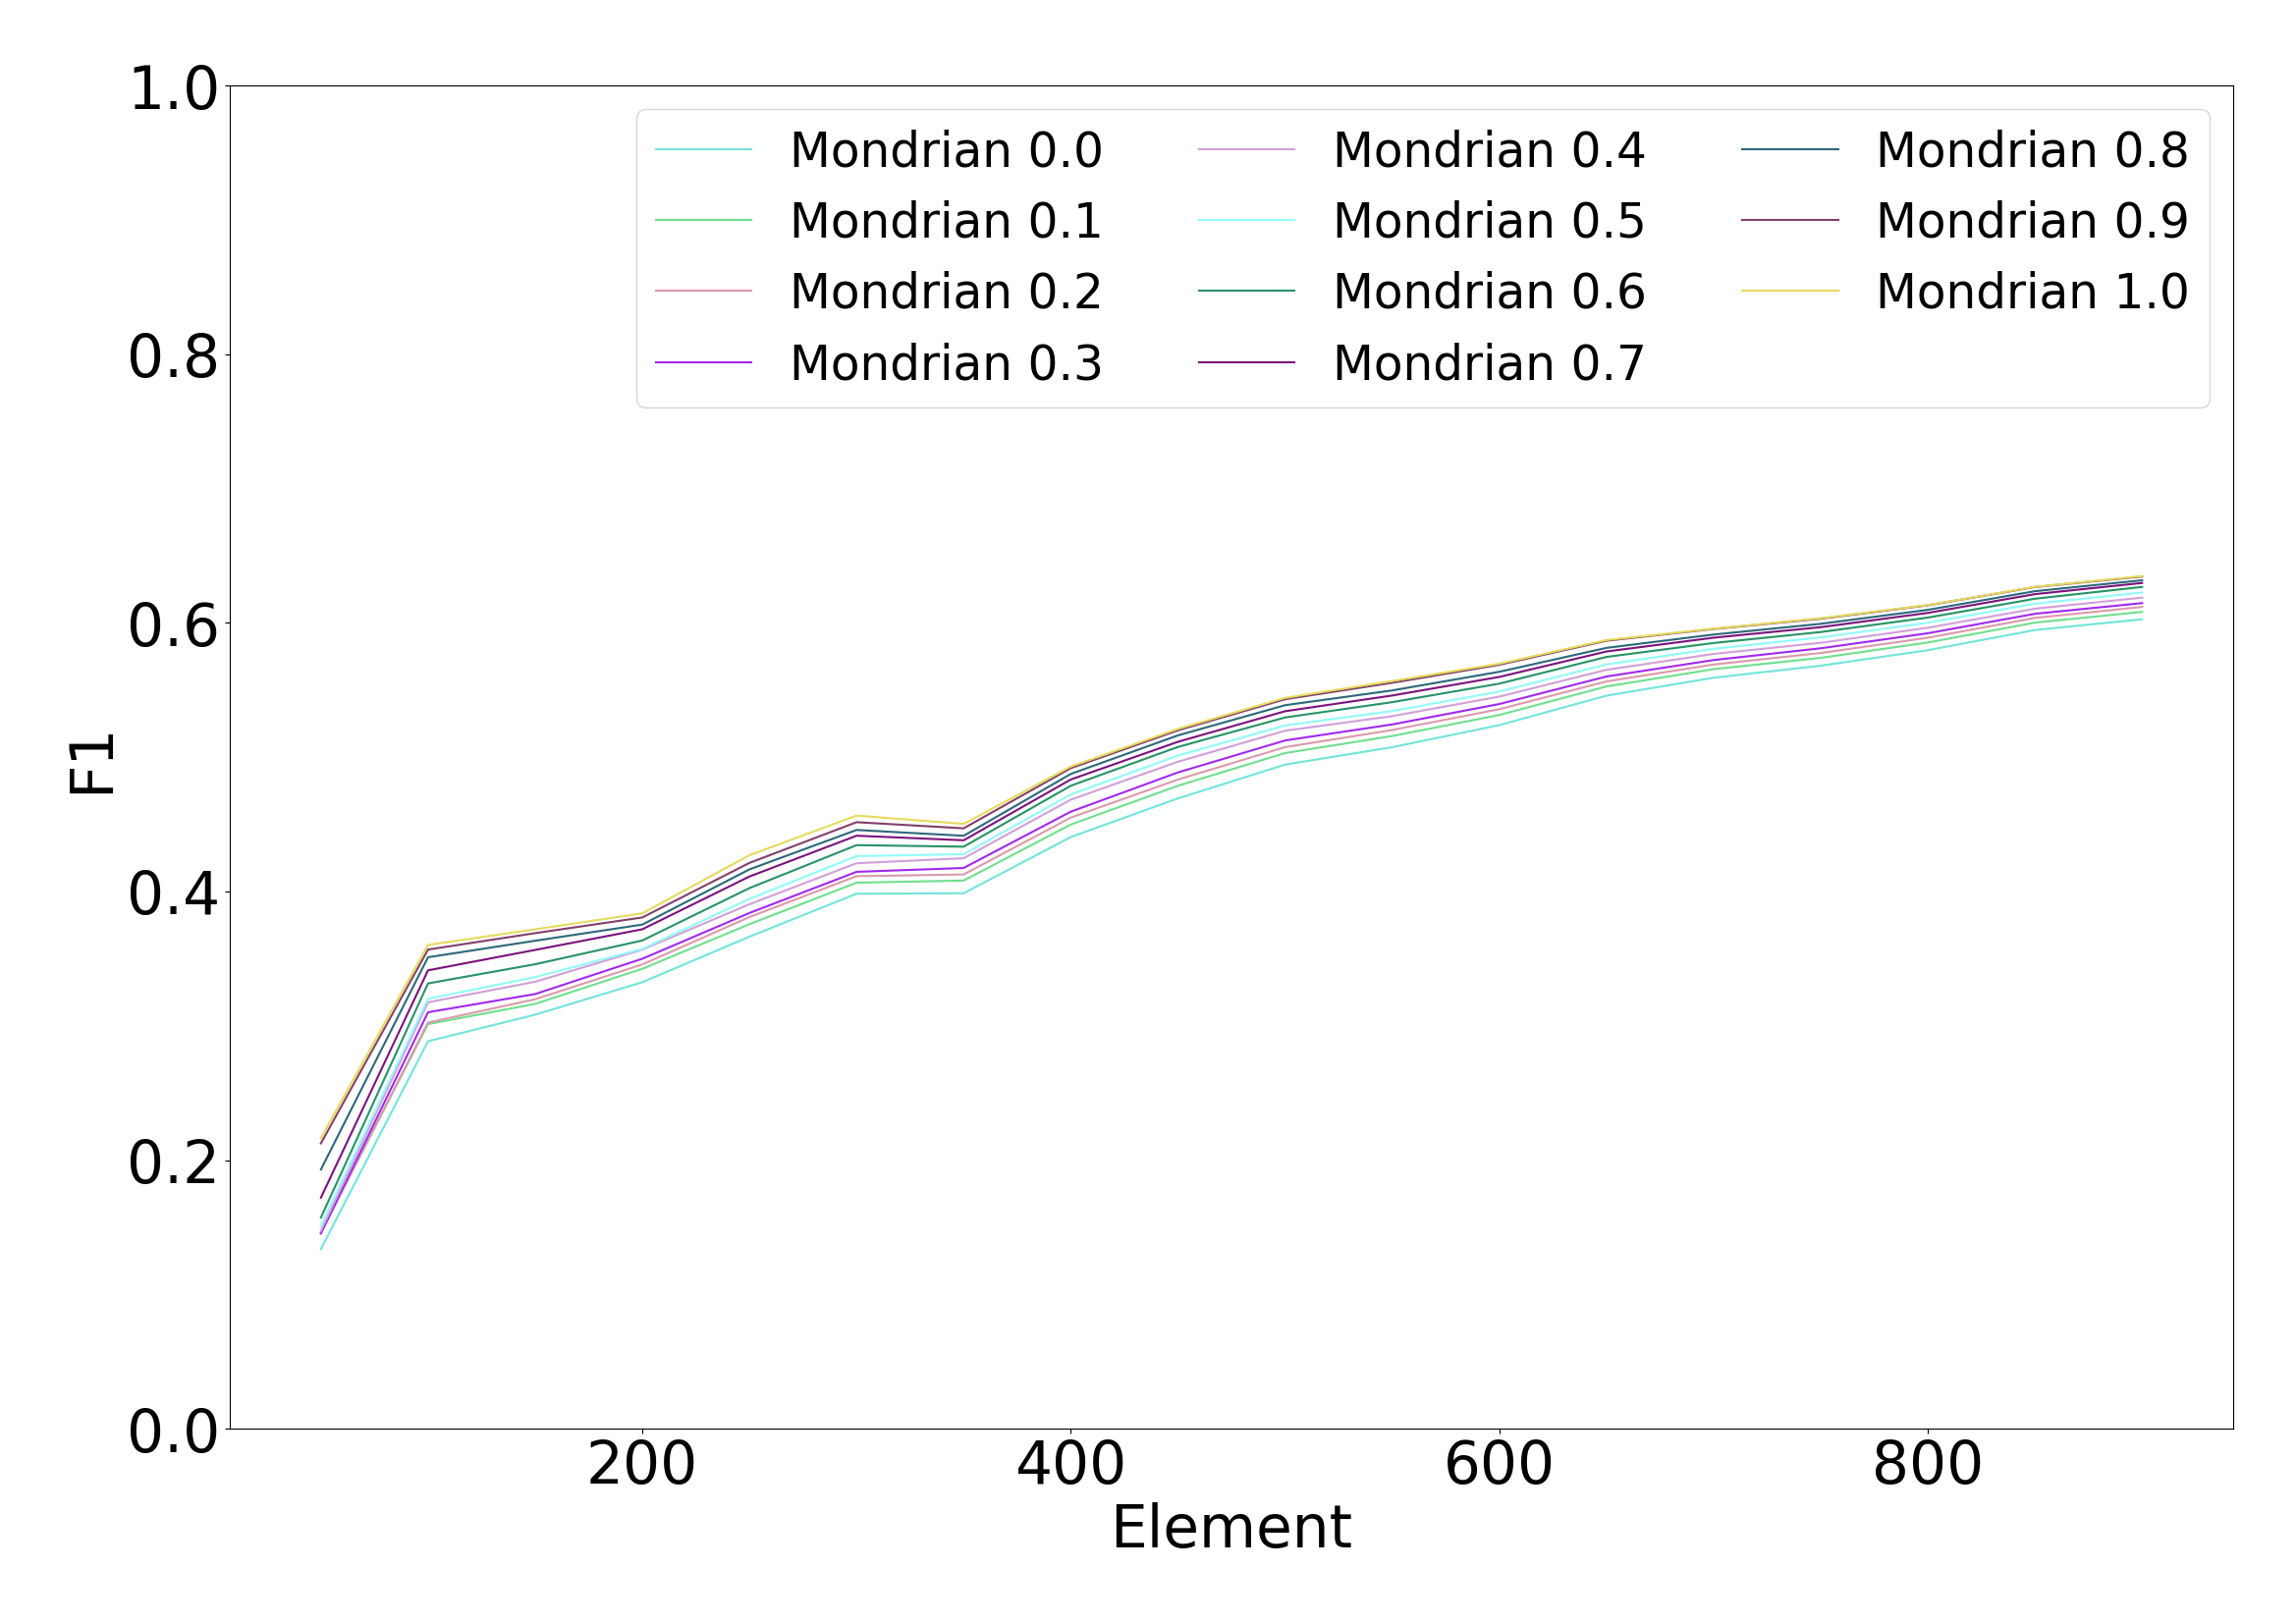
\includegraphics[width=\textwidth]{figures/calibration_mondrian_discount.png}
		 \caption{Impact of the discount factor with 10 trees, a budget of $1.0$, and a base count of $0.1$.}
		 \label{fig:mondrian-discount}
	 \end{subfigure}
		\caption{Hyperparameters tuning for Mondrian with first subject of \banosdataset dataset.}
		\label{fig:mondrian-tuning}
\end{figure}


% vim: tw=80 ts=2
